\documentclass[a4paper,12pt]{book}
\usepackage{amsmath,amsfonts,amssymb,amsthm,graphicx,hyperref,booktabs}
\usepackage[mathscr]{eucal}
\usepackage[a4paper,inner=1.5cm,outer=3cm,top=2cm,bottom=3cm,bindingoffset=1cm]{geometry}
\usepackage[numbers,sort&compress]{natbib}

\usepackage{listings} 
\lstset{                 
basicstyle=\ttfamily,   % code in typewriter font
numbers=left,           % where to put the line-numbers
numberstyle=\tiny,      % the size of the fonts used for the line-numbers
numbersep=5pt,          % how far the line-numbers are from the code
frame=single,           % adds a frame around the code
breaklines=true,        % sets automatic line breaking
columns=flexible        % important!
}

% 中文配置
\usepackage{xeCJK}
\setCJKmainfont{cwTeX Q Ming Medium}
\defaultCJKfontfeatures{AutoFakeBold=4,AutoFakeSlant=.4} 
\newCJKfontfamily\Kai{cwTeX Q Kai Medium} 
\newCJKfontfamily\Hei{cwTeX Q Hei Bold}
\newCJKfontfamily\Yuan{cwTeX Q Yuan Medium}
\newCJKfontfamily\Ming{cwTeX Q Ming Medium}
\newCJKfontfamily\Song{cwTeX Q Fangsong Medium}

\theoremstyle{definition}
\newtheorem{lmm}{Lemma}
\newtheorem{thm}{Theorem}
\newtheorem{dfn}{Definition}
\newtheorem{cor}{Corollary}
\newtheorem{prp}{Proposition}
\newtheorem{ex}{Example}
\newtheorem{prob}{Problem}

% Definition of various shortcuts.
\DeclareMathOperator\curl{curl}
\DeclareMathOperator\divv{div}
%\DeclareMathOperator\curl{\nabla\times}
%\DeclareMathOperator\divv{\nabla\cdot}
\DeclareMathOperator\Curlv{{\bf curl}_\Gamma}
\DeclareMathOperator\im{\Im}
\DeclareMathOperator\re{\Re}
\DeclareMathOperator\comp{\sf{K}}
\DeclareMathOperator\img{\EuScript{R}}
\DeclareMathOperator\pv{pv}
\DeclareMathOperator\dom{dom}
\DeclareMathOperator\nul{\EuScript{N}}
\DeclareMathOperator\rank{rk}
\DeclareMathOperator\col{col}
\DeclareMathOperator\range{range}
\DeclareMathOperator\dist{dist}
\newcommand\bdr{\Gamma}
\newcommand\Div{\divv_\Gamma}
\newcommand\Curl{\curl_\Gamma}
\newcommand\lTS{{\bf L}^2_\text{t}(\mathbb{S}^2)}
\newcommand\lTD{{\bf H}^{-\frac{1}{2}}(\Div)}
\newcommand\lTC{{\bf H}^{-\frac{1}{2}}(\Curl)}
\newcommand\lT{L_{2,\text{t}}(\bdr)}
\newcommand\nltwo[1]{\|#1\|_{L_2(\bdr)}}
\newcommand\nltwod[1]{\|#1\|_{\lTD}}
\newcommand\nltwoc[1]{\|#1\|_{\lTC}}
\newcommand\intv[1]{\int_{\Omega}#1\,\text{d}V}
\newcommand\ints[1]{\int_{\bdr}#1\,\text{d}\sigma}
\newcommand\intvv[1]{\int_{\Omega}#1}
\newcommand\intss[1]{\int_{\bdr}#1}
\newcommand\prb[1]{\begin{prob}#1\end{prob}}
\newcommand\sol[1]{\begin{proof}[Solution]#1\end{proof}}
  
% Trick for defining 'phantom' 
\newcommand\relphantom[1]{\mathrel{\phantom{#1}}}

% number within chapter: e.g.(1.1)
\numberwithin{equation}{chapter}
\numberwithin{thm}{chapter}
\numberwithin{prp}{chapter}
\numberwithin{lmm}{chapter}
\numberwithin{dfn}{chapter}
\numberwithin{cor}{chapter}

% principal value integral
\def\Xint#1{\mathchoice
  {\XXint\displaystyle\textstyle{#1}} 
  {\XXint\textstyle\scriptstyle{#1}} 
  {\XXint\scriptstyle\scriptscriptstyle{#1}} 
  {\XXint\scriptscriptstyle\scriptscriptstyle{#1}} 
\!\int}

\def\XXint#1#2#3{{\setbox0=\hbox{$#1{#2#3}{\int}$ }
\vcenter{\hbox{$#2#3$ }}\kern-.56\wd0}}
\def\ddashint{\Xint=}
\def\dashint{\Xint-}

% in tables with \toprule, set 12pt vertical space
\setlength{\abovetopsep}{12pt}

\begin{document}

\author{Chang-ye Tu}
\title{Electromagnetic Scattering Problems in Chiral Media}
\date{\today}
\maketitle
\tableofcontents

\chapter{Introduction}

\section{Preamble}

In this work, we study the scattering problem of time-harmonic electromagnetic waves by a bounded obstacle embedded in another medium. 

\section{Electromagnetic Field Equations}

In the absence of electrical charges and currents, the macroscopic time-dependent Maxwell equations of electromagnetism are
\begin{equation}\label{eq:maxorig}
  \begin{split}
  &\divv\mathcal{D} = 0 \\ 
  &\divv\mathcal{B} = 0 \\
  &\curl\mathcal{E}+\frac{\partial\mathcal{B}}{\partial t} = 0 \\
  &\curl\mathcal{H}-\frac{\partial\mathcal{D}}{\partial t} = 0 
  \end{split}
\end{equation}
where $\mathcal{D}$ denotes the electric displacement, $\mathcal{B}$ the magnetic induction, $\mathcal{E}$ the electric field, and $\mathcal{H}$ the magnetic field. By ``time-harmonic'' the fields are of the form 
\begin{align*}
  \mathcal{D}(x, t) &= \re\{D(x)e^{-i\omega t}\}\\
  \mathcal{B}(x, t) &= \re\{B(x)e^{-i\omega t}\}\\ 
  \mathcal{E}(x, t) &= \re\{E(x)e^{-i\omega t}\}\\
  \mathcal{H}(x, t) &= \re\{H(x)e^{-i\omega t}\}\\ 
\end{align*}
where $x\in\mathbb{R}^3$ and $\omega$ denotes the frequency. Under the time-harmonic assumption, the Maxwell equations \eqref{eq:maxorig} become 
\begin{equation}\label{eq:maxhrm}
  \begin{split}
  &\divv D = 0\\ 
  &\divv B = 0\\
  &\curl E - i\omega B = 0\\
  &\curl H + i\omega D = 0 
  \end{split}
\end{equation}

In order to proceed, the constitutive relations between $D, E$ and $B, H$, which specify the response of bound charge and current to the applied fields, should be introduced. 

For chiral media which obey the Drude-Born-Fedorov constitutive relations
\begin{equation}
\begin{split}\label{eq:born}
  D &= \varepsilon(E + \beta\curl E), \\
  B &= \mu(H + \beta\curl H),
\end{split}
\end{equation}
where $\varepsilon$ denotes the electric permittivity, $\mu$ the magnetic permittivity and $\beta$ the chirality measure, the Maxwell equations \eqref{eq:maxhrm} become
\begin{equation}\label{eq:maxcnoh}
\begin{split}
  &\divv E = 0 \\
  &\divv H = 0 \\
  &\curl E - i\omega\mu(H+\beta\curl H) = 0\\
  &\curl H + i\omega\varepsilon(E+\beta\curl E) = 0
\end{split}
\end{equation}

In this work
\begin{figure}
\centering
  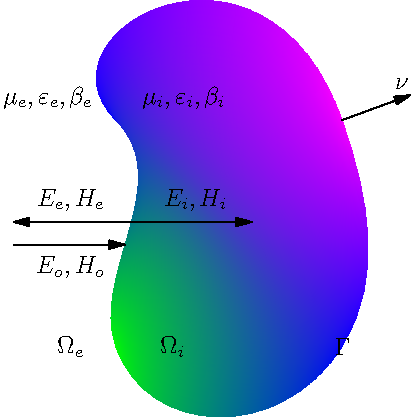
\includegraphics{fig1.pdf}
  \caption{Problem Settings}  
\label{fig:1}
\end{figure}

\begin{equation}
\begin{split}
  \nu\times\left(E_\text{e} + E_\text{o}\right) &= \nu\times E_\text{i} \\
  \nu\times\left(H_\text{e} + H_\text{o}\right) &= \nu\times H_\text{i} \\
\end{split}
\end{equation}

\subsection{Homogeneous Media}

For homogeneous media with constant $\mu,\varepsilon$ independent of location, we substitute
\begin{equation}\label{eq:scale}
  \begin{split}
    E &:= \sqrt{\mu}E \\
    H &:= \sqrt{\varepsilon}H 
  \end{split}
\end{equation} 
into \eqref{eq:maxcnoh} to get
\begin{equation}\label{eq:maxch}
\begin{split}
  &\divv E = 0 \\
  &\divv H = 0 \\
  &\curl E - ik(H+\beta\curl H) = 0\\
  &\curl H + ik(E+\beta\curl E) = 0
\end{split}
\end{equation}
where
$$k=\omega\sqrt{\mu\varepsilon}.$$ 

It is convenient to introduce the auxilliary notation $U, U'$ as follows:
\begin{equation}
  \begin{split}
    &\text{if  }U=E\text{,  then  }U'=iH \\
    &\text{if  }U=H\text{,  then  }U'=-iE \\
  \end{split}
\end{equation}
Here $E, H$ are the solutions of \eqref{eq:maxch}. Note that 
\begin{align*}
  (U')'=U.
\end{align*}
With the $U$ notation we can summarize the last two equations of \eqref{eq:maxch} as
\begin{align}\label{eq:u00}
  \curl U = k U' + k\beta\curl U'.
\end{align}
From $(U')'=U$, we have
\begin{equation}\label{eq:u01}
  \begin{split}
    \curl U' &= k (U')' + k\beta\curl (U')' \\ 
             &= k U + k\beta\curl U.
  \end{split}
\end{equation}
Eliminate $\curl U'$ from \eqref{eq:u00}, \eqref{eq:u01}, we have 
\begin{align}\label{eq:gu}
  \curl U = \gamma^2\beta U + \frac{\gamma^2}{k} U'
\end{align}
where
\begin{align}
  \gamma^2 &=\frac{k^2}{1-k^2\beta^2} 
\end{align}
By taking the curl of \eqref{eq:gu} and using \eqref{eq:u01}, we have
\begin{align}
  \curl\curl U - 2\gamma^2\beta\curl U - \gamma^2 U = 0
\end{align}

With the scaling \eqref{eq:scale} performed in each region, the transmission boundary condition becomes
\begin{equation}
\begin{split}
  \nu\times\left(E_\text{e} + E_\text{o}\right) &= \delta\,\nu\times E_\text{i} \\
  \nu\times\left(H_\text{e} + H_\text{o}\right) &= \rho\,\nu\times H_\text{i} \\
\end{split}
\end{equation}
where
\begin{align}
  \delta = \sqrt{\frac{\mu_\text{i}}{\mu_\text{e}}}, \quad \rho= \sqrt{\frac{\varepsilon_\text{i}}{\varepsilon_\text{e}}}. 
\end{align}

\subsubsection{Bohren's Transformation}
By expanding \eqref{eq:gu}, we have
\begin{align}\label{eq:maxe}
  \left(1-k^2\beta^2\right)\curl E = ikH + k^2\beta E
\end{align}
and
\begin{align}\label{eq:maxh}
  \left(1-k^2\beta^2\right)\curl H = -ikE + k^2\beta H
\end{align}
The above two equations can be rewritten into matrix form:
\begin{align*}
 \begin{pmatrix}\curl E \\ \curl H\end{pmatrix} = \frac{1}{1-k^2\beta^2}\begin{pmatrix}k^2\beta & ik \\-ik & k^2\beta\end{pmatrix}\begin{pmatrix}E \\ H\end{pmatrix} := A\begin{pmatrix}E \\ H\end{pmatrix}\end{align*}
Computing the roots of the equation
\begin{align*}
  \det(A-\lambda I) &= \begin{vmatrix}
    \frac{k^2\beta}{1-k^2\beta^2} - \lambda & \frac{ik}{1-k^2\beta^2} \\
    \frac{-ik}{1-k^2\beta^2} & \frac{k^2\beta}{1-k^2\beta^2} - \lambda
  \end{vmatrix} \\
  &= \left(\lambda-\frac{k^2\beta}{1-k^2\beta^2}\right)^2 - \frac{k^2}{(1-k^2\beta^2)^2}\\
  &= \left(\lambda-\frac{k^2\beta}{1-k^2\beta^2}\right)^2 - \left(\frac{k}{1-k^2\beta^2}\right)^2 \\
  &= \left(\lambda-\frac{k^2\beta + k}{1-k^2\beta^2}\right)\left(\lambda-\frac{k^2\beta - k}{1-k^2\beta^2}\right) \\
  &= \left(\lambda-\frac{k(k\beta + 1)}{(1+k\beta)(1-k\beta)}\right)\left(\lambda-\frac{k(k\beta-1)}{(1+k\beta)(1-k\beta)}\right) \\
  &=\left(\lambda-\frac{k}{1-k\beta}\right)\left(\lambda + \frac{k}{1+k\beta}\right)\\
  &=0,
\end{align*}
the eigenvalues of $A$ are $\frac{k}{1 - k\beta}$ and $-\frac{k}{1 + k\beta}$ with corresponding orthonormal eigenvectors $\frac{1}{\sqrt{2}}(1, -i)^\top$ and $\frac{1}{\sqrt{2}}(1, i)^\top$. Let $P$ be the matrix formed by the eigenvectors as columns,
\begin{align*}
  P = \frac{1}{\sqrt{2}}\begin{pmatrix}1 & 1 \\ -i & i\end{pmatrix}
\end{align*}
then 
\begin{align*}
  P^{-1} = \frac{1}{\sqrt{2}}\begin{pmatrix}1 & i \\ 1 & -i\end{pmatrix}
\end{align*}
is the basis transformation matrix. Hence if we set
\begin{equation}\label{eq:bohren}
\begin{split}
  Q_\text{l} &= E + iH \\
  Q_\text{r} &= E - iH
\end{split}
\end{equation}
the Maxwell equations \eqref{eq:maxe}, \eqref{eq:maxh} are transformed into the diagonalized form
\begin{align}\label{eq:qlr} 
  \curl Q_\text{l} &= \gamma_\text{l}\,Q_\text{l}\\
  \curl Q_\text{r} &= -\gamma_\text{r}\,Q_\text{r}
\end{align}
where
\begin{equation}
\begin{split}\label{eq:glr}
  \gamma_\text{l} &= \frac{k}{1 - k\beta},\\
  \gamma_\text{r} &= \frac{k}{1 + k\beta}
\end{split}
\end{equation}
and this can be directly verified. From \eqref{eq:bohren}, we have 
\begin{equation}\label{eq:bohren1}
\begin{split}
  E &= \frac{1}{2}\left(Q_\text{r} + Q_\text{l}\right) \\
  H &= \frac{i}{2}\left(Q_\text{r} - Q_\text{l}\right)
\end{split}
\end{equation}
Substituting \eqref{eq:bohren1} into \eqref{eq:u01}, we have
\begin{align*}
  \curl\left(\frac{1}{2}\left(Q_\text{r} + Q_\text{l}\right)\right) - ik\left\{\frac{i}{2}\left(Q_\text{r} - Q_\text{l}\right)+\beta\curl\left(\frac{i}{2}\left(Q_\text{r} - Q_\text{l}\right)\right)\right\} &= 0 \\
  \curl\left(\frac{i}{2}\left(Q_\text{r} - Q_\text{l}\right)\right) + ik\left\{\frac{1}{2}\left(Q_\text{r} + Q_\text{l}\right)+\beta\curl\left(\frac{1}{2}\left(Q_\text{r} + Q_\text{l}\right)\right)\right\} &= 0
\end{align*}
which can be simplified as
\begin{align}
  \curl\left(Q_\text{r} + Q_\text{l}\right) + k\left(Q_\text{r} - Q_\text{l}\right) + k\beta\curl\left(Q_\text{r} - Q_\text{l}\right) &= 0 \label{eq:q00} \\
  \curl\left(Q_\text{r} - Q_\text{l}\right) + k\left(Q_\text{r} + Q_\text{l}\right) + k\beta\curl\left(Q_\text{r} + Q_\text{l}\right) &= 0 \label{eq:q01}
\end{align}
By performing \eqref{eq:q00}$+$\eqref{eq:q01}, \eqref{eq:q00}$-$\eqref{eq:q01} we recover \eqref{eq:qlr}.

Hereafter each of \eqref{eq:bohren}, \eqref{eq:bohren1} denotes ``Bohren's Transformation''.

%We say that the tuple $(E,H,k)$ solves Maxwell equations if
%\begin{align*}
%  &\divv E = 0\\
%  &\divv H = 0\\
%  &\curl E - ikH = 0\\
%  &\curl H + ikE = 0\\
%\end{align*}
%
%It is clear that $(Q_\text{l}, -iQ_\text{l}, \gamma_\text{l})$ and $(Q_\text{r}, iQ_\text{r}, \gamma_\text{r})$ solve Maxwell equations and this fact allows us to reuse the representation theorem established in achiral cases.
%
%\begin{align*}
%  -2U &= C\{\nu\times U\} + \frac{1}{k} F\{\nu\times U'\}
%\end{align*}

\subsubsection{Reduction to Two Dimension}

Starting from
\begin{align}
  \left(1-k^2\beta^2\right)\curl E &= ikH + k^2\beta E \label{eq:ex00}\\
  \left(1-k^2\beta^2\right)\curl H &= -ikE + k^2\beta H\label{eq:ex01}
\end{align}
Note that all $\partial_3$ derivatives vanish, thus the expression of $\curl$ becomes
\begin{align*}
  \curl U = \begin{pmatrix}
    \partial_2 U_3-\partial_3 U_2 \\
    \partial_3 U_1-\partial_1 U_3 \\
    \partial_1 U_2-\partial_2 U_1 \\
  \end{pmatrix} 
  = \begin{pmatrix}
    \partial_2 U_3 \\
    -\partial_1 U_3 \\
    \partial_1 U_2-\partial_2 U_1 \\
  \end{pmatrix} 
\end{align*}
Expanding \eqref{eq:ex00}, we have
\begin{align*}
  \left(1-k^2\beta^2\right)\begin{pmatrix}\partial_2 E_3\\ -\partial_1 E_3 \\ \partial_1 E_2 -\partial_2 E_1\end{pmatrix} = ik\begin{pmatrix}H_1\\H_2\\H_3\end{pmatrix} + k^2\beta\begin{pmatrix}E_1\\E_2\\E_3\end{pmatrix}
\end{align*}
The first row reads
\begin{align*}
  \left(1-k^2\beta^2\right)\partial_2 E_3 = ik H_1 + k^2\beta E_1
\end{align*}
Differentiate with $x_2$,
\begin{align}\label{eq:he00}
  \left(1-k^2\beta^2\right)\partial_2^2 E_3 = ik \,\partial_2 H_1 + k^2\beta\,\partial_2 E_1
\end{align}
The second row reads
\begin{align*}
  -\left(1-k^2\beta^2\right)\partial_1 E_3 = ik H_2 + k^2\beta E_2
\end{align*}
Differentiate with $x_1$,
\begin{align}\label{eq:he01}
  -\left(1-k^2\beta^2\right)\partial_1^2 E_3 = ik \,\partial_1 H_2 + k^2\beta\,\partial_1 E_2
\end{align}
Combining \eqref{eq:he00}, \eqref{eq:he01}, we obtain the equation
\begin{equation}
\begin{split}
  &\left(1-k^2\beta^2\right)\left(\partial_1^2 + \partial_2^2\right)E_3 \\
  &= ik\left(\partial_2 H_1 - \partial_1 H_2\right) + k^2\beta\left(\partial_2 E_1 - \partial_1 E_2\right) \\
  &= \frac{1}{1-k^2\beta^2}\left\{ik\left(ik E_3 - k^2\beta H_3\right) - k^2\beta\left(ik H_3 + k^2\beta E_3\right)\right\} \\
  &= \frac{1}{1-k^2\beta^2}\left\{-\left(k^2 + k^4\beta^2\right)E_3 - 2 i k^3\beta H_3\right\} \\
\end{split}
\end{equation}
Similarly, by expanding \eqref{eq:ex01}, we have
\begin{align*}
  \left(1-k^2\beta^2\right)\begin{pmatrix}\partial_2 H_3\\ -\partial_1 H_3 \\ \partial_1 H_2 -\partial_2 H_1\end{pmatrix} = -ik\begin{pmatrix}E_1\\E_2\\E_3\end{pmatrix} + k^2\beta\begin{pmatrix}H_1\\H_2\\H_3\end{pmatrix}
\end{align*}
The first row reads
\begin{align*}
  \left(1-k^2\beta^2\right)\partial_2 H_3 = -ik E_1 + k^2\beta H_1
\end{align*}
Differentiate with $x_2$, 
\begin{align}\label{eq:hh00}
  \left(1-k^2\beta^2\right)\partial_2^2 H_3 = -ik \,\partial_2 E_1 + k^2\beta\,\partial_2 H_1
\end{align}
The second row reads
\begin{align*}
  -\left(1-k^2\beta^2\right)\partial_1 H_3 = -ik E_2 + k^2\beta H_2
\end{align*}
Differentiate with $x_1$,
\begin{align}\label{eq:hh01}
  -\left(1-k^2\beta^2\right)\partial_1^2 H_3 = -ik \,\partial_1 E_2 + k^2\beta\,\partial_1 H_2
\end{align}
Combining \eqref{eq:hh00}, \eqref{eq:hh01}, we obtain the equation
\begin{equation}
\begin{split}
  &\left(1-k^2\beta^2\right)\left(\partial_1^2 + \partial_2^2\right)H_3 \\
  &=-ik\left(\partial_2 E_1 - \partial_1 E_2\right) + k^2\beta\left(\partial_2 H_1 - \partial_1 H_2\right)\\
  &= \frac{1}{1-k^2\beta^2}\left\{ik\left(ik H_3 + k^2\beta E_3\right) + k^2\beta\left(ik E_3 - k^2\beta H_3\right)\right\} \\
  &= \frac{1}{1-k^2\beta^2}\left\{-\left(k^2 + k^4\beta^2\right)H_3 + 2 i k^3\beta E_3\right\} \\
\end{split}
\end{equation}

Now we derive the relations between $E_1, H_1, E_2, H_2$ and $E_3, H_3$. Starting from the first two rows of \eqref{eq:ex00}, \eqref{eq:ex01},  
\begin{align*}
  \left(1-k^2\beta^2\right)\partial_2 E_3 &= ik H_1 + k^2\beta E_1 \\
  -\left(1-k^2\beta^2\right)\partial_1 E_3 &= ik H_2 + k^2\beta E_2 \\
  \left(1-k^2\beta^2\right)\partial_2 H_3 &= -ik E_1 + k^2\beta H_1 \\
  -\left(1-k^2\beta^2\right)\partial_1 H_3 &= -ik E_2 + k^2\beta H_2 \\
\end{align*}
Rewriting in matrix form:
\begin{align*}
  \begin{pmatrix}
    k^2\beta & 0 & ik & 0 \\
    0 & k^2\beta & 0 & ik \\
    -ik & 0 & k^2\beta & 0 \\
    0 & -ik & 0 & k^2\beta \\
  \end{pmatrix} 
  \begin{pmatrix}
    E_1 \\ E_2 \\ H_1 \\ H_2
  \end{pmatrix} =
  \left(1-k^2\beta^2\right)
  \begin{pmatrix}
    \partial_2 E_3 \\ -\partial_1 E_3 \\ \partial_2 H_3 \\ -\partial_1 H_3 \\ 
  \end{pmatrix}
\end{align*}
The inverse matrix of the left hand side is
\begin{align*}
  \begin{pmatrix}
    k^2\beta & 0 & ik & 0 \\
    0 & k^2\beta & 0 & ik \\
    -ik & 0 & k^2\beta & 0 \\
    0 & -ik & 0 & k^2\beta \\
  \end{pmatrix}^{-1} = \frac{1}{1-k^2\beta^2}
  \begin{pmatrix}
    -\beta & 0 & \frac{i}{k} & 0 \\
    0 & -\beta & 0 & \frac{i}{k} \\
    -\frac{i}{k} & 0 & -\beta & 0 \\
    0 & -\frac{i}{k} & 0 & -\beta \\
  \end{pmatrix} 
\end{align*}
Hence
\begin{align*}
  \begin{pmatrix}
    E_1 \\ E_2 \\ H_1 \\ H_2
  \end{pmatrix} 
  &= 
  \begin{pmatrix}
    -\beta & 0 & \frac{i}{k} & 0 \\
    0 & -\beta & 0 & \frac{i}{k} \\
    -\frac{i}{k} & 0 & -\beta & 0 \\
    0 & -\frac{i}{k} & 0 & -\beta \\
  \end{pmatrix}
  \begin{pmatrix}
    \partial_2 E_3 \\ -\partial_1 E_3 \\ \partial_2 H_3 \\ -\partial_1 H_3 \\ 
  \end{pmatrix}
  \\ 
  &=
  \begin{pmatrix}
    -\beta\partial_2 E_3 + \frac{i}{k}\partial_2 H_3 \\
    \beta\partial_1 E_3  - \frac{i}{k}\partial_1 H_3 \\
    -\beta\partial_2 H_3  - \frac{i}{k}\partial_2 E_3 \\
    \beta\partial_1 H_3  + \frac{i}{k}\partial_1 E_3 \\
  \end{pmatrix}
\end{align*}
We have
\begin{equation}\label{eq:eh2}
  \begin{split}
    E_1&=-\beta\partial_2 E_3 + \frac{i}{k}\partial_2 H_3 \\
    E_2&=\beta\partial_1 E_3  - \frac{i}{k}\partial_1 H_3 \\
    H_1&=-\beta\partial_2 H_3  - \frac{i}{k}\partial_2 E_3 \\
    H_2&=\beta\partial_1 H_3  + \frac{i}{k}\partial_1 E_3
  \end{split}
\end{equation}

Now we derive terms used in formulating boundary conditions. In two dimensional case, the third component of $\nu$ vanishes. For any field $U$ we have 
\begin{equation}
\begin{split}
  \nu\times U = \begin{pmatrix}\nu_1 \\ \nu_2 \\ 0\end{pmatrix} 
    \times 
    \begin{pmatrix}U_1\\U_2\\U_3\end{pmatrix} =
      \begin{pmatrix}\nu_2\,U_3\\-\nu_1\,U_3\\ \nu_1\,U_2-\nu_2\,U_1\end{pmatrix}
\end{split}
\end{equation}
The term that would need further deduction is $\nu_1\,U_2-\nu_2\,U_1$. Combining \eqref{eq:eh2}, we have
\begin{equation}\label{eq:nuE}
\begin{split}
  \nu_1 E_2 - \nu_2 E_1 &= \nu_1\left(\beta\partial_1 E_3 - \frac{i}{k}\partial_1 H_3\right) - \nu_2\left(-\beta\partial_2 E_3 + \frac{i}{k}\partial_2 H_3\right) \\
  &= \beta\nu\cdot\nabla E_3 - \frac{i}{k}\nu\cdot\nabla H_3\\
  &= \beta\frac{\partial E_3}{\partial\nu} - \frac{i}{k}\frac{\partial H_3}{\partial\nu}
\end{split}
\end{equation}
and
\begin{equation}\label{eq:nuH}
\begin{split}
  \nu_1 H_2 - \nu_2 H_1 &= \nu_1\left(\beta\partial_1 H_3 + \frac{i}{k}\partial_1 E_3\right) - \nu_2\left(-\beta\partial_2 H_3 - \frac{i}{k}\partial_2 E_3\right) \\
  &= \beta\nu\cdot\nabla H_3 + \frac{i}{k}\nu\cdot\nabla E_3\\
  &= \beta\frac{\partial H_3}{\partial\nu} + \frac{i}{k}\frac{\partial E_3}{\partial\nu}
\end{split}
\end{equation}
The boundary conditions are
\begin{align}
  \nu\times E_\text{o} &= \delta\,\nu\times E_\text{i} - \nu\times E_\text{e}\label{eq:bc00}\\
  \nu\times H_\text{o} &= \rho\,\nu\times H_\text{i} - \nu\times H_\text{e}\label{eq:bc01}
\end{align}
Expanding the first two rows of \eqref{eq:bc00}, we have
\begin{align*}
  \nu_2 E_{\text{o}3} &= \delta\,\nu_2 E_{\text{i}3} -\nu_2 E_{\text{e}3} \\
  -\nu_1 E_{\text{o}3} &= -\delta\,\nu_1 E_{\text{i}3} + \nu_1 E_{\text{e}3} \\
\end{align*}
Here the term $E_{\text{o}3}$ denotes the third component of $E_{\text{o}}$; the meaning of similar terms $E_{\text{i}3}$, $E_{\text{e}3}$, $E_{\text{e}1}$, etc. should be clear. The two equations are in fact only one, namely
\begin{align}\label{eq:bc2d00}
  E_{\text{o}3} &= \delta\,E_{\text{i}3} - E_{\text{e}3}
\end{align}
Similarly, expanding the first two rows of \eqref{eq:bc01}, we have
\begin{align*}
  \nu_2 H_{\text{o}3} &= \rho\,\nu_2 H_{\text{i}3} -\nu_2 H_{\text{e}3} \\
  -\nu_1 H_{\text{o}3} &= -\rho\,\nu_1 H_{\text{i}3} + \nu_1 H_{\text{e}3} \\
\end{align*}
which can be summarized as 
\begin{align}\label{eq:bc2d01}
  H_{\text{o}3} &= \rho\,H_{\text{i}3} - H_{\text{e}3} 
\end{align}
With the expressions \eqref{eq:nuE}, \eqref{eq:nuH}, the remaining two boundary conditions are
\begin{align}\label{eq:bc2d02}
  \nu_1 E_{\text{o}2} - \nu_2 E_{\text{o}1} &= \delta\left(\beta_\text{i}\frac{\partial E_{\text{i}3}}{\partial\nu} - \frac{i}{k_\text{i}}\frac{\partial H_{\text{i}3}}{\partial\nu}\right) -\left(\beta_\text{e}\frac{\partial E_{\text{e}3}}{\partial\nu} - \frac{i}{k_\text{e}}\frac{\partial H_{\text{e}3}}{\partial\nu}\right)
\end{align}
and 
\begin{align}\label{eq:bc2d03}
  \nu_1 H_{\text{o}2} - \nu_2 H_{\text{o}1} &= \rho\left(\beta_\text{i}\frac{\partial H_{\text{i}3}}{\partial\nu} + \frac{i}{k_\text{i}}\frac{\partial E_{\text{i}3}}{\partial\nu}\right) -\left(\beta_\text{e}\frac{\partial H_{\text{e}3}}{\partial\nu} + \frac{i}{k_\text{e}}\frac{\partial E_{\text{e}3}}{\partial\nu}\right) 
\end{align}
Recall the Bohren's transformation in outer environment and inner obstacle:
\begin{equation}\label{eq:bohrenc}
\begin{split}
  E_{\text{e}3} &= \frac{1}{2}\left(Q_\text{er} + Q_\text{el}\right) \\
  H_{\text{e}3} &= \frac{i}{2}\left(Q_\text{er} - Q_\text{el}\right) \\
  E_{\text{i}3} &= \frac{1}{2}\left(Q_\text{ir} + Q_\text{il}\right) \\
  H_{\text{i}3} &= \frac{i}{2}\left(Q_\text{ir} - Q_\text{il}\right) \\
\end{split}
\end{equation}
Apply \eqref{eq:bohrenc} in \eqref{eq:bc2d00},
\begin{align*}
  E_{\text{o}3} &= \frac{\delta}{2}(Q_\text{ir} + Q_\text{il}) - \frac{1}{2}(Q_\text{er} + Q_\text{el}) \\
\end{align*}
Apply \eqref{eq:bohrenc} in \eqref{eq:bc2d01},
\begin{align*}
  H_{\text{o}3} &= \frac{i\rho}{2}(Q_\text{ir} - Q_\text{il}) -\frac{i}{2}(Q_\text{er} - Q_\text{el}) \\
\end{align*}
Apply \eqref{eq:bohrenc} in \eqref{eq:bc2d02},
\begin{align*}
  -\nu_1 E_{\text{o}2} + \nu_2 E_{\text{o}1} &= \delta\,\left\{\beta_\text{i}\frac{\partial}{\partial\nu}\left(\frac{1}{2}(Q_\text{ir} + Q_\text{il})\right) - \frac{i}{k_\text{i}}\frac{\partial}{\partial\nu}\left(\frac{i}{2}\left(Q_\text{ir} - Q_\text{il}\right)\right)\right\} \\
  &-\left\{\beta_\text{e}\frac{\partial}{\partial\nu}\left(\frac{1}{2}(Q_\text{er} + Q_\text{el})\right) - \frac{i}{k_\text{e}}\frac{\partial}{\partial\nu}\left(\frac{i}{2}\left(Q_\text{er} - Q_\text{el}\right)\right)\right\} \\
  &=\frac{\delta}{2}\left(\frac{1 + k_\text{i}\beta_\text{i}}{k_\text{i}}\frac{\partial Q_\text{ir}}{\partial\nu} - \frac{1 - k_\text{i}\beta_\text{i}}{k_\text{i}}\frac{\partial Q_\text{il}}{\partial\nu}\right) \\
  &-\frac{1}{2}\left(\frac{1 + k_\text{e}\beta_\text{e}}{k_\text{e}}\frac{\partial Q_\text{er}}{\partial\nu} - \frac{1 - k_\text{e}\beta_\text{e}}{k_\text{e}}\frac{\partial Q_\text{el}}{\partial\nu}\right) \\
  &=\frac{\delta}{2}\left(\frac{1}{\gamma_\text{ir}}\frac{\partial Q_\text{ir}}{\partial\nu} - \frac{1}{\gamma_\text{il}}\frac{\partial Q_\text{il}}{\partial\nu}\right) -\frac{1}{2}\left(\frac{1}{\gamma_\text{er}}\frac{\partial Q_\text{er}}{\partial\nu} - \frac{1}{\gamma_\text{el}}\frac{\partial Q_\text{el}}{\partial\nu}\right) \\
\end{align*}
Apply \eqref{eq:bohrenc} in \eqref{eq:bc2d03},
\begin{align*}
  -\nu_1 H_{\text{o}2} + \nu_2 H_{\text{o}1} &= \rho\,\left\{\beta_\text{i}\frac{\partial}{\partial\nu}\left(\frac{i}{2}(Q_\text{ir} - Q_\text{il})\right) + \frac{i}{k_\text{i}}\frac{\partial}{\partial\nu}\left(\frac{1}{2}\left(Q_\text{ir} + Q_\text{il}\right)\right)\right\} \\
  &-\left\{\beta_\text{e}\frac{\partial}{\partial\nu}\left(\frac{i}{2}(Q_\text{er} - Q_\text{el})\right) + \frac{i}{k_\text{e}}\frac{\partial}{\partial\nu}\left(\frac{1}{2}\left(Q_\text{er} + Q_\text{el}\right)\right)\right\} \\
  &=\frac{i\rho}{2}\left(\frac{1 + k_\text{i}\beta_\text{i}}{k_\text{i}}\frac{\partial Q_\text{ir}}{\partial\nu} + \frac{1 - k_\text{i}\beta_\text{i}}{k_\text{i}}\frac{\partial Q_\text{il}}{\partial\nu}\right) \\
  &-\frac{i}{2}\left(\frac{1 + k_\text{e}\beta_\text{e}}{k_\text{e}}\frac{\partial Q_\text{er}}{\partial\nu} + \frac{1 - k_\text{e}\beta_\text{e}}{k_\text{e}}\frac{\partial Q_\text{el}}{\partial\nu}\right) \\
  &=\frac{i\rho}{2}\left(\frac{1}{\gamma_\text{ir}}\frac{\partial Q_\text{ir}}{\partial\nu} + \frac{1}{\gamma_\text{il}}\frac{\partial Q_\text{il}}{\partial\nu}\right) -\frac{i}{2}\left(\frac{1}{\gamma_\text{er}}\frac{\partial Q_\text{er}}{\partial\nu} + \frac{1}{\gamma_\text{el}}\frac{\partial Q_\text{el}}{\partial\nu}\right)
\end{align*}
By writing
\begin{equation}
\begin{split}
  v_0 &:= E_{\text{o}3} \\
  w_0 &:= H_{\text{o}3} \\
  v_1 &:= -\nu_1 E_{\text{o}2} + \nu_2 E_{\text{o}1} \\
  w_1 &:= -\nu_1 H_{\text{o}2} + \nu_2 H_{\text{o}1} \\
\end{split}
\end{equation}
we collect the previous four equations as the ``master equations'':
\begin{equation}\label{eq:master}
\begin{split}
  v_0 &= \frac{\delta}{2}(Q_\text{ir} + Q_\text{il}) - \frac{1}{2}(Q_\text{er} + Q_\text{el}) \\
  w_0 &= \frac{i\rho}{2}(Q_\text{ir} - Q_\text{il}) -\frac{i}{2}(Q_\text{er} - Q_\text{el}) \\
  v_1 &=\frac{\delta}{2}\left(\frac{1}{\gamma_\text{ir}}\frac{\partial Q_\text{ir}}{\partial\nu} - \frac{1}{\gamma_\text{il}}\frac{\partial Q_\text{il}}{\partial\nu}\right) -\frac{1}{2}\left(\frac{1}{\gamma_\text{er}}\frac{\partial Q_\text{er}}{\partial\nu} - \frac{1}{\gamma_\text{el}}\frac{\partial Q_\text{el}}{\partial\nu}\right) \\
  w_1 &=\frac{i\rho}{2}\left(\frac{1}{\gamma_\text{ir}}\frac{\partial Q_\text{ir}}{\partial\nu} + \frac{1}{\gamma_\text{il}}\frac{\partial Q_\text{il}}{\partial\nu}\right) -\frac{i}{2}\left(\frac{1}{\gamma_\text{er}}\frac{\partial Q_\text{er}}{\partial\nu} + \frac{1}{\gamma_\text{el}}\frac{\partial Q_\text{el}}{\partial\nu}\right) 
\end{split}
\end{equation}
\section{Notations, Definitions and Prerequisites} 

\begin{dfn}[Boundary] (\citet[p.~5]{grisvard})
  Let $\Omega$ be an open subset in $\mathbb{R}^n$. The boundary $\Gamma=\partial\Omega$ is $C^{k,1}$ (resp. Lipchitz) if for $x\in\Gamma$ there exists a neighborhood $V$ of $x$ and new orthogonal coordinates $\{y_1, y_2, \ldots, y_n\}$ such that 
  \begin{enumerate}
    \item $V$ is an hypercube in the new coordinates:
      \begin{align*}
        V = \{(y_1, y_2, \ldots,y_n)|\,-a_j<y_j<a_j, 1\leqslant j\leqslant n\}
      \end{align*}
    \item There exists a $C^{k, 1}$ (resp. Lipschitz) function $\varphi$, defined in
      \begin{align*}
        V' = \{(y_1, y_2, \ldots,y_{n-1})|\,-a_j<y_j<a_j, 1\leqslant j\leqslant n-1\}
      \end{align*}
      such that
      \begin{align*}
        |\varphi(y')| &\leqslant \frac{a_n}{2}\quad\forall y'=(y_1, y_2,\ldots, y_{n-1})\in V' \\
        \Omega\cap V &= \{y=(y', y_n)\in V|\,y_n<\varphi(y')\} \\
        \Gamma\cap V &= \{y=(y', y_n)\in V|\,y_n=\varphi(y')\} \\
      \end{align*}
  \end{enumerate}
\end{dfn}

\begin{prp}[Vector Green Formula]
  \begin{multline*}
    \intv{\left(E\cdot\Delta H - H\cdot\Delta E\right)}\\=\ints{\left(E\times\curl H + E\divv H - H\times\curl E - H\divv E\right)\cdot\nu}
  \end{multline*}
  If $\divv E=\divv H=0$, then
  \begin{equation}\label{eq:green}
  \begin{split}
    \intv{E\cdot\curl\curl H - H\cdot\curl\curl E} &=\ints{\left(E\times\curl H - H\times\curl E\right)\cdot\nu}\\
    &=\ints{(\nu\times E)\cdot\curl H - (\nu\times H)\cdot\curl E}
  \end{split}
\end{equation}
\end{prp}

\begin{prp}[Fundamental Theorem of Vector Analysis]
  \begin{align*}
    E(x)= &-\curl\ints{\nu(y)\times E(y)\Phi(x,y)}(y)+\nabla\ints{\nu(y)\cdot E(y)\Phi(x,y)}(y) \\
          &-ik\ints{\nu(y)\times H(y)\Phi(x,y)}(y) +\curl\intv{\bigl\{\curl E(y)-ikH(y)\bigr\}\Phi(x,y)}(y) \\
          &-\nabla\intv{\divv E(y)\Phi(x,y)}(y)+ik\intv{\bigl\{\curl H(y)+ikE(y)\bigr\}\Phi(x,y)}(y).
  \end{align*}
\end{prp}

\begin{prp}[Stratton-Chu Representation Formula]\label{prp:chu}
  If $E, H\in C^1(\Omega_+)\cap C(\Omega_+\cup\bdr)$ satisfy Maxwell equations in $\Omega_+$ and the Silver-M\"uller radiation condition, then for $x\in\Omega_+$
  \begin{align*}
    E(x) = \curl\ints{\nu(x)\times E(y)\Phi(x,y)}(y)+\frac{i}{k}\curl\curl\ints{\nu(y)\times H(y)\Phi(x,y)}(y)
  \end{align*}
  \begin{align*}
    H(x) = \curl\ints{\nu(x)\times H(y)\Phi(x,y)}(y)-\frac{i}{k}\curl\curl\ints{\nu(y)\times E(y)\Phi(x,y)}(y).
  \end{align*}
For $x\in\Omega_-$: 
\begin{align*}
  E(x) = -\curl\ints{\nu(y)\times E(y)\Phi(x,y)}(y)-\frac{i}{k}\curl\curl\ints{\nu(y)\times H(y)\Phi(x,y)}(y)
\end{align*}
\begin{align*}
  H(x) = -\curl\ints{\nu(y)\times H(y)\Phi(x,y)}(y)+\frac{i}{k}\curl\curl\ints{\nu(y)\times E(y)\Phi(x,y)}(y)
\end{align*}
\end{prp}

\begin{prp}[Far Field Patterns]\label{prp:far}
  \begin{align*}
    E^\infty(\hat{x}) &= ik\,\hat{x}\times\ints{\left\{\nu(y)\times E(y)+(\nu(y)\times H(y))\times\hat{x}\right\}e^{-ik\hat{x}\cdot y}}(y) \\
    H^\infty(\hat{x}) &= ik\,\hat{x}\times\ints{\left\{\nu(y)\times H(y)-(\nu(y)\times E(y))\times\hat{x}\right\}e^{-ik\hat{x}\cdot y}}(y) 
  \end{align*}
\end{prp}

\begin{prp}[Rellich Lemma]
  If $E, H\in C^1(\Omega_+)$ is a radiating solution of Maxwell equations such that the electric far field pattern vanishes identically, then $E=H=0$ in $\Omega_+$.
\end{prp}

\begin{dfn}
  \begin{enumerate}
    \item $\bdr$: The regular (Lipschitzian) boundary of the open bounded set $\Omega_\text{i}$ in $\mathbb{R}^3$. 
    %\item Let $\pi_\bdr v$ be the projection on the tangent plane to $\bdr$ of the restriction $v|_\bdr$ of any element $v\in\mathcal{D}(\overline{\Omega})$:
    %  \begin{align*}
    %    \pi_\bdr v=-\nu\times(\nu\times v|_\bdr),\qquad\forall v\in\mathcal{D}(\overline{\Omega})
    %  \end{align*}
    \item The tangential differentiation $\nabla_{\text{t}}$ is defined by 
      \begin{align*}
        \nabla_{\text{t}} :=\nu\times(\nu\times\nabla).
      \end{align*}
    \item Given a tangential vector field $a$, the surface divergence $\Div a$ is defined as
      \begin{align*}
        \ints{\phi\,\Div a}=-\ints{\nabla_{\text{t}}\phi\cdot a},\qquad\forall\phi\in C^\infty(\mathbb{R}^3)
      \end{align*} 
    \item $\lTD = \{v\,|\,v\in L_2(\bdr)^3,\, \nu\cdot v=0, \,\Div v\in L_2(\bdr)\}$.
    \item $\lTC = \{v\,|\,v\in L_2(\bdr)^3,\, \nu\cdot v=0, \,\Curl v\in L_2(\bdr)\}$.
  \end{enumerate}
\end{dfn}

\begin{prp}[cf. \citet{cessenat} section 2.4, corollary 2]\label{thm:nuiso}
  $v\to\nu\times v$ is an isomorphism from $L_{2,\text{t}}^{\Curl}$ to $L_{2,\text{t}}^{\Div}$ with inverse $w\to -\nu\times w$, and we have 
  \begin{align*}
    \Curl v &= -\Div (\nu\times v) \\
    \Div w  &= \Curl (\nu\times w)
  \end{align*}
  for $v\in\lTC, w\in\lTD$.
\end{prp}

\begin{dfn}
  The Maxwell problem is to find a pair of radiating solution $(E, H)$ to the Maxwell equations
  \begin{align*}
    \curl E - ikH &= 0\\
    \curl H + ikE &= 0
  \end{align*}
  in $\mathbb{R}^3\setminus\Omega$ with the boundary condition
  \begin{align*}
    \nu\times E = f
  \end{align*}
  where $f\in\lTD$. The data-to-pattern operator $G:\lTD\rightarrow\lTS$ is defined by $$Gf=E^\infty$$ where $E^\infty$ denotes the far field pattern of the radiating solution $E$ of the Maxwell problem.
\end{dfn}

\begin{align*}
  f^*(x)=\sup\{|f(y)|\mid y\in\Gamma(x),x\in\bdr\}
\end{align*}

\begin{align*}
  \lim_{\substack{y\to x\\y\in\Gamma(x)}}f(y)=u(x)\quad x\in\bdr
  \text{ a.e.}
\end{align*}

\begin{align*}
  E_{\text{n}}:=&(E\cdot\nu)\nu \\ 
  E_{\text{t}}:=&E-E_{\text{n}} \\
  \nabla_{\text{t}}:=&\nu\times(\nu\times\nabla)
\end{align*}

\begin{dfn}[Silver-M\"uller radiation condition]
  \begin{align*}
    \lim_{|x|\to\infty}(x\times H+|x|E)&=0\\
    \lim_{|x|\to\infty}(x\times E-|x|H)&=0
  \end{align*}
\end{dfn}
 
\begin{align*}
  \mathcal{S}f(x) &= \ints{\Phi(x,y)f(y)}(y), \quad f\in L_2(\bdr),\, x\in\mathbb{R}^3\setminus\bdr 
\end{align*}

\begin{align*}
  \lim_{\substack{y\to x\\y\in\Gamma_+(x)}}\mathcal{S}f(y)=
  \lim_{\substack{y\to x\\y\in\Gamma_-(x)}}\mathcal{S}f(y)=
  \ints{\Phi(x,y)f(y)}(y)=:Sf(x)
\end{align*}

\begin{align*}
  Kf(x):=\frac{1}{4\pi}\lim_{\varepsilon\downarrow 0}\int_{|x-y|\geqslant
         \varepsilon}\frac{(x-y)\cdot\nu(y)}{|x-y|^3}e^{ik|x-y|}(1-ik|x-y|)f(y)
         \,\text{d}\sigma(y)
\end{align*}

\begin{align*}
  \lim_{\substack{y\to x\\y\in\Gamma_{\pm}(x)}}\nabla\mathcal{S}f(y)
  \cdot\nu(x)=\bigl(\mp\frac{1}{2}I+K^*\bigr)f(x)
\end{align*}
  
\begin{align*}
  \|(\nabla Sf)^*\|\lesssim\|f\|
\end{align*}

\begin{align*}
  \lim_{\substack{y\to x\\y\in\Gamma_{\pm}(x)}}\divv \mathcal{S}a(y) &= 
  \mp\frac{1}{2}\nu(x)\cdot a(x)+\pv\ints{\divv_x\{\Phi(x,y)a(y)\}}(y)\\
  \lim_{\substack{y\to x\\y\in\Gamma_{\pm}(x)}}\curl \mathcal{S}a(y) &= 
  \mp\frac{1}{2}\nu(x)\times a(x)+\pv\ints{\curl_x\{\Phi(x,y)a(y)\}}(y)
\end{align*}

\begin{align*}
  \lim_{\substack{y\to x\\y\in\Gamma_{\pm}(x)}}\nu(x)\times\curl\mathcal{S}
  a(y) =\pm\frac{1}{2}a(x)+\pv\ints{\nu(x)\times\curl_x\{\Phi(x,y)a(y)\}}(y)
\end{align*}

\begin{align*}
  \lim_{\substack{y_{\pm}\to x\\y_{\pm}\in\Gamma_{\pm}(x)}}\nu(x)\times
  \bigl(\curl\curl\mathcal{S}a(y_+)-\curl\curl\mathcal{S}a(y_-)\bigr)=0 
\end{align*}

\begin{align*}
  Ma(x) &= \nu(x)\times\pv\ints{\curl_x\{\Phi(x,y)a(y)\}}(y)\\
  Na(x) &= \nu(x)\times\pv\ints{\curl\curl_x\{\Phi(x,y)a(y)\}}(y)
\end{align*}

\begin{align*}
  \nabla_y\times qe^{-ikx\cdot y} &= ik(q\times x)e^{-ikx\cdot y} \\
  \nabla_y\times(\nabla_y\times qe^{-ikx\cdot y}) &= ik\cdot ik ((q\times x)\times x)e^{-ikx\cdot y} \\
  &= k^2 x\times(q\times x)e^{-ikx\cdot y}
\end{align*}

\begin{align*}
  \curl_x \left\{a(y)\frac{e^{ik|x-y|}}{|x-y|}\right\} &= ik\frac{e^{ik|x|}}{|x|}\left\{e^{-ik\hat{x}\cdot y}(\hat{x}\times a) + O\left(\frac{|a|}{|x|}\right)\right\} \\
  \curl\curl_x \left\{a(y)\frac{e^{ik|x-y|}}{|x-y|}\right\} &= k^2\frac{e^{ik|x|}}{|x|}\left\{e^{-ik\hat{x}\cdot y}\,\hat{x}\times(\hat{x}\times a) + O\left(\frac{|a|}{|x|}\right)\right\} 
\end{align*}

\begin{align*}
  \Div{Ma} &= -k^2\nu\cdot Sa-K^*(\Div a)\quad\text{ for tangential $a$} \\
  \Div(\nu\times E) &= -\nu\cdot\curl E
\end{align*}

\subsection{Potentials and Boundary Integral Operators}

\begin{align*}
  \nu\times M_k^\text{i}\,\varphi &= (M_k - I)\,\varphi\\
  \nu\times M_k^\text{e}\,\varphi &= (M_k + I)\,\varphi\\
  \nu\times N_k^\text{i}\,\varphi &= N_k\,\varphi\\
  \nu\times N_k^\text{e}\,\varphi &= N_k\,\varphi\\
\end{align*}
In two dimension, the fundamental solution of Helmholtz equation is
\begin{align*}
  \Phi_k(x, y) = \frac{i}{4} H^1_0(k|x-y|), \quad x\not= y
\end{align*}
Given $k$, for $x\in\Omega_{\text{e}}$, define the potentials $S_k^\text{e}, K_k^\text{e}$ 
\begin{align*}
  (S_k^\text{e}\psi)(x) &:= 2\int_{\Omega_{\text{e}}}\Phi_k(x, y)\psi(y)\,\text{d}V(y) \\
  (K_k^\text{e}\psi)(x) &:= 2\int_{\Omega_\text{e}}\frac{\partial\Phi_k(x, y)}{\partial\nu(y)}\psi(y)\,\text{d}V(y) 
\end{align*}
For $x\in\Omega_{\text{i}}$, define the potentials $S_k^\text{i}, K_k^\text{i}$ 
\begin{align*}
  (S_k^\text{i}\psi)(x) &:= 2\int_{\Omega_{\text{i}}}\Phi_k(x, y)\psi(y)\,\text{d}V(y) \\
  (K_k^\text{i}\psi)(x) &:= 2\int_{\Omega_\text{i}}\frac{\partial\Phi_k(x, y)}{\partial\nu(y)}\psi(y)\,\text{d}V(y) 
\end{align*}
For $x\in\Gamma$, define the boundary integral operators $S_k, K_k, K'_k$ and $T_k$ 
\begin{align*}
  (S_k\psi)(x) &:= 2\ints{\Phi_k(x, y)\psi(y)}(y) \\
  (K_k\psi)(x) &:= 2\ints{\frac{\partial\Phi_k(x, y)}{\partial\nu(y)}\psi(y)}(y) \\
  (K'_k\psi)(x) &:= 2\ints{\frac{\partial\Phi_k(x, y)}{\partial\nu(x)}\psi(y)}(y) \\
  (T_k\psi)(x) &:= 2\frac{\partial}{\partial\nu(x)}\ints{\frac{\partial\Phi_k(x, y)}{\partial\nu(y)}\psi(y)}(y)
\end{align*}

\section{Problem Statements}
\subsection{Direct Problem}

%\begin{align*} 
%  E_\text{o} &= i\,p_\text{l}\,e^{i\,\gamma_\text{l}\,d_\text{l}\cdot x} - i\,p_\text{r}\,e^{i\,\gamma_\text{r}\,d_\text{r}\cdot x}\\
%  H_\text{o} &= p_\text{l}\,e^{i\,\gamma_\text{l}\,d_\text{l}\cdot x} + p_\text{r}\,e^{i\,\gamma_\text{r}\,d_\text{r}\cdot x}\\
%\end{align*}
%
%where
%\begin{equation}
%\begin{split}
%  d_\text{l}\cdot p_\text{l} &= 0 \\
%  d_\text{l}\times p_\text{l} &= -i\,p_\text{l} \\
%  d_\text{r}\cdot p_\text{r} &= 0 \\
%  d_\text{r}\times p_\text{r} &= i\,p_\text{r} \\
%\end{split}
%\end{equation}
%
%\begin{align*}
%  \curl p_\text{l}\,e^{i\,\gamma_\text{l}\,d_\text{l}\cdot x} &= \gamma_\text{l}\,p_\text{l}\,e^{i\,\gamma_\text{l}\,d_\text{l}\cdot x} \\
%  \curl p_\text{r}\,e^{i\,\gamma_\text{r}\,d_\text{r}\cdot x} &= -\gamma_\text{r}\,p_\text{r}\,e^{i\,\gamma_\text{r}\,d_\text{r}\cdot x} \\
%\end{align*}

%\begin{align*}
%  \varepsilon_\text{i}, \mu_\text{i}, \beta_\text{i}, \varepsilon_\text{e}, \mu_\text{e}, \beta_\text{e}&\in\mathbb{C}\\
%  \Re{\gamma_\text{il}}, \Re{\gamma_\text{ir}}, \Re{\gamma_\text{el}}, \Re{\gamma_\text{er}}&>0\\
%  \Im{\gamma_\text{il}}, \Im{\gamma_\text{ir}}, \Im{\gamma_\text{el}}, \Im{\gamma_\text{er}}&\geqslant 0\\
%  |k_\text{i}\,\beta_\text{i}|, |k_\text{e}\,\beta_\text{e}| &<1\\
%\end{align*}

\begin{table*}
  \centering
  \caption{All Possible Media Combinations}\label{tbl:all}
  \renewcommand{\arraystretch}{1.1}
  \begin{tabular}{@{}ccc@{}}
    \toprule
    \textbf{outer environment} & \textbf{inner obstacle} & \textbf{case no.} \\
    \midrule
    achiral           & perfect conductor & I     \\
    achiral           & achiral           & II    \\
    achiral           & chiral            & III   \\
    chiral            & perfect conductor & IV    \\
    chiral            & achiral           & V     \\
    chiral            & chiral            & VI    \\
    perfect conductor & perfect conductor & VII   \\
    perfect conductor & achiral           & VIII  \\
    perfect conductor & chiral            & IX    \\
    \bottomrule
  \end{tabular}
\end{table*}

\subsubsection{Transmission Problem} 
Find electric fields $E_\text{e}, E_\text{i}$ and magnetic fields $H_\text{e}, H_\text{i}$ which satisfy the following equations
\begin{equation}
\begin{split}
  \curl E_\text{i} &= \gamma_\text{i}^2\,\beta_\text{i}\,E_\text{i} + ik_\text{i}\left(\frac{\gamma_\text{i}}{k_\text{i}}\right)^2 H_\text{i} \\
  \curl H_\text{i} &= \gamma_\text{i}^2\,\beta_\text{i}\,H_\text{i} - ik_\text{i}\left(\frac{\gamma_\text{i}}{k_\text{i}}\right)^2 E_\text{i} 
\end{split}
\end{equation}
in $\Omega_\text{i}$ and
\begin{equation}
\begin{split}
  \curl E_\text{e} &= \gamma_\text{e}^2\,\beta_\text{e}\,E_\text{e} + ik_\text{e}\left(\frac{\gamma_\text{e}}{k_\text{e}}\right)^2 H_\text{e} \\
  \curl H_\text{e} &= \gamma_\text{e}^2\,\beta_\text{e}\,H_\text{e} - ik_\text{e}\left(\frac{\gamma_\text{e}}{k_\text{e}}\right)^2 E_\text{e} 
\end{split}
\end{equation}
in $\Omega_\text{e}$, with boundary conditions
\begin{equation}
\begin{split}
  \nu\times E_\text{o} &= \delta\,\nu\times E_\text{i} - \nu\times E_\text{e}\\
  \nu\times H_\text{o} &= \rho\,\nu\times H_\text{i} - \nu\times H_\text{e} 
\end{split}
\end{equation}
and one of the following two Silver-M\"uller conditions
\begin{align}
  \hat{x}\times H_\text{e}(x) + E_\text{e}(x) &= \text{o}\left(\frac{1}{|x|}\right) \\
  \hat{x}\times E_\text{e}(x) - H_\text{e}(x) &= \text{o}\left(\frac{1}{|x|}\right) 
\end{align}
Here $E_\text{o}, H_\text{o}$ are the given incident fields in $\Omega_\text{e}$.

\subsubsection{Beltrami Transmission Problem}
Given
\begin{align}
  \gamma_\text{il} = \frac{k_\text{i}}{1-k_\text{i}\,\beta_\text{i}}\qquad\gamma_\text{ir} = \frac{k_\text{i}}{1+k_\text{i}\,\beta_\text{i}},\qquad\gamma_\text{el} = \frac{k_\text{e}}{1-k_\text{e}\,\beta_\text{e}},\qquad\gamma_\text{er} = \frac{k_\text{e}}{1+k_\text{e}\,\beta_\text{e}}
\end{align}
find the fields $Q_\text{il}, Q_\text{ir}$ and $Q_\text{el}, Q_\text{er}$ which satisfy the following equations
\begin{equation}
\begin{split}
  \curl Q_\text{il} &= \gamma_\text{il}\,Q_\text{il} \\
  \curl Q_\text{ir} &= -\gamma_\text{ir}\,Q_\text{ir} \\
\end{split}
\end{equation}
in $\Omega_\text{i}$ and
\begin{equation}
\begin{split}
  \curl Q_\text{el} &= \gamma_\text{el}\,Q_\text{el} \\
  \curl Q_\text{er} &= -\gamma_\text{er}\,Q_\text{er} \\
\end{split}
\end{equation}
in $\Omega_\text{e}$, with boundary conditions
\begin{equation}
\begin{split}
  \nu\times E_\text{o} &= \delta\,\nu\times \frac{1}{2}\left(Q_\text{ir} + Q_\text{il}\right) - \nu\times \frac{1}{2}\left(Q_\text{er} + Q_\text{el}\right)\\
  \nu\times H_\text{o} &= \rho\,\nu\times\frac{i}{2}\left(Q_\text{ir} - Q_\text{il}\right) - \nu\times\frac{i}{2}\left(Q_\text{er} - Q_\text{el}\right) \\
\end{split}
\end{equation}
and Silver-M\"uller conditions
\begin{equation}
\begin{split}
  \hat{x}\times Q_\text{el}(x) + i\,Q_\text{el}(x) &= \text{o}\left(\frac{1}{|x|}\right) \\
  \hat{x}\times Q_\text{er}(x) - i\,Q_\text{er}(x) &= \text{o}\left(\frac{1}{|x|}\right) \\
\end{split}
\end{equation}
Here $E_\text{o}, H_\text{o}$ are the given incident fields in $\Omega_\text{e}$.

\subsubsection{2D Transmission Problem}

Find electric fields $E_\text{i}, E_\text{e}$ and magnetic fields $H_\text{i}, H_\text{e}$ which satisfy the following equations
\begin{equation}
\begin{split}
  \Delta E_\text{i} =\frac{1}{(1-k_\text{i}^2\beta_\text{i}^2)^2}\left\{-\left(k_\text{i}^2 + k_\text{i}^4\beta_\text{i}^2\right)E_\text{i} - 2 i k_\text{i}^3\beta_\text{i} H_\text{i}\right\} \\
  \Delta H_\text{i} = \frac{1}{(1-k_\text{i}^2\beta_\text{i}^2)^2}\left\{-\left(k_\text{i}^2 + k_\text{i}^4\beta_\text{i}^2\right)H_\text{i} + 2 i k_\text{i}^3\beta_\text{i} E_\text{i}\right\} 
\end{split}
\end{equation}
in $\Omega_\text{i}$ and
\begin{equation}
\begin{split}
  \Delta E_\text{e} =\frac{1}{(1-k_\text{e}^2\beta_\text{e}^2)^2}\left\{-\left(k_\text{e}^2 + k_\text{e}^4\beta_\text{e}^2\right)E_\text{e} - 2 i k_\text{e}^3\beta_\text{e} H_\text{e}\right\} \\
  \Delta H_\text{e} = \frac{1}{(1-k_\text{e}^2\beta_\text{e}^2)^2}\left\{-\left(k_\text{e}^2 + k_\text{e}^4\beta_\text{e}^2\right)H_\text{e} + 2 i k_\text{e}^3\beta_\text{e} E_\text{e}\right\} 
\end{split}
\end{equation}
in $\Omega_\text{e}$, with boundary conditions
\begin{equation}
\begin{split}
  v_0 &= \delta\,E_\text{i} - E_\text{e} \\
  w_0 &= \rho\,H_\text{i} - H_\text{e}   \\
  v_1 &= \delta\left(\beta_\text{i}\frac{\partial E_\text{i}}{\partial\nu} - \frac{i}{k_\text{i}}\frac{\partial H_\text{i}}{\partial\nu}\right) -\left(\beta_\text{e}\frac{\partial E_\text{e}}{\partial\nu} - \frac{i}{k_\text{e}}\frac{\partial H_\text{e}}{\partial\nu}\right) \\
  w_1 &= \rho\left(\beta_\text{i}\frac{\partial H_\text{i}}{\partial\nu} + \frac{i}{k_\text{i}}\frac{\partial E_\text{i}}{\partial\nu}\right) -\left(\beta_\text{e}\frac{\partial H_\text{e}}{\partial\nu} + \frac{i}{k_\text{e}}\frac{\partial E_\text{e}}{\partial\nu}\right) 
\end{split}
\end{equation}
and Sommerfeld radiation conditions
\begin{align}
  \frac{\partial E_\text{e}}{\partial r}-ik_\text{e}E_\text{e} = \text{o}\left(\frac{1}{\sqrt{r}}\right) \\
  \frac{\partial H_\text{e}}{\partial r}+ik_\text{e}H_\text{e} = \text{o}\left(\frac{1}{\sqrt{r}}\right) 
\end{align}
as $r\to\infty$. Here $v_0, w_0, v_1, w_1$ are the given incident fields in $\Omega_\text{e}$.

\subsubsection{2D Beltrami Transmission Problem}

Find fields $Q_\text{il}, Q_\text{ir}$ and $Q_\text{el}, Q_\text{er}$ which satisfy the following equations
\begin{equation}
\begin{split}
  (\Delta + \gamma_\text{il}^2)\,Q_\text{il} &= 0 \\ 
  (\Delta + \gamma_\text{ir}^2)\,Q_\text{ir} &= 0 \\ 
\end{split}
\end{equation}
in $\Omega_\text{i}$ and
\begin{equation}
\begin{split}
  (\Delta + \gamma_\text{el}^2)\,Q_\text{el} &= 0 \\ 
  (\Delta + \gamma_\text{er}^2)\,Q_\text{er} &= 0 \\ 
\end{split}
\end{equation}
in $\Omega_\text{e}$, with boundary conditions
\begin{equation}
\begin{split}
  v_0 &= \frac{\delta}{2}(Q_\text{ir} + Q_\text{il}) - \frac{1}{2}(Q_\text{er} + Q_\text{el}) \\
  w_0 &= \frac{i\rho}{2}(Q_\text{ir} - Q_\text{il}) -\frac{i}{2}(Q_\text{er} - Q_\text{el}) \\
  v_1 &=\frac{\delta}{2}\left(\frac{1}{\gamma_\text{ir}}\frac{\partial Q_\text{ir}}{\partial\nu} - \frac{1}{\gamma_\text{il}}\frac{\partial Q_\text{il}}{\partial\nu}\right) -\frac{1}{2}\left(\frac{1}{\gamma_\text{er}}\frac{\partial Q_\text{er}}{\partial\nu} - \frac{1}{\gamma_\text{el}}\frac{\partial Q_\text{el}}{\partial\nu}\right) \\
  w_1 &=\frac{i\rho}{2}\left(\frac{1}{\gamma_\text{ir}}\frac{\partial Q_\text{ir}}{\partial\nu} + \frac{1}{\gamma_\text{il}}\frac{\partial Q_\text{il}}{\partial\nu}\right) -\frac{i}{2}\left(\frac{1}{\gamma_\text{er}}\frac{\partial Q_\text{er}}{\partial\nu} + \frac{1}{\gamma_\text{el}}\frac{\partial Q_\text{el}}{\partial\nu}\right) 
\end{split}
\end{equation}
and Sommerfeld radiation conditions
\begin{align}
  \frac{\partial Q_\text{el}}{\partial r}+ik_\text{e}Q_\text{el} = \text{o}\left(\frac{1}{\sqrt{r}}\right) \\
  \frac{\partial Q_\text{er}}{\partial r}-ik_\text{e}Q_\text{er} = \text{o}\left(\frac{1}{\sqrt{r}}\right) 
\end{align}
as $r\to\infty$. Here $v_0, w_0, v_1, w_1$ are the given incident fields in $\Omega_\text{e}$.

\subsection{Inverse Problem}

$\textbf{\text{L}}_\text{t}^2$, $\textbf{\text{H}}^1(\Omega)$

\chapter{Direct Problems} 

\section{Three Dimensional Cases}

\subsection{Uniqueness}

\begin{lmm}
  For $Q_1\in H_{\divv_\Gamma}^1(\Omega_\text{i})$ and $Q_2\in H_{\divv_\Gamma,\text{loc}}^1(\Omega_\text{e})$ satisfy
  \begin{align*}
    \curl Q_1 &= \lambda_1 Q_1 \\
    \curl Q_2 &= \lambda_2 Q_2 \\
  \end{align*}
and the radiation condition
  \begin{align*}
    \hat{x}\times Q_2(x) + i\,Q_2(x) = \text{o}\left(\frac{1}{|x|}\right),\qquad|x|\to\infty
  \end{align*}
where $\lambda_1, \lambda_2\in\mathbb{C}$ with $\Im{\lambda_1},\Im{\lambda_2}\geqslant 0$, if 
\begin{align}\label{eq:rad}
    \nu\times Q_2 = \alpha\,\nu\times Q_1\qquad\text{on }\Gamma
  \end{align}
  for $\alpha\in\mathbb{C}\setminus\{0\}$, then
\begin{align*}
  Q_1 &= 0\qquad\text{on }\Omega_\text{i} \\
  Q_2 &= 0\qquad\text{on }\Omega_\text{e} \\
\end{align*}
\end{lmm}

\begin{proof}
  From \eqref{eq:rad} we have
  \begin{align*}
    s
  \end{align*}
\end{proof}

%\begin{proof}
%\begin{align*}
%  &\int_{\Gamma}\nu\cdot(E_\text{i}\times\overline{H_\text{i}})\,\text{d}\sigma \\
%  &=i\int_{\Omega_\text{i}}\left\{2\im(\beta_\text{i}\gamma_\text{i}^2) \left(E_\text{i}\cdot\overline{H_\text{i}}\right) + \frac{\gamma_\text{i}^2}{k_\text{i}}|H_\text{i}|^2 - \overline{\left(\frac{\gamma_\text{i}^2}{k_\text{i}}\right)}|E_\text{i}|^2\right\}\,\text{d}V := I_\text{i}
%\end{align*}
%
%\begin{align*}
%  &\int_{S_R}\hat{r}\cdot(E_\text{e}\times\overline{H_\text{e}})\,\text{d}\sigma-\int_{\Gamma}\nu\cdot(E_\text{e}\times\overline{H_\text{e}})\,\text{d}\sigma \\
%  &=i\int_{\Omega_\text{eR}}\left\{2\im(\beta_\text{e}\gamma_\text{e}^2)\left(E_\text{e}\cdot\overline{H_\text{e}}\right) + \frac{\gamma_\text{e}^2}{k_\text{e}}|H_\text{e}|^2 - \overline{\left(\frac{\gamma_\text{e}^2}{k_\text{e}}\right)}|E_\text{e}|^2\right\}\,\text{d}V := I_\text{e}\\
%\end{align*}
%
%Note that 
%\begin{align*}
%\int_{S_R}\hat{r}\cdot(E_\text{e}\times\overline{H_\text{e}})\,\text{d}\sigma &= -\int_{S_R}E_\text{e}\cdot(\hat{r}\times\overline{H_\text{e}})\,\text{d}\sigma \\
%&=\int_{S_R}\overline{H_\text{e}}\cdot(\hat{r}\times E_\text{e})\,\text{d}\sigma
%\end{align*}
%
%\begin{align*}
%  \re\left\{\int_{S_R}E_\text{e}\cdot(\hat{r}\times\overline{H_\text{e}})\,\text{d}\sigma\right\}+\re\left\{\int_{\Gamma}\nu\cdot(E_\text{e}\times\overline{H_\text{e}})\,\text{d}\sigma\right\} + \re(I_\text{e}) = 0\\
%\end{align*}
%  
%\begin{align*}
%  \nu\cdot(E_\text{e}\times\overline{H_\text{e}}) &= (\nu\times\overline{H_\text{e}})\cdot E_\text{e}\\
%  &= \overline{\rho}\,(\nu\times\overline{H_\text{i}})\cdot E_\text{e} \\
%  &= -\overline{\rho}\,(\nu\times E_\text{e})\cdot\overline{H_\text{i}}\\
%  &= -\delta\overline{\rho}\,(\nu\times E_\text{i})\cdot\overline{H_\text{i}}\\
%  &= \delta\overline{\rho}\,\nu\cdot(E_\text{i}\times\overline{H_\text{i}})\\
%\end{align*}

%\begin{align*}
%  \re\left\{\int_{\Gamma}\nu\cdot(E_\text{e}\times\overline{H_\text{e}})\,\text{d}\sigma\right\} = \re\left\{\delta\overline{\rho}\,\int_{\Gamma}\nu\cdot(E_\text{i}\times\overline{H_\text{i}})\,\text{d}\sigma\right\} = \delta\overline{\rho}\,\re(I_\text{i})\\
%\end{align*}

%\begin{align*}
%  \re{ab} &= \re{a}\re{b} - \im{a}\im{b} \\
%  \im{ab} &= \re{a}\im{b} + \im{a}\re{b} 
%\end{align*}

%\begin{align*}
%  |H_\text{e}|^2 + |E_\text{e}|^2 &= \frac{1}{2}\left(|Q_\text{el}|^2 + |Q_\text{er}|^2\right) \\
%  \im(E_\text{e}\cdot\overline{H_\text{e}}) &= \frac{1}{4}\bigl(|Q_\text{el}|^2 - |Q_\text{er}|^2\bigr) \\
%\end{align*}

%\begin{align*}
%  \re(I_\text{e}) &= -\int_{\Omega_\text{eR}}\left\{2\im(\beta_\text{e}\gamma_\text{e}^2)\im\left(E_\text{e}\cdot\overline{H_\text{e}}\right) + \im\left\{\frac{\gamma_\text{e}^2}{k_\text{e}}\right\}|H_\text{e}|^2 - \im\left\{\overline{\left(\frac{\gamma_\text{e}^2}{k_\text{e}}\right)}\right\}|E_\text{e}|^2\right\}\,\text{d}V \\
%  &=-\int_{\Omega_\text{eR}}\left\{2\im(\beta_\text{e}\gamma_\text{e}^2)\im\left(E_\text{e}\cdot\overline{H_\text{e}}\right) + \im\left\{\frac{\gamma_\text{e}^2}{k_\text{e}}\right\}\bigl(|H_\text{e}|^2 + |E_\text{e}|^2\bigr)\right\}\,\text{d}V \\
%  &=-\int_{\Omega_\text{eR}}\left\{\frac{1}{2}\im\left\{\beta_\text{e}\gamma_\text{e}^2\right\}\bigl(|Q_\text{el}|^2 - |Q_\text{er}|^2\bigr) + \frac{1}{2}\im\left\{\frac{\gamma_\text{e}^2}{k_\text{e}}\right\}\bigl(|Q_\text{el}|^2 + |Q_\text{er}|^2\bigr)\right\}\,\text{d}V \\
%  &=-\frac{1}{2}\int_{\Omega_\text{eR}}\left\{\im\left\{\beta_\text{e}\gamma_\text{e}^2 + \frac{\gamma_\text{e}^2}{k_\text{e}}\right\}|Q_\text{el}|^2 + \im\left\{-\beta_\text{e}\gamma_\text{e}^2 + \frac{\gamma_\text{e}^2}{k_\text{e}}\right\}|Q_\text{er}|^2\right\}\,\text{d}V \\
%  &=-\frac{1}{2}\int_{\Omega_\text{eR}}\left\{\im(\gamma_\text{el})|Q_\text{el}|^2 + \im(\gamma_\text{er})|Q_\text{er}|^2\right\}\,\text{d}V \\
%\end{align*}

%\begin{align*}
%  \re(I_\text{i}) &= -\int_{\Omega_\text{i}}\left\{2\im(\beta_\text{i}\gamma_\text{i}^2)\im\left(E_\text{i}\cdot\overline{H_\text{i}}\right) + \im\left\{\frac{\gamma_\text{i}^2}{k_\text{i}}\right\}|H_\text{i}|^2 - \im\left\{\overline{\left(\frac{\gamma_\text{i}^2}{k_\text{i}}\right)}\right\}|E_\text{i}|^2\right\}\,\text{d}V \\
%  &=-\frac{1}{2}\int_{\Omega_\text{i}}\left\{\im(\gamma_\text{il})|Q_\text{il}|^2 + \im(\gamma_\text{ir})|Q_\text{ir}|^2\right\}\,\text{d}V \\
%\end{align*}

%\begin{align*}
%  &\int_{S_R}|\hat{r}\times\overline{H_\text{e}}+ E_\text{e}|^2\,\text{d}\sigma \\
%  =&\int_{S_R}\left\{|\hat{r}\times\overline{H_\text{e}}|^2 + |E_\text{e}|^2\right\}\,\text{d}\sigma + 2 \re\left\{\int_{S_R} E_\text{e}\cdot(\hat{r}\times\overline{H_\text{e}})\,\text{d}\sigma\right\} \\= &\,\text{o}(1)
%\end{align*}

%\begin{align*}
%  \int_{S_R}\left\{|\hat{r}\times\overline{H_\text{e}}|^2 + |E_\text{e}|^2\right\}\,\text{d}\sigma &+ 2 \re\left\{\int_{S_R} E_\text{e}\cdot(\hat{r}\times\overline{H_\text{e}})\,\text{d}\sigma\right\} \\
%  =\int_{S_R}\left\{|\hat{r}\times\overline{H_\text{e}}|^2 + |E_\text{e}|^2\right\}\,\text{d}\sigma &+ \int_{\Omega_\text{eR}}\left\{\im(\gamma_\text{el})|Q_\text{el}|^2 + \im(\gamma_\text{er})|Q_\text{er}|^2\right\}\,\text{d}V \\
%  &+ \delta\overline{\rho}\,\int_{\Omega_\text{i}}\left\{\im(\gamma_\text{il})|Q_\text{il}|^2 + \im(\gamma_\text{ir})|Q_\text{ir}|^2\right\}\,\text{d}V \\
%  = \text{o}(1)\qquad\qquad\qquad\qquad\qquad&
%\end{align*}

%\begin{align*}
%  \int_{S_R}|E_\text{e}|^2\,\text{d}\sigma &= \text{o}(1) \\
%  \int_{S_R}|H_\text{e}|^2\,\text{d}\sigma &= \text{o}(1) \\
%\end{align*}

%\begin{align*}
%  \int_{S_R}|Q_\text{el}|^2\,\text{d}\sigma &= \text{o}(1) \\
%  \int_{S_R}|Q_\text{er}|^2\,\text{d}\sigma &= \text{o}(1) \\
%\end{align*}

%\begin{align*}
%  Q_\text{el} \equiv Q_\text{er} \equiv 0 \text{ in }\Omega_\text{e}
%\end{align*}
%
%\end{proof}
 
\subsection{Existence}

\subsubsection{Chiral-Chiral}

We propose the following ansatz 
\begin{align*}
  Q_\text{il} &= \left(\gamma_\text{il}\,M_{\gamma_\text{il}}^\text{i} + N_{\gamma_\text{il}}^\text{i}\right)\psi_1 \\
  Q_\text{ir} &= \left(-\gamma_\text{ir}\,M_{\gamma_\text{ir}}^\text{i} + N_{\gamma_\text{ir}}^\text{i}\right)\psi_2 \\
  Q_\text{el} &= \left(\gamma_\text{el}\,M_{\gamma_\text{el}}^\text{e} + N_{\gamma_\text{el}}^\text{e}\right)(\zeta_{11}\,\psi_1 + \zeta_{12}\,\psi_2) \\
  Q_\text{er} &= \left(-\gamma_\text{er}\,M_{\gamma_\text{er}}^\text{e} + N_{\gamma_\text{er}}^\text{e}\right)(\zeta_{21}\,\psi_1 + \zeta_{22}\,\psi_2) \\
\end{align*}
where $\psi_j$'s are unknowns and $\zeta_{ij}$'s are constants to be determined later. The tangential boundary traces are 
\begin{align*}
  \nu\times Q_\text{il} &= \bigl(\gamma_\text{il}(M_{\gamma_\text{il}} -I) + N_{\gamma_\text{il}}\bigr)\psi_1 \\
  \nu\times Q_\text{ir} &= \bigl(-\gamma_\text{ir}(M_{\gamma_\text{ir}} -I) + N_{\gamma_\text{ir}}\bigr)\psi_2 \\
  \nu\times Q_\text{el} &= \bigl(\gamma_\text{el}(M_{\gamma_\text{el}} + I) + N_{\gamma_\text{el}}\bigr)(\zeta_{11}\,\psi_1 + \zeta_{12}\,\psi_2) \\
  \nu\times Q_\text{er} &= \bigl(-\gamma_\text{er}(M_{\gamma_\text{er}} + I) + N_{\gamma_\text{er}}\bigr)(\zeta_{21}\,\psi_1 + \zeta_{22}\,\psi_2) \\
\end{align*}
Substituting into the ``master equations'', we have
\begin{multline*}
  v = \frac{\delta}{2} (-\gamma_\text{ir} (M_{\gamma_\text{ir}}-I)\psi_2 +\gamma_\text{il}(M_{\gamma_\text{il}}-I) \psi_1 +N_{\gamma_\text{ir}} \psi_2+N_{\gamma_\text{il}} \psi_1) \\
  - \frac{1}{2}\bigl((N_{\gamma_\text{er}}-\gamma_\text{er} (I+M_{\gamma_\text{er}}))(\psi_2 \zeta_{22}+\psi_1 \zeta_{21})+(\gamma_\text{el} (I+M_{\gamma_\text{el}})+N_{\gamma_\text{el}})(\psi_2 \zeta_{12}+\psi_1 \zeta_{11}) \bigr)
\end{multline*}
and
\begin{multline*}
  w = \frac{i \rho}{2} \bigl(-\gamma_\text{ir} (M_{\gamma_\text{ir}}-I)\psi_2 -\gamma_\text{il}(M_{\gamma_\text{il}}-I) \psi_1 +N_{\gamma_\text{ir}} \psi_2-N_{\gamma_\text{il}} \psi_1\bigr) \\
  - \frac{i}{2}\bigl((N_{\gamma_\text{er}}-\gamma_\text{er} (I+M_{\gamma_\text{er}}))(\psi_2 \zeta_{22}+\psi_1 \zeta_{21})-(\gamma_\text{el} (I+M_{\gamma_\text{el}})+N_{\gamma_\text{el}})(\psi_2 \zeta_{12}+\psi_1 \zeta_{11})\bigr)
\end{multline*}
Put the previous two equations into matrix form, we have
\begin{align*}
  \begin{pmatrix}
    c_{11} & c_{12}\\
    c_{21} & c_{22}\\
  \end{pmatrix} 
  \begin{pmatrix}
    \psi_1 \\ \psi_2 \\ 
  \end{pmatrix} &=
  \begin{pmatrix}
    v \\ w 
  \end{pmatrix}
\end{align*}
where
\begin{align*}
  c_{11} = \left(\frac{\gamma_\text{er} \zeta_{21}}{2}\right.&\left.-\frac{\gamma_\text{el} \zeta_{11}}{2}-\frac{\delta \gamma_\text{il}}{2}\right) I -N_{\gamma_\text{er}} \frac{\zeta_{21}}{2}+\gamma_\text{er} M_{\gamma_\text{er}} \frac{\zeta_{21}}{2} \\
  &-N_{\gamma_\text{el}} \frac{\zeta_{11}}{2}-\gamma_\text{el} M_{\gamma_\text{el}} \frac{\zeta_{11}}{2}+N_{\gamma_\text{il}}\frac{\delta}{2} + \frac{\delta \gamma_\text{il}}{2} M_{\gamma_\text{il}}\\
  c_{12} = \left(\frac{\gamma_\text{er}\zeta_{22}}{2}\right.&\left.-\frac{\gamma_\text{el} \zeta_{12}}{2}+\frac{\delta \gamma_\text{ir}}{2}\right) I -N_{\gamma_\text{er}} \frac{\zeta_{22}}{2}+M_{\gamma_\text{er}} \frac{\gamma_\text{er} \zeta_{22}}{2} \\
  &-N_{\gamma_\text{el}} \frac{\zeta_{12}}{2}-M_{\gamma_\text{el}}\frac{ \gamma_\text{el} \zeta_{12}}{2}+N_{\gamma_\text{ir}}\frac{\delta}{2}-\frac{\delta\gamma_\text{ir}}{2} M_{\gamma_\text{ir}} \\
  c_{21} = \left(\frac{i \gamma_\text{er} \zeta_{21}}{2}\right.&\left.+\frac{i \gamma_\text{el} \zeta_{11}}{2}+\frac{i \gamma_\text{il} \rho}{2}\right) I-i N_{\gamma_\text{er}} \frac{\zeta_{21}}{2}+i \gamma_\text{er} M_{\gamma_\text{er}} \frac{\zeta_{21}}{2} \\
  &+i N_{\gamma_\text{el}} \frac{\zeta_{11}}{2}+i \gamma_\text{el} M_{\gamma_\text{el}} \frac{\zeta_{11}}{2}-i N_{\gamma_\text{il}} \frac{\rho}{2}-i \gamma_\text{il} M_{\gamma_\text{il}} \frac{\rho}{2} \\
  c_{22} = \left(\frac{i \gamma_\text{er} \zeta_{22}}{2}\right.&\left.+\frac{i \gamma_\text{el} \zeta_{12}}{2}+\frac{i \gamma_\text{ir} \rho}{2}\right) I -i N_{\gamma_\text{er}} \frac{\zeta_{22}}{2}+i \gamma_\text{er} M_{\gamma_\text{er}} \frac{\zeta_{22}}{2} \\
  &+i N_{\gamma_\text{el}} \frac{\zeta_{12}}{2}+i \gamma_\text{el} M_{\gamma_\text{el}} \frac{\zeta_{12}}{2}+i N_{\gamma_\text{ir}} \frac{\rho}{2}-i \gamma_\text{ir} M_{\gamma_\text{ir}} \frac{\rho}{2}
\end{align*}
We wish to make the appearance of hypersingular operators $N_k$'s in $c_{11}, c_{12}, c_{21}, c_{22}$ to be in the form of the linear combinations of $N_{k_1} - N_{k_2}$, hence
\begin{align*}
  -\frac{\zeta_{21}}{2}-\frac{\zeta_{11}}{2}+\frac{\delta}{2} &= 0 \\
  -\frac{\zeta_{22}}{2}-\frac{\zeta_{12}}{2}+\frac{\delta}{2} &= 0 \\
  -\frac{i \zeta_{21}}{2}+i \frac{\zeta_{11}}{2}-i \frac{\rho}{2} &= 0 \\
  -i \frac{\zeta_{22}}{2}+i \frac{\zeta_{12}}{2}+i \frac{\rho}{2} &= 0 \\
\end{align*}
Solving the above, we have
\begin{gather*}
  \zeta_{11} = \frac{\delta + \rho}{2} \qquad \zeta_{12} = \frac{\delta - \rho}{2} \qquad  \zeta_{21} = \frac{\delta - \rho}{2} \qquad \zeta_{22} = \frac{\delta + \rho}{2}\\
\end{gather*}
Hence
\begin{align*}
  c_{11} = \left(\frac{-\gamma_\text{el} (\rho+\delta)}{4}\right.&\left.+\frac{\gamma_\text{er} (\delta-\rho)}{4}-\frac{\delta \gamma_\text{il}}{2}\right) I -N_{\gamma_\text{el}} \frac{\rho+\delta}{4}-\gamma_\text{el} M_{\gamma_\text{el}} \frac{\rho+\delta}{4} \\
  &+N_{\gamma_\text{er}} \frac{\rho-\delta}{4}-\gamma_\text{er} M_{\gamma_\text{er}} \frac{\rho-\delta}{4}+N_{\gamma_\text{il}}\frac{\delta}{2}+M_{\gamma_\text{il}}\frac{\delta \gamma_\text{il}}{2} \\
  c_{12} = \left(\frac{\gamma_\text{er} (\rho+\delta)}{4}\right.&\left.-\frac{\gamma_\text{el} (\delta-\rho)}{4}+\frac{\delta \gamma_\text{ir}}{2}\right) I -N_{\gamma_\text{er}} \frac{\rho+\delta}{4} + \gamma_\text{er} M_{\gamma_\text{er}} \frac{\rho+\delta}{4} \\
  &+N_{\gamma_\text{el}} \frac{\rho-\delta}{4}+\gamma_\text{el} M_{\gamma_\text{el}} \frac{\rho-\delta}{4}+N_{\gamma_\text{ir}}\frac{\delta}{2}-M_{\gamma_\text{ir}}\frac{\delta\gamma_\text{ir}}{2}  \\
  c_{21} = \left(\frac{i \gamma_\text{el} (\rho+\delta)}{4}\right.&\left.+\frac{i \gamma_\text{il} \rho}{2}+\frac{i \gamma_\text{er} (\delta-\rho)}{4}\right) I +i N_{\gamma_\text{el}} \frac{\rho+\delta}{4}+i \gamma_\text{el} M_{\gamma_\text{el}} \frac{\rho+\delta}{4} \\
  &+i N_{\gamma_\text{er}} \frac{\rho-\delta}{4}-i \gamma_\text{er} M_{\gamma_\text{er}} \frac{\rho-\delta}{4}-i N_{\gamma_\text{il}} \frac{\rho}{2}-i \gamma_\text{il} M_{\gamma_\text{il}} \frac{\rho}{2} \\
  c_{22} = \left(\frac{i \gamma_\text{er} (\rho+\delta)}{4}\right.&\left.+\frac{i \gamma_\text{ir} \rho}{2}+\frac{i \gamma_\text{el} (\delta-\rho)}{4}\right) I -i N_{\gamma_\text{er}} \frac{\rho+\delta}{4}+i \gamma_\text{er} M_{\gamma_\text{er}} \frac{\rho+\delta}{4} \\
  &-i N_{\gamma_\text{el}} \frac{\rho-\delta}{4}-i \gamma_\text{el} M_{\gamma_\text{el}} \frac{\rho-\delta}{4}+i N_{\gamma_\text{ir}} \frac{\rho}{2}-i \gamma_\text{ir} M_{\gamma_\text{ir}} \frac{\rho}{2} \\
\end{align*}
Decomposing $c_{ij} = e_{ij} + a_{ij}$ where $e_{ij}$ only involves the identity transform $I$ and $a_{ij}=c_{ij}-e_{ij}$, we have
\begin{align*}
  \begin{pmatrix}
    c_{11} & c_{12} \\
    c_{21} & c_{22} \\
  \end{pmatrix} &=
  \begin{pmatrix}
    e_{11} & e_{12} \\
    e_{21} & e_{22} \\
  \end{pmatrix} + 
  \begin{pmatrix}
    a_{11} & a_{12} \\
    a_{21} & a_{22} \\
  \end{pmatrix} 
\end{align*}
with
\begin{align*}
  e_{11} &= \left(\frac{-\gamma_\text{el} (\rho+\delta)}{4}+\frac{\gamma_\text{er} (\delta-\rho)}{4}-\frac{\delta \gamma_\text{il}}{2}\right) I \\
  e_{12} &= \left(\frac{\gamma_\text{er} (\rho+\delta)}{4}-\frac{\gamma_\text{el} (\delta-\rho)}{4}+\frac{\delta \gamma_\text{ir}}{2}\right) I \\
  e_{21} &= \left(\frac{i \gamma_\text{el} (\rho+\delta)}{4}+\frac{i \gamma_\text{il} \rho}{2}+\frac{i \gamma_\text{er} (\delta-\rho)}{4}\right) I\\
  e_{22} &= \left(\frac{i \gamma_\text{er} (\rho+\delta)}{4}+\frac{i \gamma_\text{ir} \rho}{2}+\frac{i \gamma_\text{el} (\delta-\rho)}{4}\right) I\\
\end{align*}
and
\begin{align*}
  a_{11} &= -N_{\gamma_\text{el}} \frac{\rho+\delta}{4}-\gamma_\text{el} M_{\gamma_\text{el}} \frac{\rho+\delta}{4} +N_{\gamma_\text{er}} \frac{\rho-\delta}{4}-\gamma_\text{er} M_{\gamma_\text{er}} \frac{\rho-\delta}{4}+N_{\gamma_\text{il}}\frac{\delta}{2}+M_{\gamma_\text{il}}\frac{\delta \gamma_\text{il}}{2} \\
  a_{12} &= -N_{\gamma_\text{er}} \frac{\rho+\delta}{4} + \gamma_\text{er} M_{\gamma_\text{er}} \frac{\rho+\delta}{4} +N_{\gamma_\text{el}} \frac{\rho-\delta}{4}+\gamma_\text{el} M_{\gamma_\text{el}} \frac{\rho-\delta}{4}+N_{\gamma_\text{ir}}\frac{\delta}{2}-M_{\gamma_\text{ir}}\frac{\delta\gamma_\text{ir}}{2}  \\
  a_{21} &= +i N_{\gamma_\text{el}} \frac{\rho+\delta}{4} +i \gamma_\text{el} M_{\gamma_\text{el}} \frac{\rho+\delta}{4} +i N_{\gamma_\text{er}} \frac{\rho-\delta}{4}-i \gamma_\text{er} M_{\gamma_\text{er}} \frac{\rho-\delta}{4}-i N_{\gamma_\text{il}} \frac{\rho}{2}-i \gamma_\text{il} M_{\gamma_\text{il}} \frac{\rho}{2} \\
  a_{22} &= -i N_{\gamma_\text{er}} \frac{\rho+\delta}{4}+i \gamma_\text{er} M_{\gamma_\text{er}} \frac{\rho+\delta}{4} -i N_{\gamma_\text{el}} \frac{\rho-\delta}{4}-i \gamma_\text{el} M_{\gamma_\text{el}} \frac{\rho-\delta}{4}+i N_{\gamma_\text{ir}} \frac{\rho}{2}-i \gamma_\text{ir} M_{\gamma_\text{ir}} \frac{\rho}{2} \\
\end{align*}
The determinant of $\{e_{ij}\}$ is
\begin{multline*}
  -\frac{i}{8}\bigl(\gamma_\text{er} \gamma_\text{ir} \rho^2+\gamma_\text{el} \gamma_\text{ir} \rho^2+\gamma_\text{er} \gamma_\text{il} \rho^2+\gamma_\text{el} \gamma_\text{il} \rho^2 \bigr.\\
  +4 \delta \gamma_\text{il} \gamma_\text{ir} \rho-2 \delta \gamma_\text{er} \gamma_\text{ir} \rho+2 \delta \gamma_\text{el} \gamma_\text{ir} \rho+2 \delta \gamma_\text{er} \gamma_\text{il} \rho-2 \delta \gamma_\text{el} \gamma_\text{il} \rho+4 \delta \gamma_\text{el} \gamma_\text{er} \rho \\
  \bigl.+\delta^2 \gamma_\text{er} \gamma_\text{ir}+\delta^2 \gamma_\text{el} \gamma_\text{ir}+\delta^2 \gamma_\text{er} \gamma_\text{il}+\delta^2 \gamma_\text{el} \gamma_\text{il}\bigr)
\end{multline*}

\subsubsection{Chiral-Perfect Conductor}
\begin{align*}
  \frac{i(\gamma_\text{er}+\gamma_\text{el})}{2} I + \frac{i}{2} N_{\gamma_\text{el}} - \frac{i}{2} N_{\gamma_\text{er}} + \frac{i\gamma_\text{er}}{2} M_{\gamma_\text{er}} + \frac{i\gamma_\text{el}}{2} M_{\gamma_\text{el}}
\end{align*}

\begin{thm}[Analytic Fredholm Theorem] % Reed-Simon I p.201
  Let $D$ be an open connected subset of $\mathbb{C}$, and $f:D\to\mathcal{L}(H)$ be an analytic operator-valued function such that $f(z)$ is compact for $z\in D$. Then one of the following cases holds:
  \begin{enumerate}
    \item $(1-f(z))^{-1}$ exists for no $z\in D$.
    \item $(1-f(z))^{-1}$ exists for $z\in D\setminus S$, where $S$ has no limit points in $D$.
  \end{enumerate}
  In case (2), $(1-f(z))^{-1}$ is meromorphic in $D$, analytic in $D\setminus S$, the residues at the poles are finite rank operators and if $z\in S$ then $f(z)\psi=\psi$ has a nonzero solution in $H$.
\end{thm}


\section{Two Dimensional Cases}

\subsection{Uniqueness}


\subsection{Existence} 


\subsubsection{Chiral-Chiral}

We propose the following ansatz 
\begin{align*}
  Q_\text{il} &= K_{\gamma_\text{il}}^{\text{i}} (\zeta_{11}\psi_1 + \zeta_{12}\psi_2) + S_{\gamma_\text{il}}^{\text{i}} (\zeta_{13} \psi_3 + \zeta_{14}\psi_4) \\
  Q_\text{ir} &= K_{\gamma_\text{ir}}^{\text{i}} (\zeta_{21}\psi_1 + \zeta_{22}\psi_2) + S_{\gamma_\text{ir}}^{\text{i}} (\zeta_{23} \psi_3 + \zeta_{24}\psi_4) \\
  Q_\text{el} &= K_{\gamma_\text{el}}^{\text{e}} (\zeta_{31}\psi_1 + \zeta_{32}\psi_2) + S_{\gamma_\text{el}}^{\text{e}} (\zeta_{33} \psi_3 + \zeta_{34}\psi_4) \\
  Q_\text{er} &= K_{\gamma_\text{er}}^{\text{e}} (\zeta_{41}\psi_1 + \zeta_{42}\psi_2) + S_{\gamma_\text{er}}^{\text{e}} (\zeta_{43} \psi_3 + \zeta_{44}\psi_4) \\
\end{align*}
where $\psi_j$'s are unknowns and $\zeta_{ij}$'s are constants to be determined later. The boundary traces are 
\begin{align*}
  Q_\text{il} &= (K_{\gamma_\text{il}}-I) (\zeta_{11}\psi_1 + \zeta_{12}\psi_2) + S_{\gamma_\text{il}} (\zeta_{13} \psi_3 + \zeta_{14}\psi_4) \\
  Q_\text{ir} &= (K_{\gamma_\text{ir}}-I) (\zeta_{21}\psi_1 + \zeta_{22}\psi_2) + S_{\gamma_\text{ir}} (\zeta_{23} \psi_3 + \zeta_{24}\psi_4) \\
  Q_\text{el} &= (K_{\gamma_\text{el}} + I) (\zeta_{31}\psi_1 + \zeta_{32}\psi_2) + S_{\gamma_\text{el}} (\zeta_{33} \psi_3 + \zeta_{34}\psi_4) \\
  Q_\text{er} &= (K_{\gamma_\text{er}} + I) (\zeta_{41}\psi_1 + \zeta_{42}\psi_2) + S_{\gamma_\text{er}} (\zeta_{43} \psi_3 + \zeta_{44}\psi_4) \\
  \frac{\partial Q_\text{il}}{\partial\nu} &= T_{\gamma_\text{il}} (\zeta_{11}\psi_1 + \zeta_{12}\psi_2) + (K'_{\gamma_\text{il}} + I) (\zeta_{13} \psi_3 + \zeta_{14}\psi_4)\\
  \frac{\partial Q_\text{ir}}{\partial\nu} &= T_{\gamma_\text{ir}} (\zeta_{21}\psi_1 + \zeta_{22}\psi_2) + (K'_{\gamma_\text{ir}} + I) (\zeta_{23} \psi_3 + \zeta_{24}\psi_4)\\
  \frac{\partial Q_\text{el}}{\partial\nu} &= T_{\gamma_\text{el}} (\zeta_{31}\psi_1 + \zeta_{32}\psi_2) + (K'_{\gamma_\text{el}} - I) (\zeta_{33} \psi_3 + \zeta_{34}\psi_4)\\
  \frac{\partial Q_\text{er}}{\partial\nu} &= T_{\gamma_\text{er}} (\zeta_{41}\psi_1 + \zeta_{42}\psi_2) + (K'_{\gamma_\text{er}} - I) (\zeta_{43} \psi_3 + \zeta_{44}\psi_4)\\
\end{align*}

Substituting into the ``master equations'' \eqref{eq:master}, we have
\begin{multline*}
  v_0 = \frac{\delta}{2}\bigl((K_{\gamma_\text{ir}}-I)(\zeta_{21}\psi_1 + \zeta_{22}\psi_2) + (K_{\gamma_\text{il}}-I)(\zeta_{11}\psi_1 + \zeta_{12}\psi_2)\bigr. \\
  \bigl. + S_{\gamma_\text{ir}} (\zeta_{23}\psi_3 + \zeta_{24}\psi_4)+S_{\gamma_\text{il}} (\zeta_{13}\psi_3 + \zeta_{14}\psi_4)\bigr) \\
  -\frac{1}{2}\bigl((K_{\gamma_\text{er}} + I)(\zeta_{41}\psi_1 + \zeta_{42}\psi_2) +(K_{\gamma_\text{el}} + I)(\zeta_{31}\psi_1 + \zeta_{32}\psi_2)\bigr. \\
  +\bigl. S_{\gamma_\text{er}} (\zeta_{43}\psi_3 + \zeta_{44}\psi_4)+S_{\gamma_\text{el}} (\zeta_{33}\psi_3 + \zeta_{34}\psi_4)\bigr) \\
\end{multline*}
and
\begin{multline*}
  w_0 = \frac{i \rho}{2} \bigl((K_{\gamma_\text{ir}}-I)(\psi_2 \zeta_{22}+\psi_1 \zeta_{21}) -(K_{\gamma_\text{il}}-I)(\psi_2 \zeta_{12}+\psi_1 \zeta_{11})\bigr. \\
  \bigl.+S_{\gamma_\text{ir}} (\psi_4 \zeta_{24}+\psi_3 \zeta_{23})-S_{\gamma_\text{il}} (\psi_4 \zeta_{14}+\psi_3 \zeta_{13})\bigr)\\
  -\frac{i}{2}\bigl((K_{\gamma_\text{er}} + I)(\psi_2 \zeta_{42}+\psi_1 \zeta_{41}) -(K_{\gamma_\text{el}} + I)(\psi_2 \zeta_{32}+\psi_1 \zeta_{31})\bigr.\\
  \bigl.+S_{\gamma_\text{er}} (\psi_4 \zeta_{44}+\psi_3 \zeta_{43})-S_{\gamma_\text{el}} (\psi_4 \zeta_{34}+\psi_3 \zeta_{33})\bigr) 
\end{multline*}
and
\begin{multline*}
  v_1 = \frac{\delta}{2}\left(\frac{1}{\gamma_\text{ir}}\left((K'_{\gamma_\text{ir}} + I)(\psi_4 \zeta_{24}+\psi_3 \zeta_{23}) + T_{\gamma_\text{ir}} (\psi_2 \zeta_{22}+\psi_1 \zeta_{21})\right)\right. \\
  \left.-\frac{1}{\gamma_\text{il}}\left((K'_{\gamma_\text{il}} + I)(\psi_4 \zeta_{14}+\psi_3 \zeta_{13}) +T_{\gamma_\text{il}} (\psi_2 \zeta_{12}+\psi_1 \zeta_{11})\right)\right) \\
  -\frac{1}{2}\left(\frac{1}{\gamma_\text{er}}\left((K'_{\gamma_\text{er}}-I)(\psi_4 \zeta_{44}+\psi_3 \zeta_{43}) +T_{\gamma_\text{er}} (\psi_2 \zeta_{42}+\psi_1 \zeta_{41})\right)\right.\\
  \left.-\frac{1}{\gamma_\text{el}}\left((K'_{\gamma_\text{el}}-I)(\psi_4 \zeta_{34}+\psi_3 \zeta_{33}) +T_{\gamma_\text{el}} (\psi_2 \zeta_{32}+\psi_1 \zeta_{31})\right)\right)
\end{multline*}
and
\begin{multline*}
  w_1 = \frac{i \rho}{2} \left(\frac{1}{\gamma_\text{ir}}\left((K'_{\gamma_\text{ir}} + I)(\psi_4 \zeta_{24}+\psi_3 \zeta_{23}) +T_{\gamma_\text{ir}} (\psi_2 \zeta_{22}+\psi_1 \zeta_{21})\right)\right. \\
  \left.+\frac{1}{\gamma_\text{il}}\left((K'_{\gamma_\text{il}} + I)(\psi_4 \zeta_{14}+\psi_3 \zeta_{13}) +T_{\gamma_\text{il}} (\psi_2 \zeta_{12}+\psi_1 \zeta_{11})\right)\right) \\
  - \frac{i}{2} \left(\frac{1}{\gamma_\text{er}}\left((K'_{\gamma_\text{er}}-I)(\psi_4 \zeta_{44}+\psi_3 \zeta_{43}) +T_{\gamma_\text{er}} (\psi_2 \zeta_{42}+\psi_1 \zeta_{41})\right)\right. \\
  \left.+\frac{1}{\gamma_\text{el}}\left((K'_{\gamma_\text{el}}-I)(\psi_4 \zeta_{34}+\psi_3 \zeta_{33}) +T_{\gamma_\text{el}} (\psi_2 \zeta_{32}+\psi_1 \zeta_{31})\right)\right) 
\end{multline*}
Put the previous four equations into matrix form, we have
\begin{align*}
  \begin{pmatrix}
    c_{11} & c_{12} & c_{13} & c_{14} \\
    c_{21} & c_{22} & c_{23} & c_{24} \\
    c_{31} & c_{32} & c_{33} & c_{34} \\
    c_{41} & c_{42} & c_{43} & c_{44} \\
  \end{pmatrix} 
  \begin{pmatrix}
    \psi_1 \\ \psi_2 \\ \psi_3 \\ \psi_4
  \end{pmatrix} &=
  \begin{pmatrix}
    v_0 \\ w_0 \\ v_1 \\ w_1
  \end{pmatrix}
\end{align*}
where
\begin{align*}
  c_{11} &= -\frac{\zeta_{41}+\zeta_{31}+\delta \zeta_{21}+\delta \zeta_{11}}{2} I-K_{\gamma_\text{er}} \frac{\zeta_{41}}{2}-K_{\gamma_\text{el}} \frac{\zeta_{31}}{2}+K_{\gamma_\text{ir}} \frac{\delta\zeta_{21}}{2}+K_{\gamma_\text{il}} \frac{\delta\zeta_{11}}{2} \\
  c_{12} &= -\frac{\zeta_{42}+\zeta_{32}+\delta \zeta_{22}+\delta \zeta_{12}}{2} I-K_{\gamma_\text{er}} \frac{\zeta_{42}}{2}-K_{\gamma_\text{el}} \frac{\zeta_{32}}{2}+K_{\gamma_\text{ir}} \frac{\delta\zeta_{22}}{2}+K_{\gamma_\text{il}} \frac{\delta \zeta_{12}}{2} \\
  c_{13} &= -S_{\gamma_\text{er}} \frac{\zeta_{43}}{2}-S_{\gamma_\text{el}} \frac{\zeta_{33}}{2}+S_{\gamma_\text{ir}} \frac{\delta \zeta_{23}}{2}+S_{\gamma_\text{il}} \frac{\delta \zeta_{13}}{2} \\
  c_{14} &= -S_{\gamma_\text{er}} \frac{\zeta_{44}}{2}-S_{\gamma_\text{el}} \frac{\zeta_{34}}{2}+\delta S_{\gamma_\text{ir}} \frac{\zeta_{24}}{2}+\delta S_{\gamma_\text{il}} \frac{\zeta_{14}}{2} \\
  c_{21} &= \frac{i(-\zeta_{41}+\zeta_{31}-\rho \zeta_{21}+\rho \zeta_{11})}{2} I-i K_{\gamma_\text{er}} \frac{\zeta_{41}}{2}+i K_{\gamma_\text{el}} \frac{\zeta_{31}}{2}+i K_{\gamma_\text{ir}} \frac{\rho \zeta_{21}}{2}-i K_{\gamma_\text{il}} \frac{\rho \zeta_{11}}{2} \\
  c_{22} &= \frac{i(-\zeta_{42}+\zeta_{32}-\rho \zeta_{22}+\rho \zeta_{12})}{2} I-i K_{\gamma_\text{er}} \frac{\zeta_{42}}{2}+i K_{\gamma_\text{el}} \frac{\zeta_{32}}{2}+i K_{\gamma_\text{ir}} \frac{\rho \zeta_{22}}{2}-i K_{\gamma_\text{il}} \frac{\rho \zeta_{12}}{2} \\
  c_{23} &= -i S_{\gamma_\text{er}} \frac{\zeta_{43}}{2}+i S_{\gamma_\text{el}} \frac{\zeta_{33}}{2}+i \rho S_{\gamma_\text{ir}} \frac{\zeta_{23}}{2}-i \rho S_{\gamma_\text{il}} \frac{\zeta_{13}}{2} \\
  c_{24} &= -i S_{\gamma_\text{er}} \frac{\zeta_{44}}{2}+i S_{\gamma_\text{el}} \frac{\zeta_{34}}{2}+i \rho S_{\gamma_\text{ir}} \frac{\zeta_{24}}{2}-i \rho S_{\gamma_\text{il}} \frac{\zeta_{14}}{2} \\
  c_{31} &= -T_{\gamma_\text{er}} \frac{\zeta_{41}}{2 \gamma_\text{er}}+T_{\gamma_\text{el}} \frac{\zeta_{31}}{2 \gamma_\text{el}}+\delta T_{\gamma_\text{ir}} \frac{\zeta_{21}}{2 \gamma_\text{ir}}-\delta T_{\gamma_\text{il}} \frac{\zeta_{11}}{2 \gamma_\text{il}} \\
  c_{32} &= -T_{\gamma_\text{er}} \frac{\zeta_{42}}{2 \gamma_\text{er}}+T_{\gamma_\text{el}} \frac{\zeta_{32}}{2 \gamma_\text{el}}+\delta T_{\gamma_\text{ir}} \frac{\zeta_{22}}{2 \gamma_\text{ir}}-\delta T_{\gamma_\text{il}} \frac{\zeta_{12}}{2 \gamma_\text{il}} \\
\end{align*}
\begin{align*}
  c_{33} &= \left(\frac{\zeta_{43}}{2 \gamma_\text{er}}-\frac{\zeta_{33}}{2 \gamma_\text{el}}+\frac{\delta \zeta_{23}}{2 \gamma_\text{ir}}-\frac{\delta \zeta_{13}}{2 \gamma_\text{il}}\right) I-K'_{\gamma_\text{er}} \frac{\zeta_{43}}{2 \gamma_\text{er}}+K'_{\gamma_\text{el}} \frac{\zeta_{33}}{2 \gamma_\text{el}}+\delta K'_{\gamma_\text{ir}} \frac{\zeta_{23}}{2 \gamma_\text{ir}}-\delta K'_{\gamma_\text{il}} \frac{\zeta_{13}}{2 \gamma_\text{il}} \\
  c_{34} &= \left(\frac{\zeta_{44}}{2 \gamma_\text{er}}-\frac{\zeta_{34}}{2 \gamma_\text{el}}+\frac{\delta \zeta_{24}}{2 \gamma_\text{ir}}-\frac{\delta \zeta_{14}}{2 \gamma_\text{il}}\right) I-K'_{\gamma_\text{er}} \frac{\zeta_{44}}{2 \gamma_\text{er}}+K'_{\gamma_\text{el}} \frac{\zeta_{34}}{2 \gamma_\text{el}}+\delta K'_{\gamma_\text{ir}} \frac{\zeta_{24}}{2 \gamma_\text{ir}}-\delta K'_{\gamma_\text{il}} \frac{\zeta_{14}}{2 \gamma_\text{il}} \\
  c_{41} &= -i T_{\gamma_\text{er}} \frac{\zeta_{41}}{2 \gamma_\text{er}}-i T_{\gamma_\text{el}} \frac{\zeta_{31}}{2 \gamma_\text{el}}+i \rho T_{\gamma_\text{ir}} \frac{\zeta_{21}}{2 \gamma_\text{ir}}+i \rho T_{\gamma_\text{il}} \frac{\zeta_{11}}{2 \gamma_\text{il}} \\
  c_{42} &= -i T_{\gamma_\text{er}} \frac{\zeta_{42}}{2 \gamma_\text{er}}-i T_{\gamma_\text{el}} \frac{\zeta_{32}}{2 \gamma_\text{el}}+i \rho T_{\gamma_\text{ir}} \frac{\zeta_{22}}{2 \gamma_\text{ir}}+i \rho T_{\gamma_\text{il}} \frac{\zeta_{12}}{2 \gamma_\text{il}} \\
  c_{43} &= i\left(\frac{\zeta_{43}}{2 \gamma_\text{er}}+ \frac{\zeta_{33}}{2 \gamma_\text{el}}+ \frac{\rho \zeta_{23}}{2 \gamma_\text{ir}}+\frac{\rho \zeta_{13}}{2 \gamma_\text{il}}\right) I-i K'_{\gamma_\text{er}} \frac{\zeta_{43}}{2 \gamma_\text{er}}-i K'_{\gamma_\text{el}} \frac{\zeta_{33}}{2 \gamma_\text{el}}+i K'_{\gamma_\text{ir}} \frac{\rho \zeta_{23}}{2 \gamma_\text{ir}}+i K'_{\gamma_\text{il}} \frac{\rho \zeta_{13}}{2 \gamma_\text{il}} \\
  c_{44} &= i\left(\frac{\zeta_{44}}{2 \gamma_\text{er}}+\frac{\zeta_{34}}{2 \gamma_\text{el}}+\frac{\rho \zeta_{24}}{2 \gamma_\text{ir}}+\frac{\rho \zeta_{14}}{2 \gamma_\text{il}}\right) I-i K'_{\gamma_\text{er}} \frac{\zeta_{44}}{2 \gamma_\text{er}}-i K'_{\gamma_\text{el}} \frac{\zeta_{34}}{2 \gamma_\text{el}}+i K'_{\gamma_\text{ir}} \frac{\rho \zeta_{24}}{2 \gamma_\text{ir}}+i K'_{\gamma_\text{il}} \frac{\rho \zeta_{14}}{2 \gamma_\text{il}} \\
\end{align*}
We wish to make the appearance of hypersingular operators $T_k$'s in $c_{31}, c_{32}, c_{41}, c_{42}$ to be in the form of the linear combinations of $T_{k_1} - T_{k_2}$, hence
\begin{align*}
  0 &= -\frac{\zeta_{41}}{2 \gamma_\text{er}}+\frac{\zeta_{31}}{2 \gamma_\text{el}}+\delta \frac{\zeta_{21}}{2 \gamma_\text{ir}}-\delta \frac{\zeta_{11}}{2 \gamma_\text{il}} \\
  0 &= -\frac{\zeta_{42}}{2 \gamma_\text{er}}+\frac{\zeta_{32}}{2 \gamma_\text{el}}+\delta\frac{\zeta_{22}}{2 \gamma_\text{ir}}-\delta\frac{\zeta_{12}}{2 \gamma_\text{il}} \\
  0 &= -i\frac{\zeta_{41}}{2 \gamma_\text{er}}-i\frac{\zeta_{31}}{2 \gamma_\text{el}}+i \rho \frac{\zeta_{21}}{2 \gamma_\text{ir}}+i \rho \frac{\zeta_{11}}{2 \gamma_\text{il}} \\
  0 &= -i\frac{\zeta_{42}}{2 \gamma_\text{er}}-i\frac{\zeta_{32}}{2 \gamma_\text{el}}+i \rho\frac{\zeta_{22}}{2 \gamma_\text{ir}}+i \rho\frac{\zeta_{12}}{2 \gamma_\text{il}} \\
\end{align*}
Solving the above, we have
\begin{align*}
  \zeta_{31} &= \frac{\gamma_\text{el}\gamma_\text{ir}\zeta_{11}(\rho + \delta) + \gamma_\text{el}\gamma_\text{il}\zeta_{21}(\rho - \delta)}{2\gamma_\text{il}\gamma_\text{ir}}\\
  \zeta_{32} &= \frac{\gamma_\text{el}\gamma_\text{ir}\zeta_{12}(\rho + \delta) + \gamma_\text{el}\gamma_\text{il}\zeta_{22}(\rho - \delta)}{2\gamma_\text{il}\gamma_\text{ir}}\\
  \zeta_{41} &= \frac{-\gamma_\text{er}\gamma_\text{ir}\zeta_{11}(\delta - \rho) + \gamma_\text{er}\gamma_\text{il}\zeta_{21}(\rho + \delta)}{2\gamma_\text{il}\gamma_\text{ir}}\\
  \zeta_{42} &= \frac{-\gamma_\text{er}\gamma_\text{ir}\zeta_{12}(\delta - \rho) + \gamma_\text{er}\gamma_\text{il}\zeta_{22}(\rho + \delta)}{2\gamma_\text{il}\gamma_\text{ir}}\\
\end{align*}

All $\zeta_{ij}$'s but $\zeta_{31},\zeta_{32},\zeta_{41},\zeta_{42}$ are independent constants; we have the following selection 
\begin{gather*}
  \zeta_{11} = 2\gamma_\text{il} \qquad \zeta_{12} =0 \qquad \zeta_{13} = 1 \qquad \zeta_{14} = 0\\
  \zeta_{21} = 0 \qquad \zeta_{22} = 2\gamma_\text{ir} \qquad \zeta_{23} = 0 \qquad
\zeta_{24} = 1\\
  \zeta_{31} = \gamma_\text{el}(\rho + \delta) \qquad \zeta_{32} = \gamma_\text{el}(\rho - \delta) \qquad \zeta_{33} = 1 \qquad \zeta_{34} = 0\\
  \zeta_{41} = \gamma_\text{er}(\rho - \delta) \qquad \zeta_{42} = \gamma_\text{er}(\rho + \delta) \qquad \zeta_{43} = 0 \qquad \zeta_{44} = 1\\
\end{gather*}
With this selection we have
\begin{align*}
  Q_\text{il} &= 2\gamma_\text{il}\,K^\text{i}_{\gamma_\text{il}}\psi_1 + S^\text{i}_{\gamma_\text{il}}\psi_3 \\
  Q_\text{ir} &= 2\gamma_\text{ir}\,K^\text{i}_{\gamma_\text{ir}}\psi_2 + S^\text{i}_{\gamma_\text{ir}}\psi_4 \\
  Q_\text{el} &= K^{\text{e}}_{\gamma_\text{el}} (\gamma_\text{el} (\rho+\delta)\psi_1 +\gamma_\text{el} (\rho-\delta)\psi_2) + S^{\text{e}}_{\gamma_\text{el}}\psi_3 
 \\
  Q_\text{er} &= K^{\text{e}}_{\gamma_\text{er}} (\gamma_\text{er}(\rho-\delta)\psi_1 + \gamma_\text{er}(\rho+\delta)\psi_2) + S^{\text{e}}_{\gamma_\text{er}}\psi_4 \\
\end{align*}
and
\begin{align*}
  c_{11} &= -\frac{(2\gamma_\text{il} + \gamma_\text{el} - \gamma_\text{er})\delta + (\gamma_\text{er}+\gamma_\text{el})\rho}{2} I- \frac{\gamma_\text{el}(\rho+\delta)}{2} K_{\gamma_\text{el}}-\frac{\gamma_\text{er}(\rho-\delta)}{2} K_{\gamma_\text{er}} + \delta \gamma_\text{il} K_{\gamma_\text{il}} \\
  c_{12} &= -\frac{(2\gamma_\text{ir}+\gamma_\text{er}-\gamma_\text{el})\delta + (\gamma_\text{er}+\gamma_\text{el})\rho}{2} I- \frac{\gamma_\text{er}(\rho+\delta)}{2} K_{\gamma_\text{er}} - \frac{\gamma_\text{el}(\rho-\delta)}{2} K_{\gamma_\text{el}} + \delta \gamma_\text{ir} K_{\gamma_\text{ir}} \\
  c_{13} &= \frac{\delta}{2} S_{\gamma_\text{il}}- \frac{1}{2}S_{\gamma_\text{el}} \\
  c_{14} &= \frac{\delta}{2} S_{\gamma_\text{ir}}- \frac{1}{2}S_{\gamma_\text{er}} \\
  c_{21} &= i \frac{(2 \gamma_\text{il} -\gamma_\text{er} +\gamma_\text{el}) \rho+ (\gamma_\text{er}+\gamma_\text{el})\delta}{2} I + \frac{i\gamma_\text{el}(\rho+\delta)}{2} K_{\gamma_\text{el}} - \frac{i\gamma_\text{er}(\rho-\delta)}{2} K_{\gamma_\text{er}} -i \gamma_\text{il}\rho K_{\gamma_\text{il}} \\
  c_{22} &= -i \frac{(2 \gamma_\text{ir}+\gamma_\text{er} -\gamma_\text{el})\rho+(\gamma_\text{er}+\gamma_\text{el})\delta}{2} I-\frac{i\gamma_\text{er}(\rho+\delta)}{2} K_{\gamma_\text{er}} + \frac{i \gamma_\text{el}(\rho-\delta)}{2} K_{\gamma_\text{el}}+i \gamma_\text{ir}\rho K_{\gamma_\text{ir}} \\
  c_{23} &= \frac{i}{2} S_{\gamma_\text{el}} - \frac{i \rho}{2} S_{\gamma_\text{il}}\\
  c_{24} &= \frac{i \rho}{2} S_{\gamma_\text{ir}} - \frac{i}{2} S_{\gamma_\text{er}}\\
  c_{31} &= -\delta T_{\gamma_\text{il}}-\frac{\rho-\delta}{2} T_{\gamma_\text{er}} + \frac{\rho+\delta}{2} T_{\gamma_\text{el}} \\
  c_{32} &= \delta T_{\gamma_\text{ir}}-\frac{\rho+\delta}{2} T_{\gamma_\text{er}}+ \frac{\rho-\delta}{2} T_{\gamma_\text{el}} \\
  c_{33} &= -\frac{\gamma_\text{il} + \delta\gamma_\text{el}}{2 \gamma_\text{il}\gamma_\text{el}}I-\frac{\delta}{2 \gamma_\text{il}} K'_{\gamma_\text{il}} + \frac{1}{2 \gamma_\text{el}} K'_{\gamma_\text{el}} \\
  c_{34} &= \frac{\gamma_\text{ir} + \delta\gamma_\text{er}}{2 \gamma_\text{ir}\gamma_\text{er}}I+ \frac{\delta}{2 \gamma_\text{ir}} K'_{\gamma_\text{ir}} - \frac{1}{2 \gamma_\text{er}}K'_{\gamma_\text{er}} \\
  c_{41} &= i \rho T_{\gamma_\text{il}}- \frac{i(\rho-\delta)}{2} T_{\gamma_\text{er}} - \frac{i(\rho+\delta)}{2} T_{\gamma_\text{el}} \\
  c_{42} &= i \rho T_{\gamma_\text{ir}}-\frac{i(\rho+\delta)}{2} T_{\gamma_\text{er}}- \frac{i(\rho-\delta)}{2} T_{\gamma_\text{el}} \\
  c_{43} &= \frac{i(\gamma_\text{il} + \rho\gamma_\text{el})}{2 \gamma_\text{il}\gamma_\text{el}} I+\frac{i \rho}{2 \gamma_\text{il}} K'_{\gamma_\text{il}} - \frac{i}{2 \gamma_\text{el}} K'_{\gamma_\text{el}} \\
  c_{44} &= \frac{i(\gamma_\text{ir} + \rho\gamma_\text{er})}{2 \gamma_\text{ir}\gamma_\text{er}} I+ \frac{i\rho}{2 \gamma_\text{ir}} K'_{\gamma_\text{ir}} - \frac{i}{2 \gamma_\text{er}} K'_{\gamma_\text{er}}
\end{align*}
Decomposing $c_{ij} = e_{ij} + a_{ij}$ where $e_{ij}$ only involves the identity transform $I$ and $a_{ij}=c_{ij}-e_{ij}$, we have
\begin{align*}
  \begin{pmatrix}
    c_{11} & c_{12} & c_{13} & c_{14} \\
    c_{21} & c_{22} & c_{23} & c_{24} \\
    c_{31} & c_{32} & c_{33} & c_{34} \\
    c_{41} & c_{42} & c_{43} & c_{44} \\
  \end{pmatrix} &=
  \begin{pmatrix}
    e_{11} & e_{12} & e_{13} & e_{14} \\
    e_{21} & e_{22} & e_{23} & e_{24} \\
    e_{31} & e_{32} & e_{33} & e_{34} \\
    e_{41} & e_{42} & e_{43} & e_{44} \\
  \end{pmatrix} + 
  \begin{pmatrix}
    a_{11} & a_{12} & a_{13} & a_{14} \\
    a_{21} & a_{22} & a_{23} & a_{24} \\
    a_{31} & a_{32} & a_{33} & a_{34} \\
    a_{41} & a_{42} & a_{43} & a_{44} \\
  \end{pmatrix} 
\end{align*}
with
\begin{align*}
  e_{11} &= -\frac{(2\gamma_\text{il} + \gamma_\text{el} - \gamma_\text{er})\delta + (\gamma_\text{er}+\gamma_\text{el})\rho}{2} I\\
  e_{12} &= -\frac{(2\gamma_\text{ir}+\gamma_\text{er}-\gamma_\text{el})\delta + (\gamma_\text{er}+\gamma_\text{el})\rho}{2} I \\
  e_{13} &= 0 \\
  e_{14} &= 0 \\
  e_{21} &= i \frac{(2 \gamma_\text{il} -\gamma_\text{er} +\gamma_\text{el}) \rho+ (\gamma_\text{er}+\gamma_\text{el})\delta}{2} I\\
  e_{22} &= -i \frac{(2 \gamma_\text{ir}+\gamma_\text{er} -\gamma_\text{el})\rho+(\gamma_\text{er}+\gamma_\text{el})\delta}{2} I \\
  e_{23} &= 0\\
  e_{24} &= 0\\
  e_{31} &= 0 \\
  e_{32} &= 0\\
  e_{33} &= -\frac{\gamma_\text{il} + \delta\gamma_\text{el}}{2 \gamma_\text{il}\gamma_\text{el}}I\\
  e_{34} &= \frac{\gamma_\text{ir} + \delta\gamma_\text{er}}{2 \gamma_\text{ir}\gamma_\text{er}}I \\
  e_{41} &= 0 \\
  e_{42} &= 0 \\
  e_{43} &= \frac{i(\gamma_\text{il} + \rho\gamma_\text{el})}{2 \gamma_\text{il}\gamma_\text{el}} I \\
  e_{44} &= \frac{i(\gamma_\text{ir} + \rho\gamma_\text{er})}{2 \gamma_\text{ir}\gamma_\text{er}} I \\
\end{align*}
and
\begin{align*}
  a_{11} &= - \frac{\gamma_\text{el}(\rho+\delta)}{2} K_{\gamma_\text{el}}-\frac{\gamma_\text{er}(\rho-\delta)}{2} K_{\gamma_\text{er}} + \delta \gamma_\text{il} K_{\gamma_\text{il}} \\
  a_{12} &= - \frac{\gamma_\text{er}(\rho+\delta)}{2} K_{\gamma_\text{er}} - \frac{\gamma_\text{el}(\rho-\delta)}{2} K_{\gamma_\text{el}} + \delta \gamma_\text{ir} K_{\gamma_\text{ir}} \\
  a_{13} &= 0 \\
  a_{14} &= 0 \\
  a_{21} &= \frac{i\gamma_\text{el}(\rho+\delta)}{2} K_{\gamma_\text{el}} - \frac{i\gamma_\text{er}(\rho-\delta)}{2} K_{\gamma_\text{er}} -i \gamma_\text{il}\rho K_{\gamma_\text{il}} \\
  a_{22} &= -\frac{i\gamma_\text{er}(\rho+\delta)}{2} K_{\gamma_\text{er}} + \frac{i \gamma_\text{el}(\rho-\delta)}{2} K_{\gamma_\text{el}}+i \gamma_\text{ir}\rho K_{\gamma_\text{ir}} \\
  a_{23} &= \frac{i}{2} S_{\gamma_\text{el}} - \frac{i \rho}{2} S_{\gamma_\text{il}}\\
  a_{24} &= \frac{i \rho}{2} S_{\gamma_\text{ir}} - \frac{i}{2} S_{\gamma_\text{er}}\\
\end{align*}
\begin{align*}
  a_{31} &= -\delta T_{\gamma_\text{il}}-\frac{\rho-\delta}{2} T_{\gamma_\text{er}} + \frac{\rho+\delta}{2} T_{\gamma_\text{el}} \\
  a_{32} &= \delta T_{\gamma_\text{ir}}-\frac{\rho+\delta}{2} T_{\gamma_\text{er}}+ \frac{\rho-\delta}{2} T_{\gamma_\text{el}} \\
  a_{33} &= -\frac{\delta}{2 \gamma_\text{il}} K'_{\gamma_\text{il}} + \frac{1}{2 \gamma_\text{el}} K'_{\gamma_\text{el}} \\
  a_{34} &= \frac{\delta}{2 \gamma_\text{ir}} K'_{\gamma_\text{ir}} - \frac{1}{2 \gamma_\text{er}}K'_{\gamma_\text{er}} \\
  a_{41} &= i \rho T_{\gamma_\text{il}}- \frac{i(\rho-\delta)}{2} T_{\gamma_\text{er}} - \frac{i(\rho+\delta)}{2} T_{\gamma_\text{el}} \\
  a_{42} &= i \rho T_{\gamma_\text{ir}}-\frac{i(\rho+\delta)}{2} T_{\gamma_\text{er}}- \frac{i(\rho-\delta)}{2} T_{\gamma_\text{el}} \\
  a_{43} &= \frac{i \rho}{2 \gamma_\text{il}} K'_{\gamma_\text{il}} - \frac{i}{2 \gamma_\text{el}} K'_{\gamma_\text{el}} \\
  a_{44} &= \frac{i\rho}{2 \gamma_\text{ir}} K'_{\gamma_\text{ir}} - \frac{i}{2 \gamma_\text{er}} K'_{\gamma_\text{er}}
\end{align*}
The determinant of $\{e_{ij}\}$ is
\begin{multline*}
  \frac{\gamma_\text{el} \gamma_\text{ir} \rho+\gamma_\text{er} \gamma_\text{il} \rho+2 \delta \gamma_\text{el} \gamma_\text{er} \rho+2 \gamma_\text{il} \gamma_\text{ir}+\delta \gamma_\text{el} \gamma_\text{ir}+\delta \gamma_\text{er} \gamma_\text{il}}{8 \gamma_\text{el} \gamma_\text{er} \gamma_\text{il} \gamma_\text{ir}} \\ 
\times\left( (\gamma_\text{er} \gamma_\text{ir} +\gamma_\text{el} \gamma_\text{ir}+\gamma_\text{er} \gamma_\text{il} +\gamma_\text{el} \gamma_\text{il}) \rho^2\right.\\
  + (4 \gamma_\text{il} \gamma_\text{ir} - 2 \gamma_\text{er} \gamma_\text{ir} + 2 \gamma_\text{el} \gamma_\text{ir} + 2 \gamma_\text{er} \gamma_\text{il} - 2 \gamma_\text{el} \gamma_\text{il} + 4 \gamma_\text{el} \gamma_\text{er})\delta\rho \\ 
+ \left.(\gamma_\text{er} \gamma_\text{ir}+ \gamma_\text{el} \gamma_\text{ir} +  \gamma_\text{er} \gamma_\text{il}+ \gamma_\text{el} \gamma_\text{il})\delta^2\right),
\end{multline*}
which can be simplified as
\begin{multline*}
  \frac{(\gamma_\text{el} \gamma_\text{ir}+\gamma_\text{er} \gamma_\text{il})\rho +(\gamma_\text{el} \gamma_\text{ir}+\gamma_\text{er} \gamma_\text{il})\delta+2\delta \gamma_\text{el} \gamma_\text{er} \rho+2 \gamma_\text{il} \gamma_\text{ir}}{8 \gamma_\text{el} \gamma_\text{er} \gamma_\text{il} \gamma_\text{ir}}\\
  \times\left((\gamma_\text{er} \gamma_\text{ir} + \gamma_\text{el} \gamma_\text{il}) (\rho-\delta)^2 + (\gamma_\text{el} \gamma_\text{ir}+\gamma_\text{er}\gamma_\text{il})(\rho + \delta)^2 + 4(\gamma_\text{il} \gamma_\text{ir} + \gamma_\text{el} \gamma_\text{er})\delta\rho\right).  
\end{multline*}

\subsubsection{Chiral-Achiral}

% chiral-achiral

The ``master equations'' are

\begin{align*}
  v_0 &= \frac{\delta}{2}(Q_\text{ir} + Q_\text{il}) - \frac{1}{2}(Q_\text{er} + Q_\text{el}) \\
  w_0 &= \frac{i\rho}{2}(Q_\text{ir} - Q_\text{il}) -\frac{i}{2}(Q_\text{er} - Q_\text{el}) \\
  v_1 &=\frac{\delta}{2}\left(\frac{1}{k_\text{i}}\frac{\partial Q_\text{ir}}{\partial\nu} - \frac{1}{k_\text{i}}\frac{\partial Q_\text{il}}{\partial\nu}\right) -\frac{1}{2}\left(\frac{1}{\gamma_\text{er}}\frac{\partial Q_\text{er}}{\partial\nu} - \frac{1}{\gamma_\text{el}}\frac{\partial Q_\text{el}}{\partial\nu}\right) \\
  w_1 &=\frac{i\rho}{2}\left(\frac{1}{k_\text{i}}\frac{\partial Q_\text{ir}}{\partial\nu} + \frac{1}{k_\text{i}}\frac{\partial Q_\text{il}}{\partial\nu}\right) -\frac{i}{2}\left(\frac{1}{\gamma_\text{er}}\frac{\partial Q_\text{er}}{\partial\nu} + \frac{1}{\gamma_\text{el}}\frac{\partial Q_\text{el}}{\partial\nu}\right) \\
\end{align*}

We propose the following ansatz 
\begin{align*}
  Q_\text{il} &= K_{k_\text{i}}^{\text{i}} (\zeta_{11}\psi_1 + \zeta_{12}\psi_2) + S_{k_\text{i}}^{\text{i}} (\zeta_{13} \psi_3 + \zeta_{14}\psi_4) \\
  Q_\text{ir} &= K_{k_\text{i}}^{\text{i}} (\zeta_{21}\psi_1 + \zeta_{22}\psi_2) + S_{k_\text{i}}^{\text{i}} (\zeta_{23} \psi_3 + \zeta_{24}\psi_4) \\
  Q_\text{el} &= K_{\gamma_\text{el}}^{\text{e}} (\zeta_{31}\psi_1 + \zeta_{32}\psi_2) + S_{\gamma_\text{il}}^{\text{e}} (\zeta_{33} \psi_3 + \zeta_{34}\psi_4) \\
  Q_\text{er} &= K_{\gamma_\text{er}}^{\text{e}} (\zeta_{41}\psi_1 + \zeta_{42}\psi_2) + S_{\gamma_\text{er}}^{\text{e}} (\zeta_{43} \psi_3 + \zeta_{44}\psi_4) \\
\end{align*}
where $\psi_j$'s are unknowns and $\zeta_{ij}$'s are constants to be determined later. The boundary traces are 
\begin{align*}
  Q_\text{il} &= (K_{k_\text{i}}-I) (\zeta_{11}\psi_1 + \zeta_{12}\psi_2) + S_{k_\text{i}} (\zeta_{13} \psi_3 + \zeta_{14}\psi_4) \\
  Q_\text{ir} &= (K_{k_\text{i}}-I) (\zeta_{21}\psi_1 + \zeta_{22}\psi_2) + S_{k_\text{i}} (\zeta_{23} \psi_3 + \zeta_{24}\psi_4) \\
  Q_\text{el} &= (K_{\gamma_\text{el}} + I) (\zeta_{31}\psi_1 + \zeta_{32}\psi_2) + S_{\gamma_\text{el}} (\zeta_{33} \psi_3 + \zeta_{34}\psi_4) \\
  Q_\text{er} &= (K_{\gamma_\text{er}} + I) (\zeta_{41}\psi_1 + \zeta_{42}\psi_2) + S_{\gamma_\text{er}} (\zeta_{43} \psi_3 + \zeta_{44}\psi_4) \\
  \frac{\partial Q_\text{il}}{\partial\nu} &= T_{k_\text{i}} (\zeta_{11}\psi_1 + \zeta_{12}\psi_2) + (K'_{k_\text{i}} + I) (\zeta_{13} \psi_3 + \zeta_{14}\psi_4)\\
  \frac{\partial Q_\text{ir}}{\partial\nu} &= T_{k_\text{i}} (\zeta_{21}\psi_1 + \zeta_{22}\psi_2) + (K'_{k_\text{i}} + I) (\zeta_{23} \psi_3 + \zeta_{24}\psi_4)\\
  \frac{\partial Q_\text{el}}{\partial\nu} &= T_{\gamma_\text{el}} (\zeta_{31}\psi_1 + \zeta_{32}\psi_2) + (K'_{\gamma_\text{el}} - I) (\zeta_{33} \psi_3 + \zeta_{34}\psi_4)\\
  \frac{\partial Q_\text{er}}{\partial\nu} &= T_{\gamma_\text{er}} (\zeta_{41}\psi_1 + \zeta_{42}\psi_2) + (K'_{\gamma_\text{er}} - I) (\zeta_{43} \psi_3 + \zeta_{44}\psi_4)\\
\end{align*}
Substituting into ``master equations'' we have
\begin{multline*}
  v_0 = \frac{\delta}{2}\bigl((K_{k_\text{i}}-I)(\psi_2 \zeta_{22}+\psi_1 \zeta_{21})+(K_{k_\text{i}}-I)(\psi_2 \zeta_{12}+\psi_1 \zeta_{11})\bigr.\\
  \bigl.+S_{k_\text{i}} (\psi_4 \zeta_{24}+\psi_3 \zeta_{23})+S_{k_\text{i}} (\psi_4 \zeta_{14}+\psi_3 \zeta_{13})\bigr)\\
  -\frac{1}{2}\bigl((K_{\gamma_\text{er}} + I)(\psi_2 \zeta_{42}+\psi_1 \zeta_{41}) +(K_{\gamma_\text{el}} + I)(\psi_2 \zeta_{32}+\psi_1 \zeta_{31})\bigr.\\
  \bigl.+S_{\gamma_\text{er}} (\psi_4 \zeta_{44}+\psi_3 \zeta_{43})+S_{\gamma_\text{el}} (\psi_4 \zeta_{34}+\psi_3 \zeta_{33})\bigr)
\end{multline*}
and
\begin{multline*}
  w_0 = \frac{i \rho}{2}\bigl((K_{k_\text{i}}-I)(\psi_2 \zeta_{22}+\psi_1 \zeta_{21}) -(K_{k_\text{i}}-I)(\psi_2 \zeta_{12}+\psi_1 \zeta_{11})\bigr.\\
  \bigl.+S_{k_\text{i}} (\psi_4 \zeta_{24}+\psi_3 \zeta_{23})-S_{k_\text{i}} (\psi_4 \zeta_{14}+\psi_3 \zeta_{13})\bigr)\\
  -\frac{i}{2}\bigl((K_{\gamma_\text{er}}+I)(\psi_2 \zeta_{42}+\psi_1 \zeta_{41}) -(K_{\gamma_\text{el}}+I)(\psi_2 \zeta_{32}+\psi_1 \zeta_{31}) \bigr.\\
  \bigl.+S_{\gamma_\text{er}} (\psi_4 \zeta_{44}+\psi_3 \zeta_{43})-S_{\gamma_\text{el}} (\psi_4 \zeta_{34}+\psi_3 \zeta_{33})\bigr)
\end{multline*}
and
\begin{multline*}
  v_1 = \frac{\delta}{2}\left(\frac{1}{k_\text{i}}\left((K'_{k_\text{i}}+I)(\psi_4 \zeta_{24}+\psi_3 \zeta_{23}) +T_{k_\text{i}} (\psi_2 \zeta_{22}+\psi_1 \zeta_{21})\right)\right.\\
  \left.-\frac{1}{k_\text{i}}\left((K'_{k_\text{i}}+I)(\psi_4 \zeta_{14}+\psi_3 \zeta_{13}) +T_{k_\text{i}} (\psi_2 \zeta_{12}+\psi_1 \zeta_{11})\right)\right)\\
  -\frac{1}{2}\left(\frac{1}{\gamma_\text{er}}\left((K'_{\gamma_\text{er}}-I)(\psi_4 \zeta_{44}+\psi_3 \zeta_{43}) +T_{\gamma_\text{er}} (\psi_2 \zeta_{42}+\psi_1 \zeta_{41})\right)\right.\\
  \left.-\frac{1}{\gamma_\text{el}}\left((K'_{\gamma_\text{el}}-I)(\psi_4 \zeta_{34}+\psi_3 \zeta_{33}) +T_{\gamma_\text{el}} (\psi_2 \zeta_{32}+\psi_1 \zeta_{31})\right)\right)
\end{multline*}
and
\begin{multline*}
  w_1 = \frac{i \rho}{2} \left(\frac{1}{k_\text{i}}\left((K'_{k_\text{i}}+I)(\psi_4 \zeta_{24}+\psi_3 \zeta_{23}) +T_{k_\text{i}} (\psi_2 \zeta_{22}+\psi_1 \zeta_{21})\right)\right.\\
  \left.+\frac{1}{k_\text{i}}\left((K'_{k_\text{i}} + I)(\psi_4 \zeta_{14}+\psi_3 \zeta_{13})+T_{k_\text{i}} (\psi_2 \zeta_{12}+\psi_1 \zeta_{11})\right)\right) \\
  -\frac{i}{2} \left(\frac{1}{\gamma_\text{er}}\left((K'_{\gamma_\text{er}}-I)(\psi_4 \zeta_{44}+\psi_3 \zeta_{43}) +T_{\gamma_\text{er}}(\psi_2 \zeta_{42}+\psi_1 \zeta_{41})\right)\right.\\
  \left.+\frac{1}{\gamma_\text{el}}\left((K'_{\gamma_\text{el}}-I)(\psi_4 \zeta_{34}+\psi_3 \zeta_{33}) +T_{\gamma_\text{el}} (\psi_2 \zeta_{32}+\psi_1 \zeta_{31})\right)\right)
\end{multline*}
Put the previous four equations into matrix form, we have
\begin{align*}
  \begin{pmatrix}
    c_{11} & c_{12} & c_{13} & c_{14} \\
    c_{21} & c_{22} & c_{23} & c_{24} \\
    c_{31} & c_{32} & c_{33} & c_{34} \\
    c_{41} & c_{42} & c_{43} & c_{44} \\
  \end{pmatrix} 
  \begin{pmatrix}
    \psi_1 \\ \psi_2 \\ \psi_3 \\ \psi_4
  \end{pmatrix} &=
  \begin{pmatrix}
    v_0 \\ w_0 \\ v_1 \\ w_1
  \end{pmatrix}
\end{align*}
where
\begin{align*}
  c_{11} &= -\frac{\zeta_{41}+\zeta_{31}+\delta \zeta_{21}+\delta \zeta_{11}}{2} I-K_{\gamma_\text{er}} \frac{\zeta_{41}}{2}-K_{\gamma_\text{el}} \frac{\zeta_{31}}{2}+K_{k_\text{i}} \frac{\delta(\zeta_{21}+\zeta_{11})}{2} \\
  c_{12} &= -\frac{\zeta_{42}+\zeta_{32}+\delta \zeta_{22}+\delta \zeta_{12}}{2} I-K_{\gamma_\text{er}} \frac{\zeta_{42}}{2}-K_{\gamma_\text{el}} \frac{\zeta_{32}}{2}+K_{k_\text{i}} \frac{\delta(\zeta_{22}+\zeta_{12})}{2} \\
  c_{13} &= -S_{\gamma_\text{er}} \frac{\zeta_{43}}{2}-S_{\gamma_\text{el}} \frac{\zeta_{33}}{2}+S_{k_\text{i}} \frac{\delta(\zeta_{23}+\zeta_{13})}{2}\\
  c_{14} &= -S_{\gamma_\text{er}} \frac{\zeta_{44}}{2}-S_{\gamma_\text{el}} \frac{\zeta_{34}}{2}+S_{k_\text{i}} \frac{\delta(\zeta_{24}+\zeta_{14})}{2} \\
  c_{21} &= -\frac{i(\zeta_{41}-\zeta_{31}+\rho \zeta_{21}-\rho \zeta_{11})}{2} I-i K_{\gamma_\text{er}} \frac{\zeta_{41}}{2}+i K_{\gamma_\text{el}} \frac{\zeta_{31}}{2}+K_{k_\text{i}} \frac{i\rho(\zeta_{21}-\zeta_{11})}{2} \\
  c_{22} &= -\frac{i(\zeta_{42}-\zeta_{32}+\rho \zeta_{22}-\rho \zeta_{12})}{2} I-i K_{\gamma_\text{er}} \frac{\zeta_{42}}{2}+i K_{\gamma_\text{el}} \frac{\zeta_{32}}{2}+K_{k_\text{i}} \frac{i\rho(\zeta_{22}-\zeta_{12})}{2} \\
  c_{23} &= -i S_{\gamma_\text{er}} \frac{\zeta_{43}}{2}+i S_{\gamma_\text{el}} \frac{\zeta_{33}}{2}+S_{k_\text{i}} \frac{i\rho(\zeta_{23}-\zeta_{13})}{2} \\
  c_{24} &= -i S_{\gamma_\text{er}} \frac{\zeta_{44}}{2}+i S_{\gamma_\text{el}} \frac{\zeta_{34}}{2}+S_{k_\text{i}} \frac{i\rho(\zeta_{24}-\zeta_{14})}{2} \\
\end{align*}

\begin{align*}
  c_{31} &= -T_{\gamma_\text{er}} \frac{\zeta_{41}}{2 \gamma_\text{er}}+T_{\gamma_\text{el}} \frac{\zeta_{31}}{2 \gamma_\text{el}}+T_{k_\text{i}} \frac{\delta(\zeta_{21}-\zeta_{11})}{2 k_\text{i}} \\
  c_{32} &= -T_{\gamma_\text{er}} \frac{\zeta_{42}}{2 \gamma_\text{er}}+T_{\gamma_\text{el}} \frac{\zeta_{32}}{2 \gamma_\text{el}}+T_{k_\text{i}} \frac{\delta(\zeta_{22}-\zeta_{12})}{2 k_\text{i}} \\
  c_{33} &= \frac{\gamma_\text{el} k_\text{i} \zeta_{43}-\gamma_\text{er} k_\text{i} \zeta_{33}+\delta \gamma_\text{el} \gamma_\text{er} \zeta_{23}-\delta \gamma_\text{el} \gamma_\text{er} \zeta_{13}}{2 \gamma_\text{el} \gamma_\text{er} k_\text{i}} I-K'_{\gamma_\text{er}} \frac{\zeta_{43}}{2 \gamma_\text{er}}+K'_{\gamma_\text{el}} \frac{\zeta_{33}}{2 \gamma_\text{el}}+K'_{k_\text{i}} \frac{\delta(\zeta_{23}-\zeta_{13})}{2 k_\text{i}} \\
  c_{34} &= \frac{\gamma_\text{el} k_\text{i} \zeta_{44}-\gamma_\text{er} k_\text{i} \zeta_{34}+\delta \gamma_\text{el} \gamma_\text{er} \zeta_{24}-\delta \gamma_\text{el} \gamma_\text{er} \zeta_{14}}{2 \gamma_\text{el} \gamma_\text{er} k_\text{i}} I-K'_{\gamma_\text{er}} \frac{\zeta_{44}}{2 \gamma_\text{er}}+K'_{\gamma_\text{el}} \frac{\zeta_{34}}{2 \gamma_\text{el}}+K'_{k_\text{i}} \frac{\delta(\zeta_{24}-\zeta_{14})}{2 k_\text{i}} \\
  c_{41} &= -i T_{\gamma_\text{er}} \frac{\zeta_{41}}{2 \gamma_\text{er}}-i T_{\gamma_\text{el}} \frac{\zeta_{31}}{2 \gamma_\text{el}}+T_{k_\text{i}} \frac{i\rho (\zeta_{21}+\zeta_{11})}{2 k_\text{i}} \\
  c_{42} &= -i T_{\gamma_\text{er}} \frac{\zeta_{42}}{2 \gamma_\text{er}}-i T_{\gamma_\text{el}} \frac{\zeta_{32}}{2 \gamma_\text{el}}+T_{k_\text{i}} \frac{i\rho (\zeta_{22}+\zeta_{12})}{2 k_\text{i}} \\
  c_{43} &= i\frac{\gamma_\text{el} k_\text{i} \zeta_{43}+\gamma_\text{er} k_\text{i} \zeta_{33}+\gamma_\text{el} \gamma_\text{er} \rho \zeta_{23}+\gamma_\text{el} \gamma_\text{er} \rho \zeta_{13}}{2 \gamma_\text{el} \gamma_\text{er} k_\text{i}} I-i K'_{\gamma_\text{er}} \frac{\zeta_{43}}{2 \gamma_\text{er}}-i K'_{\gamma_\text{el}} \frac{\zeta_{33}}{2 \gamma_\text{el}}+K'_{k_\text{i}} \frac{i\rho(\zeta_{23}+\zeta_{13})}{2 k_\text{i}} \\
  c_{44} &= i\frac{\gamma_\text{el} k_\text{i} \zeta_{44}+\gamma_\text{er} k_\text{i} \zeta_{34}+\gamma_\text{el} \gamma_\text{er} \rho \zeta_{24}+\gamma_\text{el} \gamma_\text{er} \rho \zeta_{14}}{2 \gamma_\text{el} \gamma_\text{er} k_\text{i}} I-i K'_{\gamma_\text{er}} \frac{\zeta_{44}}{2 \gamma_\text{er}}-i K'_{\gamma_\text{el}} \frac{\zeta_{34}}{2 \gamma_\text{el}}+K'_{k_\text{i}} \frac{i \rho(\zeta_{24}+\zeta_{14})}{2 k_\text{i}} \\
\end{align*}
We wish to make the appearance of hypersingular operators $T_k$'s in $c_{31}, c_{32}, c_{41}, c_{42}$ to be in the form of the linear combinations of $T_{k_1} - T_{k_2}$, hence
\begin{align*}
  0 &= -\frac{\zeta_{41}}{2 \gamma_\text{er}}+\frac{\zeta_{31}}{2 \gamma_\text{el}}+\frac{\delta(\zeta_{21}-\zeta_{11})}{2 k_\text{i}} \\
  0 &= -\frac{\zeta_{42}}{2 \gamma_\text{er}}+\frac{\zeta_{32}}{2 \gamma_\text{el}}+\frac{\delta(\zeta_{22}-\zeta_{12})}{2 k_\text{i}} \\
  0 &= -i\frac{\zeta_{41}}{2 \gamma_\text{er}}-i\frac{\zeta_{31}}{2 \gamma_\text{el}}+\frac{i\rho (\zeta_{21}+\zeta_{11})}{2 k_\text{i}} \\
  0 &= -i\frac{\zeta_{42}}{2 \gamma_\text{er}}-i\frac{\zeta_{32}}{2 \gamma_\text{el}}+\frac{i\rho (\zeta_{22}+\zeta_{12})}{2 k_\text{i}} \\
\end{align*}
Solving the above, we have
\begin{align*}
  \zeta_{31} &= \frac{\gamma_\text{el}\left(\zeta_{11}(\rho + \delta) + \zeta_{21}(\rho - \delta)\right)}{2 k_\text{i}}\\
  \zeta_{32} &= \frac{\gamma_\text{el}\left(\zeta_{12}(\rho + \delta) + \zeta_{22}(\rho - \delta)\right)}{2 k_\text{i}}\\
  \zeta_{41} &= \frac{-\gamma_\text{er}\left(\zeta_{11}(\delta - \rho) - \zeta_{21}(\rho + \delta)\right)}{2 k_\text{i}}\\
  \zeta_{42} &= \frac{-\gamma_\text{er}\left(\zeta_{12}(\delta - \rho) - \zeta_{22}(\rho + \delta)\right)}{2 k_\text{i}}\\
\end{align*}

All $\zeta_{ij}$'s but $\zeta_{31},\zeta_{32},\zeta_{41},\zeta_{42}$ are independent constants; we have the following selection 
\begin{gather*}
  \zeta_{11} = 2 k_\text{i} \qquad \zeta_{12} =0 \qquad \zeta_{13} = 1 \qquad \zeta_{14} = 0\\
  \zeta_{21} = 0 \qquad \zeta_{22} = 2 k_\text{i} \qquad \zeta_{23} = 0 \qquad
\zeta_{24} = 1\\
  \zeta_{31} = \gamma_\text{el}(\rho + \delta) \qquad \zeta_{32} = \gamma_\text{el}(\rho - \delta) \qquad \zeta_{33} = 1 \qquad \zeta_{34} = 0\\
  \zeta_{41} = \gamma_\text{er}(\rho - \delta) \qquad \zeta_{42} = \gamma_\text{er}(\rho + \delta) \qquad \zeta_{43} = 0 \qquad \zeta_{44} = 1\\
\end{gather*}
With this selection we have
\begin{align*}
  Q_\text{il} &= 2 k_\text{i}\,K^\text{i}_{k_\text{i}}\psi_1 + S^\text{i}_{k_\text{i}}\psi_3 \\
  Q_\text{ir} &= 2 k_\text{i}\,K^\text{i}_{k_\text{i}}\psi_2 + S^\text{i}_{k_\text{i}}\psi_4 \\
  Q_\text{el} &= K^{\text{e}}_{\gamma_\text{el}} (\gamma_\text{el} (\rho+\delta)\psi_1 +\gamma_\text{el} (\rho-\delta)\psi_2) + S^{\text{e}}_{\gamma_\text{el}}\psi_3 
 \\
  Q_\text{er} &= K^{\text{e}}_{\gamma_\text{er}} (\gamma_\text{er}(\rho-\delta)\psi_1 + \gamma_\text{er}(\rho+\delta)\psi_2) + S^{\text{e}}_{\gamma_\text{er}}\psi_4 \\
\end{align*}
and
\begin{align*}
  c_{11} &= -\frac{(\gamma_\text{er}+\gamma_\text{el}) \rho+ (2k_\text{i}-\gamma_\text{er}+\gamma_\text{el})\delta}{2} I-\frac{\gamma_\text{er}(\rho-\delta)}{2}K_{\gamma_\text{er}} - \frac{\gamma_\text{el}(\rho+\delta)}{2} K_{\gamma_\text{el}} + \delta k_\text{i} K_{k_\text{i}} \\
  c_{12} &= -\frac{(\gamma_\text{er}+\gamma_\text{el}) \rho+ (2k_\text{i}+\gamma_\text{er}-\gamma_\text{el})\delta}{2}I - \frac{\gamma_\text{er}(\rho+\delta)}{2}K_{\gamma_\text{er}} - \frac{\gamma_\text{el}(\rho-\delta)}{2} K_{\gamma_\text{el}} +\delta k_\text{i} K_{k_\text{i}} \\
  c_{13} &= \frac{\delta}{2}S_{k_\text{i}}-\frac{1}{2} S_{\gamma_\text{el}} \\
  c_{14} &= \frac{\delta}{2}S_{k_\text{i}}-\frac{1}{2} S_{\gamma_\text{er}} \\
  c_{21} &= i\frac{(\gamma_\text{er}+\gamma_\text{el})\delta + (2k_\text{i}-\gamma_\text{er}+\gamma_\text{el})\rho}{2} I + \frac{i \gamma_\text{el}(\rho+\delta)}{2} K_{\gamma_\text{el}} - \frac{i \gamma_\text{er}(\rho-\delta)}{2} K_{\gamma_\text{er}} - i k_\text{i}\rho K_{k_\text{i}} \\
  c_{22} &= -i\frac{(\gamma_\text{er}+\gamma_\text{el})\delta + (2 k_\text{i} + \gamma_\text{er} -\gamma_\text{el})\rho}{2} I -\frac{i \gamma_\text{er}(\rho+\delta)}{2} K_{\gamma_\text{er}} + \frac{i \gamma_\text{el}(\rho-\delta)}{2} K_{\gamma_\text{el}} +i k_\text{i}\rho K_{k_\text{i}} \\
\end{align*}
\begin{align*}
  c_{23} &= \frac{i}{2} S_{\gamma_\text{el}} - \frac{i\rho}{2} S_{k_\text{i}} \\
  c_{24} &= \frac{i\rho}{2} S_{k_\text{i}} - \frac{i}{2} S_{\gamma_\text{er}} \\
  c_{31} &= -\delta T_{k_\text{i}}-\frac{\rho-\delta}{2} T_{\gamma_\text{er}} + \frac{\rho+\delta}{2} T_{\gamma_\text{el}} \\
  c_{32} &= \delta T_{k_\text{i}} - \frac{\rho+\delta}{2} T_{\gamma_\text{er}}+ \frac{\rho-\delta}{2} T_{\gamma_\text{el}} \\
  c_{33} &= -\frac{k_\text{i}+\delta \gamma_\text{el}}{2 \gamma_\text{el} k_\text{i}} I - \frac{\delta}{2 k_\text{i}} K'_{k_\text{i}} + \frac{1}{2 \gamma_\text{el}} K'_{\gamma_\text{el}} \\
  c_{34} &= \frac{k_\text{i}+\delta \gamma_\text{er}}{2 \gamma_\text{er} k_\text{i}} I + \frac{\delta}{2 k_\text{i}} K'_{k_\text{i}} - \frac{1}{2 \gamma_\text{er}} K'_{\gamma_\text{er}} \\
  c_{41} &= i \rho T_{k_\text{i}}-\frac{i(\rho-\delta)}{2} T_{\gamma_\text{er}} - \frac{i(\rho+\delta)}{2} T_{\gamma_\text{el}} \\
  c_{42} &= i \rho T_{k_\text{i}}-\frac{i(\rho+\delta)}{2} T_{\gamma_\text{er}} - \frac{i(\rho-\delta)}{2} T_{\gamma_\text{el}} \\
  c_{43} &= \frac{i(k_\text{i} + \rho\gamma_\text{el})}{2 \gamma_\text{el} k_\text{i}} I + \frac{i\rho}{2 k_\text{i}} K'_{k_\text{i}} - \frac{i}{2 \gamma_\text{el}} K'_{\gamma_\text{el}} \\
  c_{44} &= \frac{i(k_\text{i} + \rho\gamma_\text{er})}{2 \gamma_\text{er} k_\text{i}} I + \frac{i\rho}{2 k_\text{i}} K'_{k_\text{i}} - \frac{i}{2 \gamma_\text{er}} K'_{\gamma_\text{er}}
\end{align*}
Decomposing $c_{ij} = e_{ij} + a_{ij}$ where $e_{ij}$ only involves the identity transform $I$ and $a_{ij}=c_{ij}-e_{ij}$, we have
\begin{align*}
  \begin{pmatrix}
    c_{11} & c_{12} & c_{13} & c_{14} \\
    c_{21} & c_{22} & c_{23} & c_{24} \\
    c_{31} & c_{32} & c_{33} & c_{34} \\
    c_{41} & c_{42} & c_{43} & c_{44} \\
  \end{pmatrix} &=
  \begin{pmatrix}
    e_{11} & e_{12} & e_{13} & e_{14} \\
    e_{21} & e_{22} & e_{23} & e_{24} \\
    e_{31} & e_{32} & e_{33} & e_{34} \\
    e_{41} & e_{42} & e_{43} & e_{44} \\
  \end{pmatrix} + 
  \begin{pmatrix}
    a_{11} & a_{12} & a_{13} & a_{14} \\
    a_{21} & a_{22} & a_{23} & a_{24} \\
    a_{31} & a_{32} & a_{33} & a_{34} \\
    a_{41} & a_{42} & a_{43} & a_{44} \\
  \end{pmatrix} 
\end{align*}
with
\begin{align*}
  e_{11} &= -\frac{(\gamma_\text{er}+\gamma_\text{el}) \rho+ (2k_\text{i}-\gamma_\text{er}+\gamma_\text{el})\delta}{2}I\\
  e_{12} &= -\frac{(\gamma_\text{er}+\gamma_\text{el}) \rho+ (2k_\text{i}+\gamma_\text{er}-\gamma_\text{el})\delta}{2}I\\
  e_{13} &= 0\\
  e_{14} &= 0\\
  e_{21} &= i\frac{(\gamma_\text{er}+\gamma_\text{el})\delta + (2k_\text{i}-\gamma_\text{er}+\gamma_\text{el})\rho}{2} I \\
  e_{22} &= -i\frac{(\gamma_\text{er}+\gamma_\text{el})\delta + (2 k_\text{i} + \gamma_\text{er} -\gamma_\text{el})\rho}{2} I\\
  e_{23} &= 0\\
  e_{24} &= 0\\
\end{align*}
\begin{align*}
  e_{31} &= 0 \\
  e_{32} &= 0 \\
  e_{33} &= -\frac{k_\text{i}+\delta \gamma_\text{el}}{2 \gamma_\text{el} k_\text{i}} I\\
  e_{34} &= \frac{k_\text{i}+\delta \gamma_\text{er}}{2 \gamma_\text{er} k_\text{i}} I \\
  e_{41} &= 0\\
  e_{42} &= 0\\
  e_{43} &= \frac{i(k_\text{i} + \rho\gamma_\text{el})}{2 \gamma_\text{el} k_\text{i}} I  \\
  e_{44} &= \frac{i(k_\text{i} + \rho\gamma_\text{er})}{2 \gamma_\text{er} k_\text{i}} I\\ 
\end{align*}
and
\begin{align*}
  a_{11} &= -\frac{\gamma_\text{er}(\rho-\delta)}{2}K_{\gamma_\text{er}} - \frac{\gamma_\text{el}(\rho+\delta)}{2} K_{\gamma_\text{el}} + \delta k_\text{i} K_{k_\text{i}} \\
  a_{12} &= -\frac{\gamma_\text{er}(\rho+\delta)}{2}K_{\gamma_\text{er}} - \frac{\gamma_\text{el}(\rho-\delta)}{2} K_{\gamma_\text{el}} +\delta k_\text{i} K_{k_\text{i}} \\
  a_{13} &= \frac{\delta}{2}S_{k_\text{i}}-\frac{1}{2} S_{\gamma_\text{el}} \\
  a_{14} &= \frac{\delta}{2}S_{k_\text{i}}-\frac{1}{2} S_{\gamma_\text{er}} \\
  a_{21} &= \frac{i \gamma_\text{el}(\rho+\delta)}{2} K_{\gamma_\text{el}} - \frac{i \gamma_\text{er}(\rho-\delta)}{2} K_{\gamma_\text{er}} - i k_\text{i}\rho K_{k_\text{i}} \\
  a_{22} &= -\frac{i \gamma_\text{er}(\rho+\delta)}{2} K_{\gamma_\text{er}} + \frac{i \gamma_\text{el}(\rho-\delta)}{2} K_{\gamma_\text{el}} +i k_\text{i}\rho K_{k_\text{i}} \\
  a_{23} &= \frac{i}{2} S_{\gamma_\text{el}} - \frac{i\rho}{2} S_{k_\text{i}} \\
  a_{24} &= \frac{i\rho}{2} S_{k_\text{i}} - \frac{i}{2} S_{\gamma_\text{er}} \\
  a_{31} &= -\delta T_{k_\text{i}}-\frac{\rho-\delta}{2} T_{\gamma_\text{er}} + \frac{\rho+\delta}{2} T_{\gamma_\text{el}} \\
  a_{32} &= \delta T_{k_\text{i}} - \frac{\rho+\delta}{2} T_{\gamma_\text{er}}+ \frac{\rho-\delta}{2} T_{\gamma_\text{el}} \\
  a_{33} &= -\frac{\delta}{2 k_\text{i}} K'_{k_\text{i}} + \frac{1}{2 \gamma_\text{el}} K'_{\gamma_\text{el}} \\
  a_{34} &= \frac{\delta}{2 k_\text{i}} K'_{k_\text{i}} - \frac{1}{2 \gamma_\text{er}} K'_{\gamma_\text{er}} \\
  a_{41} &= i \rho T_{k_\text{i}}-\frac{i(\rho-\delta)}{2} T_{\gamma_\text{er}} - \frac{i(\rho+\delta)}{2} T_{\gamma_\text{el}} \\
  a_{42} &= i \rho T_{k_\text{i}}-\frac{i(\rho+\delta)}{2} T_{\gamma_\text{er}} - \frac{i(\rho-\delta)}{2} T_{\gamma_\text{el}} \\
  a_{43} &= \frac{i\rho}{2 k_\text{i}} K'_{k_\text{i}} - \frac{i}{2 \gamma_\text{el}} K'_{\gamma_\text{el}} \\
  a_{44} &= \frac{i\rho}{2 k_\text{i}} K'_{k_\text{i}} - \frac{i}{2 \gamma_\text{er}} K'_{\gamma_\text{er}}
\end{align*}
The determinant of $\{e_{ij}\}$ is
\begin{multline*}
  \frac{1}{4 \gamma_\text{el} \gamma_\text{er} k_\text{i}^2}\bigl(\gamma_\text{er} k_\text{i} \rho+\gamma_\text{el} k_\text{i} \rho+2 \delta \gamma_\text{el} \gamma_\text{er} \rho+2 k_\text{i}^2+\delta \gamma_\text{er} k_\text{i}+\delta \gamma_\text{el} k_\text{i}\bigr)\\
\times\bigl(\gamma_\text{er} k_\text{i} \rho^2+\gamma_\text{el} k_\text{i} \rho^2+2 \delta k_\text{i}^2 \rho+2 \delta \gamma_\text{el} \gamma_\text{er} \rho+\delta^2 \gamma_\text{er} k_\text{i}+\delta^2 \gamma_\text{el} k_\text{i}\bigr) \\
\end{multline*}

\subsubsection{Achiral-Chiral}
% achiral-chiral

The ``master equations'' are 
\begin{align*}
  v_0 &= \frac{\delta}{2}(Q_\text{ir} + Q_\text{il}) - \frac{1}{2}(Q_\text{er} + Q_\text{el}) \\
  w_0 &= \frac{i\rho}{2}(Q_\text{ir} - Q_\text{il}) -\frac{i}{2}(Q_\text{er} - Q_\text{el}) \\
  v_1 &=\frac{\delta}{2}\left(\frac{1}{\gamma_\text{ir}}\frac{\partial Q_\text{ir}}{\partial\nu} - \frac{1}{\gamma_\text{il}}\frac{\partial Q_\text{il}}{\partial\nu}\right) -\frac{1}{2}\left(\frac{1}{k_\text{e}}\frac{\partial Q_\text{er}}{\partial\nu} - \frac{1}{k_\text{e}}\frac{\partial Q_\text{el}}{\partial\nu}\right) \\
  w_1 &=\frac{i\rho}{2}\left(\frac{1}{\gamma_\text{ir}}\frac{\partial Q_\text{ir}}{\partial\nu} + \frac{1}{\gamma_\text{il}}\frac{\partial Q_\text{il}}{\partial\nu}\right) -\frac{i}{2}\left(\frac{1}{k_\text{e}}\frac{\partial Q_\text{er}}{\partial\nu} + \frac{1}{k_\text{e}}\frac{\partial Q_\text{el}}{\partial\nu}\right) \\
\end{align*}

We propose the following ansatz 
\begin{align*}
  Q_\text{il} &= K_{\gamma_\text{il}}^{\text{i}} (\zeta_{11}\psi_1 + \zeta_{12}\psi_2) + S_{\gamma_\text{il}}^{\text{i}} (\zeta_{13} \psi_3 + \zeta_{14}\psi_4) \\
  Q_\text{ir} &= K_{\gamma_\text{ir}}^{\text{i}} (\zeta_{21}\psi_1 + \zeta_{22}\psi_2) + S_{\gamma_\text{ir}}^{\text{i}} (\zeta_{23} \psi_3 + \zeta_{24}\psi_4) \\
  Q_\text{el} &= K_{k_\text{e}}^{\text{e}} (\zeta_{31}\psi_1 + \zeta_{32}\psi_2) + S_{k_\text{e}}^{\text{e}} (\zeta_{33} \psi_3 + \zeta_{34}\psi_4) \\
  Q_\text{er} &= K_{k_\text{e}}^{\text{e}} (\zeta_{41}\psi_1 + \zeta_{42}\psi_2) + S_{k_\text{e}}^{\text{e}} (\zeta_{43} \psi_3 + \zeta_{44}\psi_4) \\
\end{align*}
where $\psi_j$'s are unknowns and $\zeta_{ij}$'s are constants to be determined later. The boundary traces are 
\begin{align*}
  Q_\text{il} &= (K_{\gamma_\text{il}}-I) (\zeta_{11}\psi_1 + \zeta_{12}\psi_2) + S_{\gamma_\text{il}} (\zeta_{13} \psi_3 + \zeta_{14}\psi_4) \\
  Q_\text{ir} &= (K_{\gamma_\text{ir}}-I) (\zeta_{21}\psi_1 + \zeta_{22}\psi_2) + S_{\gamma_\text{ir}} (\zeta_{23} \psi_3 + \zeta_{24}\psi_4) \\
  Q_\text{el} &= (K_{k_\text{e}} + I) (\zeta_{31}\psi_1 + \zeta_{32}\psi_2) + S_{k_\text{e}} (\zeta_{33} \psi_3 + \zeta_{34}\psi_4) \\
  Q_\text{er} &= (K_{k_\text{e}} + I) (\zeta_{41}\psi_1 + \zeta_{42}\psi_2) + S_{k_\text{e}} (\zeta_{43} \psi_3 + \zeta_{44}\psi_4) \\
  \frac{\partial Q_\text{il}}{\partial\nu} &= T_{\gamma_\text{il}} (\zeta_{11}\psi_1 + \zeta_{12}\psi_2) + (K'_{\gamma_\text{il}} + I) (\zeta_{13} \psi_3 + \zeta_{14}\psi_4)\\
  \frac{\partial Q_\text{ir}}{\partial\nu} &= T_{\gamma_\text{ir}} (\zeta_{21}\psi_1 + \zeta_{22}\psi_2) + (K'_{\gamma_\text{ir}} + I) (\zeta_{23} \psi_3 + \zeta_{24}\psi_4)\\
  \frac{\partial Q_\text{el}}{\partial\nu} &= T_{k_\text{e}} (\zeta_{31}\psi_1 + \zeta_{32}\psi_2) + (K'_{k_\text{e}} - I) (\zeta_{33} \psi_3 + \zeta_{34}\psi_4)\\
  \frac{\partial Q_\text{er}}{\partial\nu} &= T_{k_\text{e}} (\zeta_{41}\psi_1 + \zeta_{42}\psi_2) + (K'_{k_\text{e}} - I) (\zeta_{43} \psi_3 + \zeta_{44}\psi_4)\\
\end{align*}
Substituting into ``master equations'', we have
\begin{multline*}
  v_0 = \frac{\delta}{2} \bigl((K_{\gamma_\text{ir}}-I)(\psi_2 \zeta_{22}+\psi_1 \zeta_{21}) +(K_{\gamma_\text{il}}-I)(\psi_2 \zeta_{12}+\psi_1 \zeta_{11})\bigr. \\
  \bigl.+S_{\gamma_\text{ir}} (\psi_4 \zeta_{24}+\psi_3 \zeta_{23})+S_{\gamma_\text{il}} (\psi_4 \zeta_{14}+\psi_3 \zeta_{13})\bigr) \\
  -\frac{1}{2}\bigl((K_{k_\text{e}}+I)(\psi_2 \zeta_{42}+\psi_1 \zeta_{41}) +(K_{k_\text{e}} + I)(\psi_2 \zeta_{32}+\psi_1 \zeta_{31})\bigr. \\
  \bigl.+S_{k_\text{e}} (\psi_4 \zeta_{44}+\psi_3 \zeta_{43})+S_{k_\text{e}} (\psi_4 \zeta_{34}+\psi_3 \zeta_{33})\bigr)
\end{multline*}
and
\begin{multline*}
  w_0 = \frac{i \rho}{2} \bigl((K_{\gamma_\text{ir}}-I)(\psi_2 \zeta_{22}+\psi_1 \zeta_{21}) -(K_{\gamma_\text{il}}-I)(\psi_2 \zeta_{12}+\psi_1 \zeta_{11})\bigr. \\
  \bigl.+S_{\gamma_\text{ir}} (\psi_4 \zeta_{24}+\psi_3 \zeta_{23})-S_{\gamma_\text{il}} (\psi_4 \zeta_{14}+\psi_3 \zeta_{13})\bigr)\\
  -\frac{i}{2}\bigl((K_{k_\text{e}} + I)(\psi_2 \zeta_{42}+\psi_1 \zeta_{41}) - (K_{k_\text{e}} + I)(\psi_2 \zeta_{32}+\psi_1 \zeta_{31})\bigr. \\
  \bigl.+S_{k_\text{e}} (\psi_4 \zeta_{44}+\psi_3 \zeta_{43})-S_{k_\text{e}} (\psi_4 \zeta_{34}+\psi_3 \zeta_{33})\bigr)
\end{multline*}
and
\begin{multline*}
  v_1 = \frac{\delta}{2} \left(\frac{1}{\gamma_\text{ir}}\left((K'_{\gamma_\text{ir}} + I)(\psi_4 \zeta_{24}+\psi_3 \zeta_{23}) +T_{\gamma_\text{ir}} (\psi_2 \zeta_{22}+\psi_1 \zeta_{21})\right)\right.\\
  \left.-\frac{1}{\gamma_\text{il}}\left((K'_{\gamma_\text{il}} + I)(\psi_4 \zeta_{14}+\psi_3 \zeta_{13}) +T_{\gamma_\text{il}} (\psi_2 \zeta_{12}+\psi_1 \zeta_{11})\right)\right)\\
  -\frac{1}{2}\left(\frac{1}{k_\text{e}}\left((K'_{k_\text{e}}-I)(\psi_4 \zeta_{44}+\psi_3 \zeta_{43}) +T_{k_\text{e}} (\psi_2 \zeta_{42}+\psi_1 \zeta_{41})\right)\right.\\
  \left.-\frac{1}{k_\text{e}}\left((K'_{k_\text{e}}-I)(\psi_4 \zeta_{34}+\psi_3 \zeta_{33}) +T_{k_\text{e}} (\psi_2 \zeta_{32}+\psi_1 \zeta_{31})\right)\right)
\end{multline*}
and
\begin{multline*}
  w_1 = \frac{i \rho}{2} \left(\frac{1}{\gamma_\text{ir}}\left((K'_{\gamma_\text{ir}} + I)(\psi_4 \zeta_{24}+\psi_3 \zeta_{23}) +T_{\gamma_\text{ir}} (\psi_2 \zeta_{22}+\psi_1 \zeta_{21})\right)\right.\\
  \left.+\frac{1}{\gamma_\text{il}}\left((K'_{\gamma_\text{il}} + I)(\psi_4 \zeta_{14}+\psi_3 \zeta_{13}) +T_{\gamma_\text{il}} (\psi_2 \zeta_{12}+\psi_1 \zeta_{11})\right)\right)\\
  -\frac{i}{2}\left(\frac{1}{k_\text{e}}\left((K'_{k_\text{e}}-I)(\psi_4 \zeta_{44}+\psi_3 \zeta_{43}) +T_{k_\text{e}} (\psi_2 \zeta_{42}+\psi_1 \zeta_{41})\right)\right.\\
  \left.+\frac{1}{k_\text{e}}\left((K'_{k_\text{e}}-I)(\psi_4 \zeta_{34}+\psi_3 \zeta_{33}) +T_{k_\text{e}} (\psi_2 \zeta_{32}+\psi_1 \zeta_{31})\right)\right)
\end{multline*}
Put the previous four equations into matrix form, we have
\begin{align*}
  \begin{pmatrix}
    c_{11} & c_{12} & c_{13} & c_{14} \\
    c_{21} & c_{22} & c_{23} & c_{24} \\
    c_{31} & c_{32} & c_{33} & c_{34} \\
    c_{41} & c_{42} & c_{43} & c_{44} \\
  \end{pmatrix} 
  \begin{pmatrix}
    \psi_1 \\ \psi_2 \\ \psi_3 \\ \psi_4
  \end{pmatrix} &=
  \begin{pmatrix}
    v_0 \\ w_0 \\ v_1 \\ w_1
  \end{pmatrix}
\end{align*}
where
\begin{align*}
  c_{11} &= -\frac{\zeta_{41}+\zeta_{31}+\delta \zeta_{21}+\delta \zeta_{11}}{2} I-K_{k_\text{e}} \frac{\zeta_{41}+\zeta_{31}}{2}+ K_{\gamma_\text{ir}} \frac{\delta\zeta_{21}}{2}+ K_{\gamma_\text{il}} \frac{\delta\zeta_{11}}{2} \\
  c_{12} &= -\frac{\zeta_{42}+\zeta_{32}+\delta \zeta_{22}+\delta \zeta_{12}}{2} I-K_{k_\text{e}} \frac{\zeta_{42}+\zeta_{32}}{2}+K_{\gamma_\text{ir}} \frac{\delta\zeta_{22}}{2}+K_{\gamma_\text{il}} \frac{\delta\zeta_{12}}{2} \\
  c_{13} &= -S_{k_\text{e}} \frac{\zeta_{43}+\zeta_{33}}{2}+S_{\gamma_\text{ir}} \frac{\delta \zeta_{23}}{2}+S_{\gamma_\text{il}} \frac{\delta \zeta_{13}}{2} \\
  c_{14} &= -S_{k_\text{e}} \frac{\zeta_{44}+\zeta_{34}}{2}+S_{\gamma_\text{ir}} \frac{\delta \zeta_{24}}{2}+S_{\gamma_\text{il}} \frac{\delta \zeta_{14}}{2} \\
  c_{21} &= -\frac{i (\zeta_{41}- \zeta_{31}+ \rho \zeta_{21}- \rho \zeta_{11})}{2} I-K_{k_\text{e}} \frac{i(\zeta_{41}- \zeta_{31})}{2}+K_{\gamma_\text{ir}} \frac{i \rho \zeta_{21}}{2}-K_{\gamma_\text{il}} \frac{i \rho \zeta_{11}}{2} \\
  c_{22} &= -\frac{i(\zeta_{42}- \zeta_{32}+ \rho \zeta_{22}- \rho \zeta_{12})}{2} I-K_{k_\text{e}} \frac{i(\zeta_{42}- \zeta_{32})}{2}+K_{\gamma_\text{ir}} \frac{i \rho \zeta_{22}}{2}-K_{\gamma_\text{il}} \frac{i\rho \zeta_{12}}{2} \\
  c_{23} &= -S_{k_\text{e}} \frac{i(\zeta_{43}-\zeta_{33})}{2}+ S_{\gamma_\text{ir}} \frac{i \rho\zeta_{23}}{2}-S_{\gamma_\text{il}} \frac{i \rho\zeta_{13}}{2} \\
  c_{24} &= -S_{k_\text{e}} \frac{i(\zeta_{44}- \zeta_{34})}{2}+S_{\gamma_\text{ir}} \frac{i \rho \zeta_{24}}{2}-S_{\gamma_\text{il}} \frac{i \rho \zeta_{14}}{2} \\
  c_{31} &= -T_{k_\text{e}} \frac{\zeta_{41}-\zeta_{31}}{2 k_\text{e}}+T_{\gamma_\text{ir}} \frac{\delta\zeta_{21}}{2 \gamma_\text{ir}}-T_{\gamma_\text{il}} \frac{\delta \zeta_{11}}{2 \gamma_\text{il}} \\
  c_{32} &= -T_{k_\text{e}} \frac{\zeta_{42}-\zeta_{32}}{2 k_\text{e}} + T_{\gamma_\text{ir}} \frac{\delta \zeta_{22}}{2 \gamma_\text{ir}}-T_{\gamma_\text{il}} \frac{\delta \zeta_{12}}{2 \gamma_\text{il}} \\
  c_{33} &= \frac{\gamma_\text{il} \gamma_\text{ir} \zeta_{43}-\gamma_\text{il} \gamma_\text{ir} \zeta_{33}+\delta \gamma_\text{il} k_\text{e} \zeta_{23}-\delta \gamma_\text{ir} k_\text{e} \zeta_{13}}{2 \gamma_\text{il} \gamma_\text{ir} k_\text{e}}I-K'_{k_\text{e}} \frac{\zeta_{43}-\zeta_{33}}{2 k_\text{e}}+K'_{\gamma_\text{ir}} \frac{\delta \zeta_{23}}{2 \gamma_\text{ir}}-K'_{\gamma_\text{il}} \frac{\delta \zeta_{13}}{2 \gamma_\text{il}} \\
  c_{34} &= \frac{\gamma_\text{il} \gamma_\text{ir} \zeta_{44}-\gamma_\text{il} \gamma_\text{ir} \zeta_{34}+\delta \gamma_\text{il} k_\text{e} \zeta_{24}-\delta \gamma_\text{ir} k_\text{e} \zeta_{14}}{2 \gamma_\text{il} \gamma_\text{ir} k_\text{e}} I-K'_{k_\text{e}} \frac{\zeta_{44}-\zeta_{34}}{2 k_\text{e}}+K'_{\gamma_\text{ir}} \frac{\delta \zeta_{24}}{2 \gamma_\text{ir}}-K'_{\gamma_\text{il}} \frac{\delta \zeta_{14}}{2 \gamma_\text{il}} \\
  c_{41} &= -T_{k_\text{e}} \frac{i(\zeta_{41}+\zeta_{31})}{2 k_\text{e}}+ T_{\gamma_\text{ir}} \frac{i \rho\zeta_{21}}{2 \gamma_\text{ir}}+T_{\gamma_\text{il}} \frac{i \rho \zeta_{11}}{2 \gamma_\text{il}} \\
  c_{42} &= -T_{k_\text{e}} \frac{i(\zeta_{42}+\zeta_{32})}{2 k_\text{e}}+T_{\gamma_\text{ir}} \frac{i \rho\zeta_{22}}{2 \gamma_\text{ir}}+T_{\gamma_\text{il}} \frac{i \rho\zeta_{12}}{2 \gamma_\text{il}} \\
  c_{43} &= \frac{i(\gamma_\text{il} \gamma_\text{ir} \zeta_{43}+\gamma_\text{il} \gamma_\text{ir} \zeta_{33}+\gamma_\text{il} k_\text{e} \rho \zeta_{23}+\gamma_\text{ir} k_\text{e} \rho \zeta_{13})}{2 \gamma_\text{il} \gamma_\text{ir} k_\text{e}} I-K'_{k_\text{e}} \frac{i(\zeta_{43}+\zeta_{33})}{2 k_\text{e}}+K'_{\gamma_\text{ir}} \frac{i\rho \zeta_{23}}{2 \gamma_\text{ir}}+K'_{\gamma_\text{il}} \frac{i\rho \zeta_{13}}{2 \gamma_\text{il}} \\
  c_{44} &= \frac{i(\gamma_\text{il} \gamma_\text{ir} \zeta_{44}+\gamma_\text{il} \gamma_\text{ir} \zeta_{34}+\gamma_\text{il} k_\text{e} \rho \zeta_{24}+\gamma_\text{ir} k_\text{e} \rho \zeta_{14})}{2 \gamma_\text{il} \gamma_\text{ir} k_\text{e}} I-K'_{k_\text{e}} \frac{i(\zeta_{44}+\zeta_{34})}{2 k_\text{e}}+K'_{\gamma_\text{ir}} \frac{i\rho \zeta_{24}}{2 \gamma_\text{ir}}+K'_{\gamma_\text{il}} \frac{i\rho \zeta_{14}}{2 \gamma_\text{il}}
\end{align*}
We wish to make the appearance of hypersingular operators $T_k$'s in $c_{31}, c_{32}, c_{41}, c_{42}$ to be in the form of the linear combinations of $T_{k_1} - T_{k_2}$, hence
\begin{align*}
  0 &= - \frac{\zeta_{41}-\zeta_{31}}{2 k_\text{e}}+\frac{\delta\zeta_{21}}{2 \gamma_\text{ir}}-\frac{\delta \zeta_{11}}{2 \gamma_\text{il}} \\
  0 &= -\frac{\zeta_{42}-\zeta_{32}}{2 k_\text{e}} + \frac{\delta \zeta_{22}}{2 \gamma_\text{ir}}-\frac{\delta \zeta_{12}}{2 \gamma_\text{il}} \\
  0 &= -\frac{i(\zeta_{41}+\zeta_{31})}{2 k_\text{e}}+ \frac{i \rho\zeta_{21}}{2 \gamma_\text{ir}}+\frac{i \rho \zeta_{11}}{2 \gamma_\text{il}} \\
  0 &= -\frac{i(\zeta_{42}+\zeta_{32})}{2 k_\text{e}}+\frac{i \rho\zeta_{22}}{2 \gamma_\text{ir}}+\frac{i \rho\zeta_{12}}{2 \gamma_\text{il}} \\
\end{align*}
Solving the above, we have
\begin{align*}
  \zeta_{31} &= \frac{k_\text{e}\bigl(\gamma_\text{ir}\zeta_{11}(\rho + \delta) + \gamma_\text{il}\zeta_{21}(\rho - \delta)\bigr)}{2\gamma_\text{il}\gamma_\text{ir}}\\
  \zeta_{32} &= \frac{k_\text{e}\bigl(\gamma_\text{ir}\zeta_{12}(\rho + \delta) + \gamma_\text{il}\zeta_{22}(\rho - \delta)\bigr)}{2\gamma_\text{il}\gamma_\text{ir}}\\
  \zeta_{41} &= \frac{-k_\text{e}\bigl(\gamma_\text{ir}\zeta_{11}(\delta - \rho) - \gamma_\text{il}\zeta_{21}(\rho + \delta)\bigr)}{2\gamma_\text{il}\gamma_\text{ir}}\\
  \zeta_{42} &= \frac{-k_\text{e}\bigl(\gamma_\text{ir}\zeta_{12}(\delta - \rho) - \gamma_\text{il}\zeta_{22}(\rho + \delta)\bigr)}{2\gamma_\text{il}\gamma_\text{ir}}\\
\end{align*}

All $\zeta_{ij}$'s but $\zeta_{31},\zeta_{32},\zeta_{41},\zeta_{42}$ are independent constants; we have the following selection 
\begin{gather*}
  \zeta_{11} = 2\gamma_\text{il} \qquad \zeta_{12} =0 \qquad \zeta_{13} = 1 \qquad \zeta_{14} = 0\\
  \zeta_{21} = 0 \qquad \zeta_{22} = 2\gamma_\text{ir} \qquad \zeta_{23} = 0 \qquad
\zeta_{24} = 1\\
  \zeta_{31} = k_\text{e}(\rho + \delta) \qquad \zeta_{32} = k_\text{e}(\rho - \delta) \qquad \zeta_{33} = 1 \qquad \zeta_{34} = 0\\
  \zeta_{41} = k_\text{e}(\rho - \delta) \qquad \zeta_{42} = k_\text{e}(\rho + \delta) \qquad \zeta_{43} = 0 \qquad \zeta_{44} = 1\\
\end{gather*}
With this selection we have
\begin{align*}
  Q_\text{il} &= 2\gamma_\text{il}\,K^\text{i}_{\gamma_\text{il}}\psi_1 + S^\text{i}_{\gamma_\text{il}}\psi_3 \\
  Q_\text{ir} &= 2\gamma_\text{ir}\,K^\text{i}_{\gamma_\text{ir}}\psi_2 + S^\text{i}_{\gamma_\text{ir}}\psi_4 \\
  Q_\text{el} &= K^{\text{e}}_{k_\text{e}} (k_\text{e} (\rho+\delta)\psi_1 + k_\text{e} (\rho-\delta)\psi_2) + S^{\text{e}}_{k_\text{e}}\psi_3 
 \\
  Q_\text{er} &= K^{\text{e}}_{k_\text{e}} (k_\text{e}(\rho-\delta)\psi_1 + k_\text{e}(\rho+\delta)\psi_2) + S^{\text{e}}_{k_\text{e}}\psi_4 \\
\end{align*}
and
\begin{align*}
  c_{11} &= (-k_\text{e} \rho-\delta \gamma_\text{il}) I-k_\text{e}\rho K_{k_\text{e}} + \delta \gamma_\text{il} K_{\gamma_\text{il}} \\
  c_{12} &= (-k_\text{e} \rho-\delta \gamma_\text{ir}) I-k_\text{e}\rho K_{k_\text{e}} + \delta \gamma_\text{ir} K_{\gamma_\text{ir}} \\
  c_{13} &= \frac{\delta}{2}S_{\gamma_\text{il}} - \frac{1}{2} S_{k_\text{e}} \\
  c_{14} &= \frac{\delta}{2}S_{\gamma_\text{ir}} - \frac{1}{2} S_{k_\text{e}} \\
  c_{21} &= i (\gamma_\text{il} \rho+\delta k_\text{e}) I+ i k_\text{e} \delta K_{k_\text{e}} - i\gamma_\text{il}\rho K_{\gamma_\text{il}} \\
  c_{22} &= -i (\gamma_\text{ir} \rho+\delta k_\text{e}) I- i k_\text{e} \delta K_{k_\text{e}} + i \gamma_\text{ir}\rho K_{\gamma_\text{ir}} \\
  c_{23} &= \frac{i}{2} S_{k_\text{e}} - \frac{i\rho}{2} S_{\gamma_\text{il}} \\
  c_{24} &= \frac{i\rho}{2} S_{\gamma_\text{ir}} - \frac{i}{2} S_{k_\text{e}} \\
  c_{31} &= -\delta T_{\gamma_\text{il}} + \delta T_{k_\text{e}} \\
  c_{32} &= \delta T_{\gamma_\text{ir}} - \delta T_{k_\text{e}} \\
  c_{33} &= -\frac{\delta k_\text{e}+\gamma_\text{il}}{2 \gamma_\text{il} k_\text{e}}I- \frac{\delta}{2 \gamma_\text{il}} K'_{\gamma_\text{il}} + \frac{1}{2 k_\text{e}} K'_{k_\text{e}} \\
  c_{34} &= \frac{\delta k_\text{e}+\gamma_\text{ir}}{2 \gamma_\text{ir} k_\text{e}} I + \frac{\delta}{2 \gamma_\text{ir}} K'_{\gamma_\text{ir}} - \frac{1}{2 k_\text{e}} K'_{k_\text{e}} \\
  c_{41} &= i \rho T_{\gamma_\text{il}} - i \rho T_{k_\text{e}} \\
  c_{42} &= i \rho T_{\gamma_\text{ir}} - i \rho T_{k_\text{e}} \\
  c_{43} &= \frac{i(k_\text{e} \rho + \gamma_\text{il})}{2 \gamma_\text{il} k_\text{e}} I +\frac{i\rho}{2 \gamma_\text{il}}K'_{\gamma_\text{il}} - \frac{i}{2 k_\text{e}} K'_{k_\text{e}} \\
  c_{44} &= \frac{i(k_\text{e} \rho+ \gamma_\text{ir})}{2 \gamma_\text{ir} k_\text{e}} I + \frac{i\rho}{2 \gamma_\text{ir}} K'_{\gamma_\text{ir}} - \frac{i}{2k_\text{e}}K'_{k_\text{e}}
\end{align*}
Decomposing $c_{ij} = e_{ij} + a_{ij}$ where $e_{ij}$ only involves the identity transform $I$ and $a_{ij}=c_{ij}-e_{ij}$, we have
\begin{align*}
  \begin{pmatrix}
    c_{11} & c_{12} & c_{13} & c_{14} \\
    c_{21} & c_{22} & c_{23} & c_{24} \\
    c_{31} & c_{32} & c_{33} & c_{34} \\
    c_{41} & c_{42} & c_{43} & c_{44} \\
  \end{pmatrix} &=
  \begin{pmatrix}
    e_{11} & e_{12} & e_{13} & e_{14} \\
    e_{21} & e_{22} & e_{23} & e_{24} \\
    e_{31} & e_{32} & e_{33} & e_{34} \\
    e_{41} & e_{42} & e_{43} & e_{44} \\
  \end{pmatrix} + 
  \begin{pmatrix}
    a_{11} & a_{12} & a_{13} & a_{14} \\
    a_{21} & a_{22} & a_{23} & a_{24} \\
    a_{31} & a_{32} & a_{33} & a_{34} \\
    a_{41} & a_{42} & a_{43} & a_{44} \\
  \end{pmatrix} 
\end{align*}
with
\begin{align*}
  e_{11} &= \left(-k_\text{e} \rho-\delta \gamma_\text{il}\right) I\\
  e_{12} &= \left(-k_\text{e} \rho-\delta \gamma_\text{ir}\right) I\\
  e_{13} &= 0\\
  e_{14} &= 0\\
  e_{21} &= i \left(\gamma_\text{il} \rho+\delta k_\text{e}\right) I\\
  e_{22} &= -i (\gamma_\text{ir} \rho+\delta k_\text{e}) I\\
  e_{23} &= 0\\
  e_{24} &= 0\\
  e_{31} &= 0\\
  e_{32} &= 0\\
  e_{33} &= -\frac{\delta k_\text{e}+\gamma_\text{il}}{2 \gamma_\text{il} k_\text{e}}I\\
  e_{34} &= \frac{\delta k_\text{e}+\gamma_\text{ir}}{2 \gamma_\text{ir} k_\text{e}} I\\
  e_{41} &= 0\\
  e_{42} &= 0\\
  e_{43} &= \frac{i(k_\text{e} \rho + \gamma_\text{il})}{2 \gamma_\text{il} k_\text{e}} I\\
  e_{44} &= \frac{i(k_\text{e} \rho+ \gamma_\text{ir})}{2 \gamma_\text{ir} k_\text{e}} I
\end{align*}
and
\begin{align*}
  a_{11} &= -k_\text{e}\rho K_{k_\text{e}} + \delta \gamma_\text{il} K_{\gamma_\text{il}} \\
  a_{12} &= -k_\text{e}\rho K_{k_\text{e}} + \delta \gamma_\text{ir} K_{\gamma_\text{ir}} \\
  a_{13} &= \frac{\delta}{2}S_{\gamma_\text{il}} - \frac{1}{2} S_{k_\text{e}} \\
  a_{14} &= \frac{\delta}{2}S_{\gamma_\text{ir}} - \frac{1}{2} S_{k_\text{e}} \\
  a_{21} &= i k_\text{e} \delta K_{k_\text{e}} - i\gamma_\text{il}\rho K_{\gamma_\text{il}} \\
  a_{22} &= - i k_\text{e} \delta K_{k_\text{e}} + i \gamma_\text{ir}\rho K_{\gamma_\text{ir}} \\
  a_{23} &= \frac{i}{2} S_{k_\text{e}} - \frac{i\rho}{2} S_{\gamma_\text{il}} \\
  a_{24} &= \frac{i\rho}{2} S_{\gamma_\text{ir}} - \frac{i}{2} S_{k_\text{e}} \\
\end{align*}
\begin{align*}
  a_{31} &= -\delta T_{\gamma_\text{il}} + \delta T_{k_\text{e}} \\
  a_{32} &= \delta T_{\gamma_\text{ir}} - \delta T_{k_\text{e}} \\
  a_{33} &= -\frac{\delta}{2 \gamma_\text{il}} K'_{\gamma_\text{il}} + \frac{1}{2 k_\text{e}} K'_{k_\text{e}} \\
  a_{34} &= \frac{\delta}{2 \gamma_\text{ir}} K'_{\gamma_\text{ir}} - \frac{1}{2 k_\text{e}} K'_{k_\text{e}} \\
  a_{41} &= i \rho T_{\gamma_\text{il}} - i \rho T_{k_\text{e}} \\
  a_{42} &= i \rho T_{\gamma_\text{ir}} - i \rho T_{k_\text{e}} \\
  a_{43} &= \frac{i\rho}{2 \gamma_\text{il}}K'_{\gamma_\text{il}} - \frac{i}{2 k_\text{e}} K'_{k_\text{e}} \\
  a_{44} &= \frac{i\rho}{2 \gamma_\text{ir}} K'_{\gamma_\text{ir}} - \frac{i}{2k_\text{e}}K'_{k_\text{e}}
\end{align*}
The determinant of $\{e_{ij}\}$ is
\begin{multline*}
  \frac{1}{4 \gamma_\text{il} \gamma_\text{ir} k_\text{e}^2}\left(2 \delta k_\text{e}^2 \rho+\gamma_\text{ir} k_\text{e} \rho+\gamma_\text{il} k_\text{e} \rho+\delta \gamma_\text{ir} k_\text{e}+\delta \gamma_\text{il} k_\text{e}+2 \gamma_\text{il} \gamma_\text{ir}\right)\\ 
  \times\left(\gamma_\text{ir} k_\text{e} \rho^2+\gamma_\text{il} k_\text{e} \rho^2+2 \delta k_\text{e}^2 \rho+2 \delta \gamma_\text{il} \gamma_\text{ir} \rho+\delta^2 \gamma_\text{ir} k_\text{e}+\delta^2 \gamma_\text{il} k_\text{e}\right)
\end{multline*}

\subsubsection{Chiral-Perfect Conductor}
% chiral-conductor

The ``master equations'' are

\begin{align*}
  w_0 &= -\frac{i}{2}(Q_\text{er} - Q_\text{el}) \\
  w_1 &= -\frac{i}{2}\left(\frac{1}{\gamma_\text{er}}\frac{\partial Q_\text{er}}{\partial\nu} + \frac{1}{\gamma_\text{el}}\frac{\partial Q_\text{el}}{\partial\nu}\right) \\
\end{align*}

We propose the following ansatz 
\begin{align*}
  Q_\text{el} &= K_{\gamma_\text{el}}^{\text{e}} \zeta_{11}\psi_1 + S_{\gamma_\text{el}}^{\text{e}} \zeta_{12} \psi_2\\
  Q_\text{er} &= K_{\gamma_\text{er}}^{\text{e}} \zeta_{21}\psi_1 + S_{\gamma_\text{er}}^{\text{e}} \zeta_{22} \psi_2\\
\end{align*}
where $\psi_j$'s are unknowns and $\zeta_{ij}$'s are constants to be determined later. The boundary traces are 
\begin{align*}
  Q_\text{el} &= (K_{\gamma_\text{el}} + I) \zeta_{11}\psi_1 + S_{\gamma_\text{el}} \zeta_{12} \psi_2 \\
  Q_\text{er} &= (K_{\gamma_\text{er}} + I) \zeta_{21}\psi_1 + S_{\gamma_\text{er}} \zeta_{22} \psi_2 \\
  \frac{\partial Q_\text{el}}{\partial\nu} &= T_{\gamma_\text{el}} \zeta_{11}\psi_1 + (K'_{\gamma_\text{el}} - I) \zeta_{12} \psi_2\\
  \frac{\partial Q_\text{er}}{\partial\nu} &= T_{\gamma_\text{er}} \zeta_{21}\psi_1 + (K'_{\gamma_\text{er}} - I) \zeta_{22} \psi_2\\
\end{align*}
Substituting into ``master equations'', we have
\begin{align*}
  w_0 &= -\frac{i}{2} \bigl((K_{\gamma_\text{er}} + I)\psi_1 \zeta_{21} -(K_{\gamma_\text{el}}+I)\psi_1 \zeta_{11} +S_{\gamma_\text{er}}\psi_2 \zeta_{22}-S_{\gamma_\text{el}} \psi_2\zeta_{12}\bigr) \\
  w_1 &= -\frac{i}{2}\left(\frac{1}{\gamma_\text{er}}\left((K'_{\gamma_\text{er}}-I)\psi_2 \zeta_{22} +T_{\gamma_\text{er}} \psi_1 \zeta_{21}\right)+\frac{1}{\gamma_\text{el}}\left((K'_{\gamma_\text{el}}-I)\psi_2 \zeta_{12} +T_{\gamma_\text{el}} \psi_1 \zeta_{11}\right)\right)
\end{align*}
Put the previous two equations into matrix form, we have
\begin{align*}
  \begin{pmatrix}
    c_{11} & c_{12}\\
    c_{21} & c_{22}\\
  \end{pmatrix} 
  \begin{pmatrix}
    \psi_1 \\ \psi_2 \\ 
  \end{pmatrix} &=
  \begin{pmatrix}
    w_0 \\ w_1 
  \end{pmatrix}
\end{align*}
where
\begin{align*}
  c_{11} &= \frac{i(\zeta_{11}-\zeta_{21})}{2} I-i K_{\gamma_\text{er}} \frac{\zeta_{21}}{2}+i K_{\gamma_\text{el}} \frac{\zeta_{11}}{2} \\
  c_{12} &= i S_{\gamma_\text{el}} \frac{\zeta_{12}}{2}-i S_{\gamma_\text{er}} \frac{\zeta_{22}}{2} \\
  c_{21} &= -i T_{\gamma_\text{er}} \frac{\zeta_{21}}{2 \gamma_\text{er}}-i T_{\gamma_\text{el}} \frac{\zeta_{11}}{2 \gamma_\text{el}} \\
  c_{22} &= i\left(\frac{\zeta_{22}}{2 \gamma_\text{er}}+\frac{\zeta_{12}}{2 \gamma_\text{el}}\right) I-i K'_{\gamma_\text{er}} \frac{\zeta_{22}}{2 \gamma_\text{er}}-i K'_{\gamma_\text{el}} \frac{\zeta_{12}}{2 \gamma_\text{el}} \\
\end{align*}
We wish to make the appearance of hypersingular operators $T_k$'s in $c_{21}$ to be in the form of the linear combinations of $T_{k_1} - T_{k_2}$, hence
\begin{align*}
  -i \frac{\zeta_{21}}{2 \gamma_\text{er}}-i \frac{\zeta_{11}}{2 \gamma_\text{el}} = 0 
\end{align*}
Solving this, we have
\begin{align*}
  \zeta_{11} = -\frac{\gamma_\text{el}}{\gamma_\text{er}}\zeta_{21} 
\end{align*}

All $\zeta_{ij}$'s but $\zeta_{11}$ are independent constants; we have the following selection 
\begin{gather*}
  \zeta_{11} = \gamma_\text{el} \qquad \zeta_{12} =1 \qquad \zeta_{21} = -\gamma_\text{er} \qquad \zeta_{22} = 1\\
\end{gather*}
With this selection we have
\begin{align*}
  Q_\text{el} &= K_{\gamma_\text{el}}^{\text{e}} \gamma_\text{el}\psi_1 + S_{\gamma_\text{el}}^{\text{e}} \psi_2\\
  Q_\text{er} &= -K_{\gamma_\text{er}}^{\text{e}} \gamma_\text{er}\psi_1 + S_{\gamma_\text{er}}^{\text{e}} \psi_2\\
\end{align*}
and
\begin{align*}
  c_{11} &= \frac{i\left(\gamma_\text{er}+\gamma_\text{el}\right)}{2}I + \frac{i\gamma_\text{er}}{2}K_{\gamma_\text{er}}-\frac{i\gamma_\text{el}}{2}K_{\gamma_\text{el}}\\
  c_{12} &= \frac{i}{2}S_{\gamma_\text{el}}-\frac{i}{2}S_{\gamma_\text{er}}\\
  c_{21} &= \frac{i}{2}T_{\gamma_\text{er}}-\frac{i}{2}T_{\gamma_\text{el}}\\
  c_{22} &= \frac{i}{2}\left(\frac{1}{\gamma_\text{el}} + \frac{1}{\gamma_\text{er}}\right)I - \frac{i}{2\gamma_\text{er}}K'_{\gamma_\text{er}} - \frac{i}{2 \gamma_\text{el}} K'_{\gamma_\text{el}}
\end{align*}
Decomposing $c_{ij} = e_{ij} + a_{ij}$ where $e_{ij}$ only involves the identity transform $I$ and $a_{ij}=c_{ij}-e_{ij}$, we have
\begin{align*}
  \begin{pmatrix}
    c_{11} & c_{12} \\
    c_{21} & c_{22} \\
  \end{pmatrix} &=
  \begin{pmatrix}
    e_{11} & e_{12} \\
    e_{21} & e_{22} \\
  \end{pmatrix} + 
  \begin{pmatrix}
    a_{11} & a_{12} \\
    a_{21} & a_{22} \\
  \end{pmatrix} 
\end{align*}
with
\begin{align*}
  e_{11} &= \frac{i\left(\gamma_\text{er}+\gamma_\text{el}\right)}{2}I \\
  e_{12} &= 0\\
  e_{21} &= 0\\
  e_{22} &= \frac{i}{2}\left(\frac{1}{\gamma_\text{el}} + \frac{1}{\gamma_\text{er}}\right)I \\
\end{align*}
and 
\begin{align*}
  a_{11} &= \frac{i\gamma_\text{er}}{2}K_{\gamma_\text{er}}-\frac{i\gamma_\text{el}}{2}K_{\gamma_\text{el}}\\
  a_{12} &= \frac{i}{2}S_{\gamma_\text{el}}-\frac{i}{2}S_{\gamma_\text{er}}\\
  a_{21} &= \frac{i}{2}T_{\gamma_\text{er}}-\frac{i}{2}T_{\gamma_\text{el}}\\
  a_{22} &= -\frac{i}{2\gamma_\text{er}}K'_{\gamma_\text{er}} - \frac{i}{2 \gamma_\text{el}} K'_{\gamma_\text{el}} \\
\end{align*}
The determinant of $\{e_{ij}\}$ is 
\begin{align*}
  \frac{-(\gamma_\text{er}+\gamma_\text{el})^2}{4 \gamma_\text{el} \gamma_\text{er}}
\end{align*}


\chapter{Inverse Problems: Factorization Method}

General references: \citet{cessenat,colton3,nedelec,mitrea97}.

\section{Achiral-Perfect Conductor}

\subsection{Reciprocity Relations}

Assume $x, z\in\Omega_+$, $\hat{x}, d\in\mathbb{S}^2$, $p, q\in\mathbb{R}^3$.  

Given the incident electromagentic wave 
\begin{align*}
  E^\text{o}(x, d, p) &= \frac{i}{k}\curl_x\curl_x p e^{ikx\cdot d} = ik(d\times p)\times d e^{ikx\cdot d}, \\
  H^\text{o}(x, d, p) &= \curl_x p e^{ikx\cdot d} = ik(d\times p)e^{ikx\cdot d}, 
\end{align*} 
the scattered field is denoted by 
$$E^\text{s}(x, d, p),\quad H^\text{s}(x, d, p)$$
with corresponding far field pattern
$$E^\infty(\hat{x}, d, p), \quad H^\infty(\hat{x}, d, p).$$

Given the incident dipole 
\begin{align*}
  E_\text{p}^\text{o}(x, z, p) &= \frac{i}{k}\curl_x\curl_x p\Phi(x, z), \\
  H_\text{p}^\text{o}(x, z, p) &= \curl_x p\Phi(x, z),
\end{align*}
the scattered field is denoted by 
$$E_\text{p}^\text{s}(x, z, p),\quad H_\text{p}^\text{s}(x, z, p)$$ 
with the corresponding far field pattern
$$E_\text{p}^\infty(\hat{x}, z, p),\quad H_\text{p}^\infty(\hat{x}, z, p).$$

The total field is denoted by 
\begin{align*}
  E(x, d, p) &= E^\text{o}(x, d, p) + E^\text{s}(x, d, p)\\
  H(x, d, p) &= H^\text{o}(x, d, p) + H^\text{s}(x, d, p) \\
  E_\text{p}(x, z, p) &= E_\text{p}^\text{o}(x, z, p) + E_\text{p}^\text{s}(x, z, p)\\
  H_\text{p}(x, z, p) &= H_\text{p}^\text{o}(x, z, p) + H_\text{p}^\text{s}(x, z, p)
\end{align*}

\begin{thm}[Mixed Reciprocity Relation]
  $$p\cdot E^\text{s}(z, -\hat{x}, q) = 4\pi q\cdot E_\text{p}^\infty(\hat{x}, z, p)$$ 
\end{thm}

\begin{proof}
  From proposition \eqref{prp:far} we have
  \begin{multline}\label{eq:mr1}
    4\pi q\cdot E_\text{p}^\infty(\hat{x}, z, p) = \ints{\nu(y)\times E_\text{p}^\text{s}(y, z, p)\cdot H^\text{o}(y, -\hat{x}, q) \\+ \nu(y)\times H_\text{p}^\text{s}(y, z, p)\cdot E^\text{o}(y, -\hat{x}, q)}(y) 
  \end{multline}
  From Green formula \eqref{eq:green} we have
  \begin{multline}\label{eq:mr2}
    \ints{\nu(y)\times E_\text{p}^\text{s}(y, z, p)\cdot H^\text{s}(y, -\hat{x}, q) \\+ \nu(y)\times H_\text{p}^\text{s}(y, z, p)\cdot E^\text{s}(y, -\hat{x}, q)}(y) = 0 
  \end{multline}
  Add \eqref{eq:mr1}, \eqref{eq:mr2} and apply the boundary condition $$\nu(y)\times E(y, -\hat{x}, q)=0\quad\forall y\in\bdr$$ we have
  \begin{align}\label{eq:mr3}
    4\pi q\cdot E_\text{p}^\infty(\hat{x}, z, p)= \ints{\nu(y)\times E_\text{p}^\text{s}(y, z, p)\cdot H(y, -\hat{x}, q)}(y) 
  \end{align}
  From Stratton-Chu representation,  
  \begin{multline}\label{eq:mr4}
    E^\text{s}(z, -\hat{x}, q) = \curl\ints{\nu(y)\times E^\text{s}(y, -\hat{x}, q)\Phi(z, y)}(y)\\+\frac{i}{k}\curl\curl\ints{\nu(y)\times H^\text{s}(y, -\hat{x}, q)\Phi(z, y)}(y)
  \end{multline}
  From Green formula \eqref{eq:green},
  \begin{multline}\label{eq:mr5}
    0 = \curl\ints{\nu(y)\times E^\text{o}(y, -\hat{x}, q)\Phi(z, y)}(y)\\+\frac{i}{k}\curl\curl\ints{\nu(y)\times H^\text{o}(y, -\hat{x}, q)\Phi(z, y)}(y)
  \end{multline}
  Add \eqref{eq:mr4}, \eqref{eq:mr5} and apply the boundary condition $$\nu(y)\times E(y, -\hat{x}, q)=0\quad\forall y\in\bdr$$ we have
  \begin{align}\label{eq:mr6}
    E^\text{s}(z, -\hat{x}, q) = \frac{i}{k}\curl\curl\ints{\nu(y)\times H(y, -\hat{x}, q)\Phi(z, y)}(y)
  \end{align}
  From \eqref{eq:mr6}, the identity $$p\cdot\curl\curl_z\{a(y)\Phi(z, y)\}=a(y)\cdot\curl\curl_z\{p\Phi(z, y)\},$$ and the boundary condition $$\nu(y)\times E_\text{p}^\text{o}(y, z, p) = -\nu(y)\times E_\text{p}^\text{s}(y, z, p)\quad\forall y\in\bdr$$ we have 
  \begin{align*}
    p\cdot E^\text{s}(z, -\hat{x}, q) &= \frac{i}{k}\,p\cdot\curl\curl\ints{\nu(y)\times H(y, -\hat{x}, q)\Phi(z, y)}(y) \\
    &=\frac{i}{k}\ints{\nu(y)\times H(y, -\hat{x}, q)\cdot\curl\curl\{p\Phi(z, y)\}}(y) \\
    &=\ints{\nu(y)\times H(y, -\hat{x}, q)\cdot E_\text{p}^\text{o}(y, z, p)}(y) \\
    &=-\ints{\nu(y)\times E_\text{p}^\text{o}(y, z, p)\cdot H(y, -\hat{x}, q)}(y) \\
    &=\ints{\nu(y)\times E_\text{p}^\text{s}(y, z, p)\cdot H(y, -\hat{x}, q)}(y),
   \end{align*}
   which equals \eqref{eq:mr3}.
\end{proof}

\begin{thm}[Reciprocity Relation]
  $$q\cdot E^\infty(\hat{x}, d, p) = p\cdot E^\infty(-d, -\hat{x}, q)$$ 
\end{thm}

\begin{proof}
  Apply Green formula \eqref{eq:green} to $E^\text{o}$ in $\Omega_-$, $E^\text{s}$ in $\Omega_+$, we have
  \begin{align}
    \ints{\bigl\{\nu(y)\times E^\text{o}(y, d, p)\cdot H^\text{o}(y, -\hat{x}, q) - \nu(y)\times E^\text{o}(y, -\hat{x}, q)\cdot H^\text{o}(y, d, p)\bigr\}}(y) = 0 \label{eq:r1} \\ 
    \ints{\bigl\{\nu(y)\times E^\text{s}(y, d, p)\cdot H^\text{s}(y, -\hat{x}, q) - \nu(y)\times E^\text{s}(y, -\hat{x}, q)\cdot H^\text{s}(y, d, p)\bigr\}}(y) = 0 \label{eq:r2}
  \end{align}
  From proposition \eqref{prp:far} we have
  \begin{multline}\label{eq:r3}
    4\pi q\cdot E^\infty(\hat{x}, d, p) = \ints{\bigl\{\nu(y)\times E^\text{s}(y, d, p)\cdot H^\text{o}(y, -\hat{x}, q)\bigr. \\+ \bigl.\nu(y)\times H^\text{s}(y, d, p)\cdot E^\text{o}(y, -\hat{x}, q)\bigr\}}(y) 
  \end{multline}
  Interchange $p, q$ and $d, \hat{x}$ respectively in \eqref{eq:r3}, we have 
  \begin{multline}\label{eq:r4}
    4\pi q\cdot E^\infty(\hat{x}, d, p) = \ints{\bigl\{\nu(y)\times E^\text{s}(y, -\hat{x}, q)\cdot H^\text{o}(y, d, p)\bigr. \\+ \bigl.\nu(y)\times H^\text{s}(y, -\hat{x}, q)\cdot E^\text{o}(y, d, p)\bigr\}}(y) 
  \end{multline}
  Subtract \eqref{eq:r3} with \eqref{eq:r4} and add \eqref{eq:r1}, \eqref{eq:r2}, together with the boundary condition 
  \begin{align*}
    \nu(y)\times E(y, d, p)=\nu(y)\times E(y, -\hat{x}, p)=0\quad\forall y\in\bdr
  \end{align*}
  the result follows. 
\end{proof}


\subsection{A Uniqueness Theorem}
\begin{thm}
  If $D_1$ and $D_2$ are two perfect conductors such that the electric far field patterns coincide for a fixed wave number, all incident directions and all observation directions, then $D_1=D_2$.
\end{thm}

\begin{proof}
  Let $U$ be the unbounded component of $\mathbb{R}^3\setminus(D_1\cup D_2)$. 
  By Rellich lemma, 
  $$E_1^\text{s}(x, d, p)=E_2^\text{s}(x, d, p)\quad\forall x\in U, d, p\in\mathbb{S}^2.$$ 
  By mixed reciprocity relation,
  $$E_1^\infty(\hat{x}, z, p)=E_2^\infty(\hat{x}, z, p)\quad\forall z\in U, \hat{x}, p\in\mathbb{S}^2.$$ 
  Again by Rellich lemma,
  $$E_{\text{p},1}^\text{s}(x, z, p)=E_{\text{p},2}^\text{s}(x, z, p)\quad\forall x, z\in U, p\in\mathbb{S}^2.$$

  Assume $D_1\not=D_2$, then $\exists\,\widetilde{x}\in U$ such that $\widetilde{x}\in\partial D_1, \widetilde{x}\not\in\overline{D_2}$. Construct $\{z_n\}$ such that $z_n=\widetilde{x}+\frac{1}{n}\nu(\widetilde{x})\in U$ for sufficiently large $n$. From the well-posedness of the solution on $D_2$, $E_{\text{p},2}^\text{s}(\widetilde{x}, \widetilde{x}, p)$ is well-behaved. But $$E_{\text{p},1}^\text{s}(\widetilde{x}, z_n, q)\to\infty\text{ as } z_n\to\widetilde{x}\text{ and given } p\bot\nu(\widetilde{x})$$ in order to fulfill the boundary condition with the incident dipole $E_{\text{p},1}^\text{o}(\widetilde{x}, z_n, p)$, which becomes unbounded as $z_n\to\widetilde{x}$.

\end{proof}

\begin{dfn}
  The far field operator $F:\lTS\rightarrow\lTS$ is defined by 
  \begin{align}
    (Fg)(\hat{x})=\int_{\mathbb{S}^2} E^\infty(\hat{x}, \theta)g(\theta)\,\text{d}\sigma(\theta),\quad\hat{x}\in \mathbb{S}^2.
  \end{align}
\end{dfn}
\begin{prp}
  \begin{enumerate}
    \item $F - F^* = \frac{ik}{8\pi}F^*F$, where $F^*$ denotes the $L^2$-adjoint of $F$.
    \item The scattering operator $S=I+\frac{ik}{8\pi^2}F$ is unitary.
    \item $F$ is normal.
  \end{enumerate}
\end{prp}

\begin{proof}
  Let $g, h\in L_{\text t}^2(\mathbb{S}^2)$ and define the Herglotz wave functions $v^\text{o}, w^\text{o}$ with density $g, h$ respectively:
  \begin{align*}
    v^\text{o}(x) &= \int_{\mathbb{S}^2}g(\theta) e^{i k x\cdot\theta}\, \text{d}\sigma(\theta),\qquad x\in\mathbb{R}^3 \\
    w^\text{o}(x) &= \int_{\mathbb{S}^2}h(\theta) e^{i k x\cdot\theta}\, \text{d}\sigma(\theta),\qquad x\in\mathbb{R}^3 
  \end{align*}
  Let $v, w$ be solutions of the scattering problem corresponding to incident fields $v^\text{o}, w^\text{o}$, with scattered fields $v^\text{s}=v-v^\text{o}, w^\text{s}=w-w^\text{o}$ and far field patterns $v^\infty, w^\infty$ respectively. Apply Green theorem in $\Omega_R=\{x\in\mathbb{R}^3\setminus\overline{\Omega}: |x|<R\}$ with sufficiently big $R$, together with the boundary condition we have
  \begin{align}
    0 &= \int_{\Omega_R}\left(v\Delta\overline{w}-\overline{w}\Delta v\right)\,\text{d}V \\
    &= \int_{|x|=R}\left(\overline{w}\times\curl{v} - v\times\curl{\overline{w}}\right)\cdot\nu\,\text{d}\sigma.\label{int}
  \end{align} 
  Decomposing $v=v^\text{o}+v^\text{s}$ and $w=w^\text{o}+w^\text{s}$, we split \eqref{int} into the sum of the following four parts:
  \begin{align}
    &\int_{|x|=R}\left(\overline{w^\text{o}}\times\curl{v^\text{o}} - v^\text{o}\times\curl{\overline{w^\text{o}}}\right)\cdot\nu\,\text{d}\sigma,\label{int0} \\
    &\int_{|x|=R}\left(\overline{w^\text{s}}\times\curl{v^\text{s}} - v^\text{s}\times\curl{\overline{w^\text{s}}}\right)\cdot\nu\,\text{d}\sigma,\label{int1} \\
    &\int_{|x|=R}\left(\overline{w^\text{o}}\times\curl{v^\text{s}} - v^\text{s}\times\curl{\overline{w^\text{o}}}\right)\cdot\nu\,\text{d}\sigma,\label{int2} \\
    &\int_{|x|=R}\left(\overline{w^\text{s}}\times\curl{v^\text{o}} - v^\text{o}\times\curl{\overline{w^\text{s}}}\right)\cdot\nu\,\text{d}\sigma.\label{int3}
  \end{align}
  The integral \eqref{int0} vanishes by applying Green theorem in $B_R=\{x:|x|<R\}$. To evaluate the integral \eqref{int1}, we note by the radiation condition
  \begin{align}
    \overline{w^\text{s}}\times\hat{x} - \frac{1}{ik} \curl{\overline{w^\text{s}}} &= \mathcal{O}\left(\frac{1}{r^2}\right) \\
    v^\text{s}\times\hat{x} + \frac{1}{ik} \curl{v^\text{s}} &= \mathcal{O}\left(\frac{1}{r^2}\right) 
  \end{align}
  and relations between scattered fields and far field patterns
  \begin{align*}
    \overline{w^\text{s}} &= \frac{e^{-ikr}}{4\pi r}\left\{\overline{w^\infty} + \mathcal{O}\left(\frac{1}{r}\right)\right\} \\
    v^\text{s} &= \frac{e^{ikr}}{4\pi r}\left\{v^\infty + \mathcal{O}\left(\frac{1}{r}\right)\right\} 
  \end{align*}
  one obtains
  \begin{align*}
    &\left(\overline{w^\text{s}}\times\curl{v^\text{s}} - v^\text{s}\times\curl{\overline{w^\text{s}}}\right)\cdot\hat{x}\\
    &=ik\left(\overline{w^\text{s}}\times(\hat{x}\times v^\text{s})+v^\text{s}\times(\hat{x}\times\overline{w^\text{s}})\right)\cdot\hat{x} \\
    &=2ik\left(\overline{w^\text{s}}\cdot v^\text{s}-(\overline{w^\text{s}}\cdot\hat{x})(v^\text{s}\cdot\hat{x}\right))\\
    &=2ik\,\overline{w^\text{s}}\cdot v^\text{s}\\
    &=\frac{ik}{8\pi^2 r^2} \overline{w^\infty}\cdot v^\infty + \mathcal{O}\left(\frac{1}{r^3}\right)
  \end{align*}
  Hence
  \begin{align*}
    &\int_{|x|=R}\left(\overline{w^\text{s}}\times\curl{v^\text{s}} - v^\text{s}\times\curl{\overline{w^\text{s}}}\right)\cdot\nu\,\text{d}\sigma\\ 
    &\longrightarrow \frac{ik}{8\pi^2}\int_{\mathbb{S}^2}\overline{w^\infty}\cdot v^\infty\,\text{d}\sigma =\frac{ik}{8\pi^2}\left(Fg, Fh\right)_{L^2(\mathbb{S}^2)}
  \end{align*}

  To evaluate the integral \eqref{int2}, one note that it can be rearranged as
  \begin{align}
    &\int_{|x|=R}\left(\overline{w^\text{o}}\times\curl{v^\text{s}} - v^\text{s}\times\curl{\overline{w^\text{o}}}\right)\cdot\nu\,\text{d}\sigma \\
    =&-\int_{|x|=R}\left(\hat{x}\times\curl{v^\text{s}}\right)\cdot\overline{w^\text{o}}+\left(\hat{x}\times v^\text{s}\right)\cdot\curl{\overline{w^\text{o}}}\,\text{d}\sigma \label{int2a}
  \end{align}

  Substitute  
  \begin{align*}
    \overline{w^\text{o}}(x) &= \int_{\mathbb{S}^2}h(\theta) e^{-i k x\cdot\theta}\, \text{d}\sigma(\theta), \\
    \curl{\overline{w^\text{o}}(x)} &= ik\, \int_{\mathbb{S}^2}\left(h(\theta)\times\theta\right) e^{-i k x\cdot\theta}\, \text{d}\sigma(\theta)
  \end{align*}
  
  into \eqref{int2a}, the integral becomes 
  \begin{multline}\label{int2b}
    -\int_{|x|=R}\left(\hat{x}\times\curl{v^\text{s}}\right)\cdot\int_{\mathbb{S}^2}h(\theta) e^{-i k x\cdot\theta}\, \text{d}\sigma(\theta)\,\text{d}\sigma(x) \\-\int_{|x|=R}\left(\hat{x}\times v^\text{s}\right)\cdot ik\, \int_{\mathbb{S}^2}\left(h(\theta)\times\theta\right) e^{-i k x\cdot\theta}\, \text{d}\sigma(\theta) \,\text{d}\sigma(x).
  \end{multline}

  From $h(\theta)\cdot\theta=0$ and $\theta\cdot\theta=1$, by formulae
  \begin{align*}
    a\times(b\times c) &= b\,(a\cdot c) - c\,(a\cdot b) \\
    a\cdot(b\times c) &= -b\cdot(a\times c) 
  \end{align*}
  we have  
  \begin{align*}
    h(\theta)\cdot\left(\hat{x}\times\curl{v^\text{s}}\right)=&\,h(\theta)\cdot\left\{\left(\hat{x}\times\curl{v^\text{s}}\right)-\theta\left(\theta\cdot\left(\hat{x}\times\curl{v^\text{s}}\right)\right)\right\} \\
    =&\,h(\theta)\cdot\left\{\theta\times\left(\left(\hat{x}\times\curl{v^\text{s}}\right)\times\theta\right)\right\} 
  \end{align*}
  and 
  \begin{align*}
    \left(\hat{x}\times v^\text{s}\right)\cdot\left(h(\theta)\times\theta\right) = h(\theta)\cdot\left(\theta\times\left(\hat{x}\times v^\text{s}\right)\right)
  \end{align*}
  Substitute into \eqref{int2b}, the value of the integral \eqref{int2} is  
  \begin{align*}
    &-\int_{\mathbb{S}^2}\int_{|x|=R} \left\{h(\theta)\cdot\left(\hat{x}\times\curl{v^\text{s}}\right)+ik\,\left(\hat{x}\times v^\text{s}\right)\cdot\left(h(\theta)\times\theta\right)\right\} e^{-i k x\cdot\theta}\,\text{d}\sigma(x)\,\text{d}\sigma(\theta) \\
    =&-\int_{\mathbb{S}^2}h(\theta)\cdot\int_{|x|=R}\left\{\theta\times\left(\left(\hat{x}\times\curl{v^\text{s}}\right)\times\theta\right) + ik\,\theta\times\left(\hat{x}\times v^\text{s}\right)\right\} e^{-i k x\cdot\theta}\,\text{d}\sigma(x)\,\text{d}\sigma(\theta) \\
    &\longrightarrow-\left(Fg, h\right)_{L^2(\mathbb{S}^2)}.
  \end{align*}
  By the same token, the integral \eqref{int3} is $\left(g, Fh\right)_{L^2(\mathbb{S}^2)}$. Hence
  \begin{align*}
    0 = \left(g, Fh\right)_{L^2(\mathbb{S}^2)} -\left(Fg, h\right)_{L^2(\mathbb{S}^2)} + \frac{ik}{8\pi^2}\left(Fg, Fh\right)_{L^2(\mathbb{S}^2)},
  \end{align*}
  the identity
  \begin{align*}
    F - F^* = \frac{ik}{8\pi^2} F^*F
  \end{align*}
  follows.
  
  To see that $S$ is unitary, we compute
  \begin{align*}
    S^*S&=\left(I - \frac{ik}{8\pi^2}F^*\right)\left(I + \frac{ik}{8\pi^2}F\right)\\
        &= I + \frac{ik}{8\pi^2}F - \frac{ik}{8\pi^2}F^* + \frac{k^2}{64\pi^2}F^*F\\
        &= I. 
  \end{align*}
  Thus $S$ is injective as well as surjective, for $S$ is a compact perturbation of the identity. Therefore $S^*=S^{-1}$ and $SS^*=I$. Comparing $S^*S$ and $SS^*$ we can see that $F^*F=FF^*$, hence $F$ is normal.
  
\end{proof}

\begin{prp}
  $$F=-GN^*G^*.$$ 
\end{prp}

\begin{proof}
  Define auxiliary operator $\mathcal{H}:\lTS\rightarrow\lTD$ as
  \begin{align}
    (\mathcal{H}g)(x)=\nu(x)\times\int_{\mathbb{S}^2}g(\theta)e^{ikx\cdot\theta}\,\text{d}\sigma(\theta),\quad x\in\bdr.
  \end{align}

  The adjoint operator $\mathcal{H}^*:\lTC\rightarrow\lTS$ is 
  \begin{align}
    (\mathcal{H}^*f)(\theta)=\theta\times\left(\theta\times\ints{\left(\nu(x)\times f(x)\right)e^{-ik x\cdot\theta}}(x)\right),\quad\theta\in\mathbb{S}^2.
  \end{align}
  
  This can be verified by
  \begin{align*}
    \langle f, \mathcal{H}g\rangle &= \int_{\bdr}f(x)\cdot\overline{\left\{\nu(x)\times\int_{\mathbb{S}^2}g(\theta)\,e^{i k x\cdot\theta}\,\text{d}\sigma(\theta)\right\}}\,\text{d}\sigma(x) \\
    &=\int_{\bdr}\int_{\mathbb{S}^2} f(x)\cdot (\nu(x)\times\overline{g(\theta)})\,e^{-i k x\cdot\theta}\,\text{d}\sigma(\theta)\,\text{d}\sigma(x) \\
    &=\int_{\mathbb{S}^2}\int_{\bdr} f(x)\cdot (\nu(x)\times\overline{g(\theta)})\,e^{-i k x\cdot\theta}\,\text{d}\sigma(x)\,\text{d}\sigma(\theta) \\
    &=\int_{\mathbb{S}^2}\int_{\bdr}(f(x)\times \nu(x))\cdot\overline{g(\theta)}\,e^{-i k x\cdot\theta}\,\text{d}\sigma(x)\,\text{d}\sigma(\theta) \\
    &=\int_{\mathbb{S}^2}\int_{\bdr} \left(\theta\times\left((f(x)\times \nu(x))\times\theta\right)\right)\cdot\overline{g(\theta)}\,e^{-i k x\cdot\theta} \text{d}\sigma(x)\,\text{d}\sigma(\theta) \\
    &=\int_{\mathbb{S}^2}\left\{\theta\times\left(\int_{\bdr} (f(x)\times \nu(x))\,e^{-i k x\cdot\theta}\,\text{d}\sigma(x)\times\theta\right)\right\}\cdot\overline{g(\theta)}\,\text{d}\sigma(\theta) \\
    &=\int_{\mathbb{S}^2}\left\{\left(\theta\times\int_{\bdr}(f(x)\times \nu(x))\,e^{-i k x\cdot\theta}\,\text{d}\sigma(x)\right)\times\theta\right\}\cdot\overline{g(\theta)}\,\text{d}\sigma(\theta) \\
    &=\int_{\mathbb{S}^2}\left\{\theta\times\left(\theta\times\int_{\bdr}(\nu(x)\times f(x))\,e^{-i k x\cdot\theta}\,\text{d}\sigma(x)\right)\right\}\cdot\overline{g(\theta)}\,\text{d}\sigma(\theta) \\
    &=\langle\mathcal{H}^*f, g\rangle.
  \end{align*} 

  Given $f\in\lTC$, define $u(x)$ by
  \begin{align*}
    u(x) = \curl\curl_x\ints{\left(\nu(y)\times f(y)\right)\Phi(x,y)}(y),\quad x\in\mathbb{R}^3\setminus\bdr.
  \end{align*}
  
  From the asymptotic relation
  \begin{align*}
    \curl\curl_x\left\{a(y)\frac{e^{ik|x-y|}}{|x-y|}\right\} &= k^2\frac{e^{ik|x|}}{|x|}\left\{e^{-ik\hat{x}\cdot y}\,\hat{x}\times(\hat{x}\times a(y)) + \mathcal{O}\left(\frac{1}{|x|}\right)\right\} 
  \end{align*}
  the far field pattern of $u$ can be seen as $\mathcal{H}^*f$. 

  Define the electric dipole operator $N:\lTC\rightarrow\lTD$ as
  \begin{align}
    (N_k f)(x) = \nu(x)\times\curl\curl_x\ints{\left(\nu(y)\times f(y)\right)\Phi(x,y)}(y),\quad x\in\bdr.
  \end{align}
  Note that
  \begin{align}\label{eq:N}
    N_k f &= \nu\times \curl\curl S_k (\nu\times f) \\ &= k^2\nu\times S_k(\nu\times f) + \nu\times\nabla S_k(\Div(\nu\times f))
  \end{align}
  
  \begin{align*}
    \langle N_k\varphi,\,\psi\rangle &=\langle k^2\nu\times S_k(\nu\times\varphi) + \nu\times\nabla S_k(\Div(\nu\times\varphi)), \psi\rangle \\ 
    &=\langle k^2\nu\times S_k(\nu\times\varphi),\,\psi\rangle+\langle\nu\times\nabla S_k(\Div(\nu\times\varphi)),\,\psi\rangle \\
    &=k^2\intss{\nu\times S_k(\nu\times\varphi)\cdot\overline{\psi}}+\intss{\nu\times\nabla S_k(\Div(\nu\times\varphi))\cdot\overline{\psi}} \\
    &=-k^2\intss{S_k(\nu\times\varphi)\cdot(\nu\times\overline{\psi})}+\intss{S_k(\Div(\nu\times\varphi))\,\Div(\nu\times\overline{\psi})}\\
    &=-k^2\intss{S_k(\nu\times\varphi)\cdot\overline{(\nu\times\psi)}}+\intss{S_k(\Div(\nu\times\varphi))\,\overline{\Div(\nu\times\varphi)}}
  \end{align*}

For scalar $f$, vector $g$
\begin{align*}
  \intss{\langle\nu\times\nabla f, g\rangle} = -\intss{f\langle\nu, \curl g\rangle}
\end{align*}

The above can be verified with
\begin{align*}
  \intvv{\curl u} &= \intss{\nu\times u}
\end{align*}
and the proof runs as follows:
\begin{align*}
  \intss{\langle\nu\times\nabla f, g\rangle} 
  &= -\intss{\langle g\times\nabla f, \nu\rangle} =-\intvv{\divv(g\times\nabla f)} \\
  &=-\intvv{\langle\curl g, \nabla f\rangle} \\
  &=-\intvv{\divv(f\curl g)} =-\intss{f\langle\nu,\curl g\rangle} \\
\end{align*}

  Then
  \begin{align}
    \mathcal{H}^*f = GNf.
  \end{align}
  We have
  \begin{align}
    F=-G\mathcal{H}.
  \end{align}
  hence $F=-G\mathcal{H}=-GN^*G^*$.
\end{proof}

\begin{prp}
  For $z\in\mathbb{R}^3$ and a fixed $d\in\mathbb{S}^2$, define $\varphi_z\in L^2(\mathbb{S}^2)$ by
  \begin{align*}
    \varphi_z(\hat{x}) = ik\,(\hat{x}\times d) e^{ik\hat{x}\cdot z}\qquad\hat{x}\in\mathbb{S}^2,
  \end{align*}
  then $\varphi_z$ belongs to the range of $G$ if and only if $z\in\Omega$.
\end{prp}

\begin{proof}
  Assume first $z\in\Omega$. For $x\in\mathbb{R}^3\setminus\Omega$ define
  \begin{align*}
    v(x)=\curl_x d\,\Phi(x, z)=\curl_x d\,\frac{e^{ik|x-z|}}{4\pi|x-z|}
  \end{align*}
  and $f=v|_\bdr$. The far field pattern of $v$, denoted by $v^\infty$, is 
  \begin{align*}
    v^\infty(\hat{x}) = ik\,(\hat{x}\times d)\,e^{ik\hat{x}\cdot z},\qquad\hat{x}\in\mathbb{S}^2,
  \end{align*}
  which is identical to $\varphi_z$. From $Gf=v^\infty=\varphi_z$, $\varphi_z$ belongs to the range of $G$.  
  
  Now assume $z\not\in\Omega$ and there exists $f$ with $Gf=\varphi_z$. Let $v$ be the radiating solution of the Maxwell problem with boundary data $f$ and $v^\infty=Gf$ be the far field pattern of $v$. Note that the far field pattern of $\curl d\,\Phi(\cdot, z)$ is $\varphi_z$, from Rellich lemma $v(x)=\curl d\,\Phi(x, z)$ for all $x$ outside of any sphere which contains both $z$ and $\Omega$. By analytic continuation, $v$ and $\curl d\,\Phi(\cdot, z)$ coincide on $\mathbb{R}^3\setminus(\overline{\Omega}\cup\{z\})$. But if $z\not\in\overline{\Omega}$, then $\curl d\,\Phi(x, z)$ is singular on $x=z$, while $v$ is analytic on $\mathbb{R}^3\setminus\overline{\Omega}$, a contradiction. Otherwise if $z\in\bdr$, then $x\mapsto\curl d\,\Phi(x, z)$ for $x\in\bdr, x\neq z$, is in $H^{\frac{1}{2}}(\bdr)$. But $\curl d\,\Phi(x, z)$ does not belong to $H_\text{loc}(\curl, \mathbb{R}^3\setminus\Omega)$ or $H(\curl, \Omega)$, for $\curl\Phi(x, z)=\mathcal{O}\left(1/|x-z|^2\right)$ if $x\to z$.

\end{proof}

\begin{prp}
  $\Im\langle N\varphi, \varphi\rangle\geqslant 0$ for $k>0$ and $\varphi\in\lTC$. 
\end{prp}

\begin{proof}
Define 
\begin{align}\label{eq:v}
  v(x) = \curl\ints{\nu(y)\times\varphi(y)\,\Phi(x,y)}(y),\qquad x\in\mathbb{R}^3\setminus\bdr.
\end{align}
Note that 
  \begin{align*}
  v_\pm(x) &= \pv\ints{\nabla_x\Phi(x, y)\times\left(\nu(y)\times\varphi(y)\right)}(y)\mp\frac{1}{2}\nu(x)\times(\nu(x)\times\varphi(x))\\ 
  &= \pv\ints{\nabla_x\Phi(x, y)\times\left(\nu(y)\times\varphi(y)\right)}(y)\pm\frac{1}{2}\varphi(x) 
  \end{align*}
and $\divv v=0, \Delta v + k^2 v=0$. 

set $a=\overline{v_\pm}, b=v$ in vector Green formula
\begin{align*}
  \intvv{a\cdot\Delta b+\curl a\cdot\curl b + \divv a\divv b}=\intss{-(\nu\times\curl b)\cdot a+(\nu\cdot a)\divv b}
\end{align*}
we can see that
  \begin{align*}
    \langle N\varphi, \varphi\rangle &=\left\langle \nu\times\curl v, v_+-v_-\right\rangle \\
    &=\ints{\nu\times\curl v\cdot(\overline{v_+} - \overline{v_-})} \\
    &=\ints{\nu\times\curl v\cdot\overline{v_+}}- \ints{\nu\times\curl v\cdot\overline{v_-}}\\
    &=-\int_{\Omega\cup B_R}k^2|v|^2 - |\curl v|^2\,\text{d}V + \int_{|x|=R}\hat{x}\times\curl v\cdot\overline{v}\,\text{d}\sigma \\
    &=-\int_{\Omega\cup B_R}k^2|v|^2 - |\curl v|^2\,\text{d}V + ik\,\int_{|x|=R}|v|^2\,\text{d}\sigma+\mathcal{O}\left(\frac{1}{R}\right)
  \end{align*}
Take the imaginary part and let $R\to\infty$, we have
  \begin{align*}
    \Im\langle N\varphi,\varphi\rangle = k\lim_{R\to\infty}\int_{|x|=R}|v|^2\,\text{d}\sigma = \frac{k}{16\pi^2}\int_{\mathbb{S}^2}|v^\infty|^2\,\text{d}\sigma\geqslant 0.
  \end{align*}
\end{proof}

\begin{align*}
  \langle N_k\varphi, \varphi\rangle 
  &=\int_{\Omega\cup B_R}\bigl\{|\curl v|^2 - k^2|v|^2\bigr\} \,\text{d}V -ik \int_{|x|=R}\mathcal{T}_R v_{\text{t}}\cdot\overline{v_{\text{t}}}\,\text{d}\sigma \\
\end{align*}

Hereafter we assume that 
\begin{align}\label{eq:kconstraint}
  \Im k\not=0
\end{align}
and $k$ is not a Maxwell eigenvalue for $\Omega$.

The notation $F\lesssim G$ means that, if there exists $C>0$ such that for
variables $F$, $G$, the inequality $F\leqslant CG$ holds uniformly. The 
notation $F\approx G$ means $F\lesssim G$ and $G\lesssim F$. 

Define the electric-to-magnetic boundary component maps (cf.\citet{colton3}) $\Lambda_\pm:\lTD\rightarrow\lTD$ which map the component of $E$ to the tangential component of $H$:
\begin{align*}
  \Lambda_\pm(\nu\times E)=(\nu\times H).
\end{align*}
We have 
\begin{align}\label{thm:emiso}
  {\Lambda_\pm}^2 = -I
\end{align}
so $\Lambda_\pm$ is an isomorphism.

\begin{prp}[cf. \citet{mitrea97}, theorem 5.3 (ii)]\label{thm:Niso}
$N_k:\lTC\rightarrow\lTD$ is an isomorphism. 
\end{prp}

\begin{proof}
  For $a\in\lTC$, define $E:=\curl\mathcal{S}_k (\nu\times a)$, $H:=\frac{1}{ik}\curl E$ in $\Omega_\pm$. Approaching the boundary we have $\nu\times E=(\pm\frac{1}{2}I+M_k)(\nu\times a)$. Hence
  \begin{align*}
    \Lambda_\pm(\pm\frac{1}{2}I+M_k)(\nu\times a) &= \Lambda_\pm(\nu\times E) \\
    &= \nu\times H \\ 
    &= \frac{1}{ik}\nu\times\curl\curl S_k (\nu\times a) \\ 
    &= \frac{1}{ik} N_k a.
  \end{align*}
  By combining (\ref{thm:emiso}), proposition \ref{thm:nuiso}, and the isomorphism of $\pm\frac{1}{2}I+M_k:\lTD\rightarrow\lTD$ the claim is proved. 
\end{proof}

\begin{prp}
  $-\langle N_i\varphi,\varphi\rangle \geqslant c \nltwoc{\varphi}^2$.
\end{prp}

\begin{proof}
  \begin{align*}
   -\langle N_i\varphi,\varphi\rangle =\int_{\Omega\cup B_R}|v|^2 + |\curl v|^2\,\text{d}V +\,\int_{|x|=R}|v|^2\,\text{d}\sigma+\mathcal{O}\left(\frac{1}{R}\right)
  \end{align*}
  As $R\to\infty$, 
  \begin{align*}
    -\langle N_i\varphi,\varphi\rangle =\int_{\mathbb{R}^3}|v|^2 + |\curl v|^2\,\text{d}V\geqslant \int_{\bdr}|v|^2 + |\curl v|^2\,\text{d}\sigma.  
  \end{align*}
  Here we need a lemma:
  \begin{lmm}\label{lm:tt}
    For the complex-valued $C^{\infty}(\overline{\Omega})$ vector field $E$
    which satisfies $(\triangle+k^2)E=0$ and $\divv E=0$ in $\Omega$,  
    \begin{align*}
      \nltwo{E} + \nltwo{\curl E} &\approx \nltwod{\nu\times\curl E}
    \end{align*}
  \end{lmm}

  Recall that 
  \begin{align*}
    v = \curl\ints{\nu(y)\times\varphi(y)\,\Phi_i(x,y)}(y)
  \end{align*}
  and observe that $v$ fulfills the requirements in lemma \ref{lm:tt}; by setting $E=v$ we have
  \begin{align*}
    \nltwo{v} + \nltwo{\curl v} &\approx \nltwod{\nu\times\curl v}
  \end{align*}   
  Hence
  \begin{align*}
    -\langle N_i\varphi,\varphi\rangle &\geqslant \nltwo{v}^2 + \nltwo{\curl v}^2 \\
     &\geqslant c\,\nltwod{\nu\times\curl v}^2 = c\,\nltwod{N_i\varphi}^2 \geqslant c\,\nltwoc{\varphi}^2. 
  \end{align*}
  Here we use the isomorphism of $N_i$ (proposition \ref{thm:Niso}) in the last inequality. 
\end{proof}

The remaining part is devoted to the proof of lemma \ref{lm:tt}.

\begin{prp}
  \label{pr:lip}
  Given a bounded Lipschitz domain $\Omega$, the followings hold:
  \begin{enumerate}
    \item\label{it:lip1}
      There exists a regular family of cones $\{\zeta\}$.
    \item There exists a sequence of $C^\infty$ domains 
      $\Omega_i\subset \Omega$ and corresponding homeomorphisms 
      $\Lambda_j:\bdr\to\bdr_i$ such that 
      $\sup_{x\in\bdr}|\Lambda_j(x)-x|\to 0$ as $j\to\infty$ and
      for all $j$ and all $x\in\bdr$, $\Lambda_j(x)\in\zeta(x)$.
    \item There exist positive functions 
      $\omega_j:\bdr\to\mathbb{R}^+$ bounded away from zero and infinity 
      uniformly in $j$ such that 
      \begin{enumerate}
	\item For any measurable set $V\subset\bdr$
	  \begin{align*}
	    \int_V \omega_j\,\text{d}\sigma=\int_{\Lambda_j(V)}\,\text{d}\sigma_j.
	  \end{align*}
	\item $\omega_j(x)\to 1$ pointwise a.e. for $x\in\bdr$. 
      \end{enumerate}
    \item $\nu(\Lambda_j(x))\to\nu(x)$ pointwise a.e. for $x\in\bdr$. 
    \item\label{it:kk}
      There exists a real-valued $C^{\infty}$ vector field $h$ such that for
      all $j$ and $x\in\bdr$, 
      $\nu(\Lambda_j(x))\cdot h(\Lambda_j(x))\geqslant \kappa>0$, where 
      $\kappa < 1$ depends on the Lipschitz character of $\Omega$. 
  \end{enumerate}
\end{prp}

\begin{lmm}[Rellich identity]
  For a complex-valued $C^{\infty}(\overline{\Omega})$ vector field $E$ and
  a real-valued $C^{\infty}(\mathbb{R}^3)$ vector field $h$
  \begin{multline}
    \ints{\Bigl\{\frac{1}{2}|E|^2 (h\cdot\nu)-\Re\bigl((\overline{E}\cdot h)
    (E\cdot\nu)\bigr)\Bigr\}}\\
    =\intv{\Re\Bigl\{\frac{1}{2}|E|^2\divv h-(\overline{E}\cdot h)\divv E
    -\overline{E}\cdot(\nabla h)E+(h\times\overline{E})\cdot\curl E\Bigr\}},
    \label{eq:Rellich}
  \end{multline}
  where $\overline{E}\cdot(\nabla h)E$ denotes the quadratic form
  $\Sigma_{i,j}(D_i h_j) E_i \overline{E_j}$.
\end{lmm}
\begin{proof}
  It is evident from
  \begin{multline*}
    \divv\Bigl\{\frac{1}{2}|E|^2 h-\Re\bigl((\overline{E}\cdot h)E\bigr)
    \Bigr\}\\
    =\Re\Bigl\{\frac{1}{2}|E|^2\divv h-(\overline{E}\cdot h)\divv E-
    \overline{E}\cdot(\nabla h)E+(h\times\overline{E})\cdot\curl E\Bigr\}
  \end{multline*}
  and divergence theorem. 
\end{proof}

\begin{lmm}\label{lm:start}
  For a complex-valued $C^{\infty}(\overline{\Omega})$ vector field $E$
  \begin{align}
    \ints{|E|^2} &\lesssim \ints{|E_{\text{n}}|^2}+\intv{|E|^2+|\curl E|^2+|\divv E|^2}
    \label{eq:En}\\
    \ints{|E|^2} &\lesssim \ints{|E_{\text{t}}|^2}+\intv{|E|^2+|\curl E|^2+|\divv E|^2}
    \label{eq:Et}.
  \end{align}
  If $E\in C^{\infty}(\overline{\Omega_+})$ and decays at infinity then the
  identities hold with $\Omega$ replaced by $\Omega_+$.
\end{lmm}
\begin{proof}
  Let $h$ be the real-valued vector field which satisfies proposition 
  \ref{pr:lip}, item \eqref{it:kk}, i.e. $h\cdot\nu\geqslant\kappa>0$ on $\bdr$. Decomposing $E$, $h$ into mutually orthogonal parts 
  $E=E_{\text{t}}+E_{\text{n}}$, $h=h_{\text{t}}+h_{\text{n}}$, we have 
  \begin{multline*}
    \frac{1}{2}|E|^2(h\cdot\nu)-\Re\bigl((\overline{E}\cdot h)(E\cdot\nu)
    \bigr)\\
    =\frac{1}{2}|E_{\text{t}}|^2(h\cdot\nu)-\frac{1}{2}|E_{\text{n}}|^2(h\cdot\nu)-
    \Re\bigl((\overline{E_{\text{t}}}\cdot h_{\text{t}})(E_{\text{n}}\cdot\nu)\bigr),
  \end{multline*}
  thus the Rellich identity \eqref{eq:Rellich} is rewritten as
  \begin{align}
    \ints{\frac{1}{2}|E_{\text{t}}|^2(h\cdot\nu)}&=
    \ints{\frac{1}{2}|E_{\text{n}}|^2(h\cdot\nu)}+\Theta_1+\Theta_2,
    \label{eq:Rellich1}
  \end{align}
  where
  \begin{align*}
    \Theta_1 &:=\ints{\Re\bigl((\overline{E_{\text{t}}}\cdot h_{\text{t}})(E_{\text{n}}\cdot\nu)\bigr)},
    \\
    \Theta_2 &:=\intv{\Re\Bigl\{\frac{1}{2}|E|^2\divv h-(\overline{E}\cdot h)
    \divv E-\overline{E}\cdot(\nabla h)E+(h\times\overline{E})\cdot\curl E
    \Bigr\}}
  \end{align*}
  In view of \eqref{eq:Rellich1} and $h\cdot\nu\geqslant\kappa>0$
  we have
  \begin{align}\label{eq:ineq1}
    \frac{1}{2}\kappa\ints{|E_{\text{t}}|^2}&\leqslant\frac{1}{2}\ints{|E_{\text{n}}|^2}
    +\Theta_1+\Theta_2.
  \end{align} 
  By Cauchy-Schwarz inequality 
  \begin{align*}
    ab\leqslant\varepsilon a^2+\frac{1}{\varepsilon}b^2\quad\forall
    \varepsilon>0
  \end{align*}
  \eqref{eq:ineq1} becomes
  \begin{align}
    \ints{|E|^2}\lesssim\ints{|E_{\text{n}}|^2}+\intv{|E|^2+|E||\curl E|+|E||\divv E|}
    \label{eq:Ennn}
  \end{align}
  Similarly, from \eqref{eq:Rellich1} and $h\cdot\nu\geqslant\kappa>0$ we have
  \begin{align}\label{eq:ineq2}
    \frac{1}{2}\kappa\ints{|E_{\text{n}}|^2}\leqslant \frac{1}{2}\ints{|E_{\text{t}}|^2}-\Theta_1-\Theta_2\leqslant\frac{1}{2}\ints{|E_{\text{t}}|^2}+|\Theta_1|+|\Theta_2|,
  \end{align}
  hence by Cauchy-Schwarz inequality, \eqref{eq:ineq2} becomes
  \begin{align}
    \ints{|E|^2}\lesssim\ints{|E_{\text{t}}|^2}+\intv{|E|^2+|E||\curl E|+|E||\divv E|}
    \label{eq:Ettt}.
  \end{align}
  Once by Cauchy-Schwarz inequality 
  \begin{align*}
    \intv{|E|^2+|E||\curl E|+|E||\divv E|}\lesssim\intv{|E|^2+|\curl E|^2+
    |\divv E|^2},
  \end{align*}
  and we may rewrite \eqref{eq:Ennn}, \eqref{eq:Ettt} into \eqref{eq:En}, 
  \eqref{eq:Et} respectively.
\end{proof}

\begin{proof}[Proof of Lemma \ref{lm:tt}]
  Setting $a=\overline{E}$ and $b=E$ in vector Green's theorem 
  \begin{align*}
    \intvv{a\triangle b+\curl a\cdot\curl b+\divv a\cdot\divv b}=\intss{(\nu\times a)\cdot\curl b+(\nu\cdot a)\divv b}
  \end{align*}
  we have
  \begin{align*}
    \ints{(\nu\times\overline{E})\cdot\curl{E}+(\overline{E}\cdot\nu)\divv E}
    =\intv{|\curl E|^2+|\divv E|^2-k^2|E|^2}.
  \end{align*}
  In view of (\ref{eq:kconstraint}) $\Im k$ is nonzero; by extracting the imaginary part of the above identity, one can see that
  \begin{align*} 
    \intv{|E|^2}&\lesssim\Bigl|\ints{(\nu\times\overline{E})\cdot\curl{E}+(\overline{E}\cdot\nu)\divv E}\Bigr|\\ &\lesssim\Bigl|\ints{(\nu\times
    \overline{E})\cdot\curl E}\Bigr|+\ints{|E\cdot\nu||\divv E|}
  \end{align*}
  Hence
  \begin{align*}
    \intv{|E|^2+|\curl E|^2+|\divv E|^2}\lesssim\Bigl|\ints{(\nu\times\overline{E})\cdot\curl E}\Bigr|+\ints{|E\cdot\nu||\divv E|}.
  \end{align*}
  Once by $|E\cdot\nu|\leqslant |E|$ and Cauchy-Schwarz inequality
  \begin{align*}
    \ints{|E\cdot\nu||\divv E|}\leqslant\text{(small)}\ints{|E|^2}+
    \text{(large)}\ints{|\divv E|^2},
  \end{align*}
  which turns \eqref{eq:En} into
  \begin{align}
    \ints{|\nu\times E|^2}\lesssim\ints{|E\cdot\nu|^2+|\divv E|^2}+\Bigl|
    \ints{(\nu\times\overline{E})\cdot\curl{E}}\Bigr|.
    \label{eq:ee} 
  \end{align}
  % We begin with a simple observation: if $a$, $b$, $c$, $d$ are 
  % non-negative and $d^2\lesssim a^2+b^2+c^2$, then $d\lesssim a+b+c$.
  % Indeed, if there exists $\alpha>0$ such that 
  % $d^2\leqslant\alpha(a^2+b^2+c^2)$, then 
  % $d^2\leqslant\alpha(a^2+b^2+c^2+2ab+2bc+2ac)$ 
  % because $a,b,c$ and $\alpha$ are nonnegative; hence 
  % $d\leqslant\sqrt{\alpha}(a+b+c)$.  
  Together with the result of lemma \ref{lm:start}, we have
  \begin{equation}
    \begin{split}\label{eq:nl1}
      \nltwo{E} &\lesssim \nltwo{E_{\text{n}}}+\nltwo{(\curl E)_{\text{t}}}+\nltwo{\divv E},\\
      \nltwo{E} &\lesssim \nltwo{E_{\text{t}}}+\nltwo{(\curl E)_{\text{t}}}+\nltwo{\divv E}.
    \end{split}
  \end{equation}
  Note that $\divv E=0$; by writing $H=\frac{1}{ik}\curl E$, \eqref{eq:nl1} becomes
  \begin{align}
    \nltwo{E} &\lesssim \nltwo{E_{\text{n}}}+\nltwo{H_{\text{t}}},\label{eq:Enn}\\
    \nltwo{E} &\lesssim \nltwo{E_{\text{t}}}+\nltwo{H_{\text{t}}}.\label{eq:Ett}
  \end{align}
  From $\curl\curl E=-\triangle E+\nabla\divv E$ we are free to permute $E$ 
  and $H$ in \eqref{eq:Enn}, \eqref{eq:Ett} and obtain
  \begin{align}
    \nltwo{H} &\lesssim \nltwo{H_{\text{n}}}+\nltwo{E_{\text{t}}},\label{eq:int}\\
    \nltwo{H} &\lesssim \nltwo{H_{\text{t}}}+\nltwo{E_{\text{t}}}.\label{eq:intt}
  \end{align}
  By \eqref{eq:Ett} and \eqref{eq:int},
  \begin{equation}
    \begin{split}\label{eq:e1}
      \nltwo{E} &\lesssim \nltwo{E_{\text{t}}}+\nltwo{H_{\text{t}}}\\
      &\lesssim \nltwo{E_{\text{t}}}+\nltwo{H_{\text{t}}}+\nltwo{H_{\text{n}}}\\
      &\lesssim \nltwo{E_{\text{t}}}+\nltwo{H}\\
      &\lesssim\nltwo{E_{\text{t}}}+\nltwo{H_{\text{n}}}+\nltwo{E_{\text{t}}}\\
      &\lesssim\nltwo{H_{\text{n}}}+\nltwo{E_{\text{t}}}.
    \end{split}
  \end{equation}
  From \eqref{eq:e1}, \eqref{eq:int} and $\nltwo{E_{\text{t}}}+\nltwo{H_{\text{n}}}\lesssim\nltwo{E}
  +\nltwo{H}$, we have 
  \begin{align}
    \nltwo{E}+\nltwo{H} &\approx \nltwo{E_{\text{t}}}+\nltwo{H_{\text{n}}}.\label{eq:fin}
  \end{align}
  Once by permutting $E$ and $H$ in \eqref{eq:fin} we have
  \begin{align}
    \nltwo{H}+\nltwo{E} &\approx \nltwo{H_{\text{t}}}+\nltwo{E_{\text{n}}},\label{eq:finn}
  \end{align}
  By $\nltwod{\cdot}\equiv\nltwo{\cdot}+\nltwo{\Div(\cdot)}$ and $\Div(\nu\times E)=-\nu\cdot\curl E$, \eqref{eq:finn} is written as
  \begin{align}
    \nltwo{E} + \nltwo{\curl E} &\approx \nltwod{\nu\times\curl E}
  \end{align}
  as claimed.
\end{proof}



\chapter{Factorization Method for a Sphere}

\begin{align*}
  x &= r\sin\vartheta\cos\varphi \\
  y &= r\sin\vartheta\sin\varphi \\
  z &= r\cos\vartheta
\end{align*}

\begin{align*}
  \Delta u = \frac{1}{r^2}\frac{\partial}{\partial r}\left(r^2\frac{\partial u}{\partial r}\right) + \frac{1}{r^2}\left\{\frac{1}{\sin^2\vartheta}\frac{\partial^2 u}{\partial\varphi^2} + \frac{1}{\sin\vartheta}\frac{\partial}{\partial\vartheta}\left(\sin\vartheta\frac{\partial u}{\partial\vartheta}\right)\right\} 
\end{align*}

\begin{align*}
  \Delta_{\mathbb{S}} u = \frac{1}{\sin^2\vartheta}\frac{\partial^2 u}{\partial\varphi^2} + \frac{1}{\sin\vartheta}\frac{\partial}{\partial\vartheta}\left(\sin\vartheta\frac{\partial u}{\partial\vartheta}\right)
\end{align*}

\begin{align*}
  \nabla_{\mathbb{S}} u = \frac{1}{\sin\vartheta}\frac{\partial u}{\partial\varphi}\,\hat{\varphi} + \frac{\partial u}{\partial\vartheta}\,\hat{\vartheta}
\end{align*}

\begin{align*}
  Y_n^m(\vartheta,\varphi) = \sqrt{\frac{2n+1}{4\pi}\frac{(n-|m|)!}{(n+|m|)!}}\,P_n^{|m|}(\cos\vartheta)\,e^{im\varphi}
\end{align*}

\begin{align*}
  u(x) = f(k|x|)Y_n^m(\hat{x})
\end{align*}

\begin{align*}
  \left(\Delta + k^2\right)u = \frac{Y_n}{r^2}\frac{\partial}{\partial r}\left(r^2\frac{\partial f}{\partial r}\right) + \frac{f}{r^2}\Delta_{\mathbb{S}}Y_n + k^2 f\,Y_n = 0 
\end{align*}

Note that
\begin{align*}
  \Delta_{\mathbb{S}} Y_n + n(n+1) Y_n = 0\quad\Longrightarrow\quad\Delta_{\mathbb{S}} Y_n = -n(n+1) Y_n
\end{align*}

\begin{align*}
  Y_n\frac{\partial}{\partial r}\left(r^2\frac{\partial f}{\partial r}\right) -n(n+1)Y_n\,f + k^2 r^2 f\,Y_n &= 0 \\
  \frac{\partial}{\partial r}\left(r^2\frac{\partial f}{\partial r}\right) -n(n+1)f + k^2 r^2 f &= 0 \\
  r^2 f''(r) + 2 r f'(r) + \{r^2 - n(n+1)\} f(r) &= 0
\end{align*}

\begin{align*}
  u_n^m(x, k) &= j_n(k|x|)Y_n^m(\hat{x})
\end{align*}

\begin{align*}
  v_n^m(x, k) &= h_n(k|x|)Y_n^m(\hat{x})
\end{align*}

\begin{align*}
  M_n^m(x, k) &=\frac{1}{\sqrt{n(n+1)}}\curl\left\{x u_n^m(x, k)\right\}
\end{align*}

\begin{align*}
  N_n^m(x, k) &=\frac{1}{\sqrt{n(n+1)}}\curl\left\{x v_n^m(x, k)\right\}
\end{align*}

\begin{align*}
  U_n^m(\hat{x}) &=\frac{1}{\sqrt{n(n+1)}}\nabla_{\mathbb{S}}Y_n^m(\hat{x}) \\
  V_n^m(\hat{x}) &=\hat{x}\times U_n^m(\hat{x})\\
\end{align*}

\begin{align*}
  M_n^m(x, k) &= -j_n(k|x|)\,V_n^m(\hat{x}) \\
  N_n^m(x, k) &= -h_n(k|x|)\,V_n^m(\hat{x}) \\
\end{align*}

\begin{align*}
  \curl M_n^m(x, k) &= \left\{\frac{1}{|x|}j_n(k|x|) + k\,j_n'(k|x|)\right\}\,U_n^m(\hat{x})\\
  \curl N_n^m(x, k) &= \left\{\frac{1}{|x|}h_n(k|x|) + k\,h_n'(k|x|)\right\}\,U_n^m(\hat{x})\\
\end{align*}

\begin{align*}
  \hat{x}\times M_n^m(x, k) &= j_n(k|x|)\,U_n^m(\hat{x}) \\
  \hat{x}\times N_n^m(x, k) &= h_n(k|x|)\,U_n^m(\hat{x}) 
\end{align*}

\begin{align*}
  \hat{x}\times\curl M_n^m(x, k) &= \left\{\frac{1}{|x|}j_n(k|x|) + k\,j_n'(k|x|)\right\}\,V_n^m(\hat{x})\\
  \hat{x}\times\curl N_n^m(x, k) &= \left\{\frac{1}{|x|}h_n(k|x|) + k\,h_n'(k|x|)\right\}\,V_n^m(\hat{x})\\
\end{align*}

\begin{align*}
  p\,e^{i k d\cdot x} = 4\pi\sum i^n \left\{-p\cdot\overline{V_n^m(d)}M_n^m(x, k) + p\cdot\overline{U_n^m(d)}\frac{1}{ik}\curl M_n^m(x, k)\right\}
\end{align*}

\begin{align*}
  \alpha_n^m &= -4\pi i^n p\cdot\overline{V_n^m(d)} \\
  \beta_n^m  &= 4\pi i^n p\cdot\overline{U_n^m(d)} \\
\end{align*}

\begin{align*}
  (d\times p)\,e^{i k d\cdot x} = \frac{1}{ik}\curl_x\left\{p\,e^{i k d\cdot x}\right\}
\end{align*}

\begin{align*}
  \alpha_n^m &= -4\pi i^n p\cdot\overline{U_n^m(d)} \\
  \beta_n^m  &= -4\pi i^n p\cdot\overline{V_n^m(d)} \\
\end{align*}

Fix $z\in\mathbb{R}^3$ and set
\begin{align*}
  \phi_z(\hat{x}) = -ik\left(\hat{x}\times z\right) e^{-ik\hat{x}\cdot z},\,\quad\hat{x}\in\mathbb{S}^2.
\end{align*}

\begin{align*}
  \nabla_{\mathbb{S}}\,\phi_z &= \nabla\phi_z - (\nabla\phi_z\cdot\hat{x})\,\hat{x} \\
  &= -ik\,z\,e^{-ik\hat{x}\cdot z} - (-ik\,z\,e^{-ik\hat{x}\cdot z}\cdot\hat{x})\,\hat{x} \\
  &= -ik\left(\hat{x}\times(z\times\hat{x})\right)\,e^{-ik\hat{x}\cdot z}
\end{align*}

\begin{align*}
  \hat{x}\times\nabla_{\mathbb{S}}\,\phi_z &= -ik\hat{x}\times\left(\hat{x}\times(z\times\hat{x})\right)\,e^{-ik\hat{x}\cdot z} \\
  &= -ik\left\{\hat{x}\left(\hat{x}\cdot\left(z\times\hat{x}\right)\right)-z\times\hat{x}\right\}\,e^{-ik\hat{x}\cdot z} \\
  &= -ik(\hat{x}\times z)\,e^{-ik\hat{x}\cdot z}
\end{align*}
\section{Achiral-Perfect Conductor}

\begin{align*}
  H_{\text{o}}(x) &= \sum\alpha_n^m M_n^m(x, k) + \beta_n^m\frac{1}{ik}\curl M_n^m(x, k) \\
  H_{\text{e}}(x) &= \sum a_n^m N_n^m(x, k) + b_n^m\frac{1}{ik}\curl N_n^m(x, k) \\
  H_{\text{i}}(x) &= \sum c_n^m M_n^m(x, k) + d_n^m\frac{1}{ik}\curl M_n^m(x, k)
\end{align*}

\begin{align*}
  \hat{x}\times H_{\text{o}}(x) &= \sum\alpha_n^m j_n(k) U_n^m(\hat{x}) + \beta_n^m\frac{1}{ik} \left(j_n(k) + k j_n'(k)\right) V_n^m(\hat{x}) \\
  \hat{x}\times H_{\text{e}}(x) &= \sum a_n^m h_n(k) U_n^m(\hat{x}) + b_n^m\frac{1}{ik} \left(h_n(k) + k h_n'(k)\right) V_n^m(\hat{x}) \\
  \hat{x}\times H_{\text{i}}(x) &= \sum c_n^m j_n(k) U_n^m(\hat{x}) + d_n^m\frac{1}{ik} \left(j_n(k) + k j_n'(k)\right) V_n^m(\hat{x}) \\
\end{align*}

\begin{align*}
  \hat{x}\times \curl H_{\text{o}}(x) &= \sum\alpha_n^m\left(j_n(k) + k j_n'(k)\right) V_n^m(\hat{x}) + \beta_n^m\frac{1}{ik} j_n(k) U_n^m(\hat{x}) \\
  \hat{x}\times \curl H_{\text{e}}(x) &= \sum a_n^m\left(h_n(k) + k h_n'(k)\right) V_n^m(\hat{x}) + b_n^m\frac{1}{ik} h_n(k) U_n^m(\hat{x}) \\
  \hat{x}\times \curl H_{\text{i}}(x) &= \sum c_n^m\left(j_n(k) + k j_n'(k)\right) V_n^m(\hat{x}) + d_n^m\frac{1}{ik} j_n(k) U_n^m(\hat{x}) \\
\end{align*}

\begin{gather}
  a_n^m h_n(k) + \alpha_n^m j_n(k) = 0 \\
  b_n^m \frac{1}{ik}\left(h_n(k) + k h_n'(k)\right) + \beta_n^m\frac{1}{ik}\left(j_n(k) + k j_n'(k)\right) = 0 
\end{gather}

\begin{align*}
  a_n^m &= - \alpha_n^m \frac{j_n(k)}{h_n(k)} \\
  b_n^m &= - \beta_n^m \frac{j_n(k) + k j_n'(k)}{h_n(k) + k h_n'(k)} \\
\end{align*}

\begin{align*}
  H_{\text{e}}(x) &= \sum -\alpha_n^m \frac{j_n(k)}{h_n(k)} N_n^m(x, k) - \beta_n^m  \frac{j_n(k) + k j_n'(k)}{h_n(k) + k h_n'(k)}\frac{1}{ik}\curl N_n^m(x, k) \\
\end{align*}

\begin{align*}
  H_{\text{e}}(x) &= \frac{e^{i k |x|}}{4\pi |x|}H^\infty(\hat{x}) + \mathcal{O}(|x|^{-2})
\end{align*}

\begin{align*}
  H^\infty(\hat{x}) &= \frac{4\pi}{k}\sum\frac{1}{i^{n+1}}\left\{\alpha_n^m \frac{j_n(k)}{h_n(k)} V_n^m(\hat{x}) - \beta_n^m \frac{j_n(k) + k j_n'(k)}{h_n(k) + k h_n'(k)} U_n^m(\hat{x}) \right\} \\
\end{align*}

\begin{align*}
  h_n(t) = \frac{e^{it}}{i^{n+1}t}\left\{1 + \sum_{l=1}^n\frac{a_{ln}}{t^l}\right\}
\end{align*}

\begin{align*}
  \frac{j_l(k) + k j_l'(k)}{h_l(k) + k h_l'(k)} %&= \frac{\frac{k^n}{(2n+1)!!}\left(1+\mathcal{O}\left(\frac{1}{n}\right)\right) + \frac{nk^n}{(2n+1)!!}\left(1+\mathcal{O}\left(\frac{1}{n}\right)\right)}{\frac{(2n-1)!!}{ik^{n+1}}\left(1+\mathcal{O}\left(\frac{1}{n}\right)\right) + \frac{-(n+1)(2n-1)!!}{ik^{n+1}}\left(1+\mathcal{O}\left(\frac{1}{n}\right)\right)} \\
  &=\frac{\frac{(n+1)k^n}{(2n+1)!!}}{\frac{-n(2n-1)!!}{ik^{n+1}}}\left(1+\mathcal{O}\left(\frac{1}{n}\right)\right) \\
  &=\frac{(n+1)ik^{2n+1}}{n(2n+1)!!(2n-1)!!}\left(1+\mathcal{O}\left(\frac{1}{n}\right)\right)
\end{align*}

\section{Chiral-Perfect Conductor}

\begin{align*}
  Q_\text{l}(x) &= \sum {a_\text{l}}_n^m N_n^m(x, \gamma_\text{l}) + {b_\text{l}}_n^m\frac{1}{i\gamma_\text{l}}\curl N_n^m(x, \gamma_\text{l}) \\
  Q_\text{r}(x) &= \sum {a_\text{r}}_n^m N_n^m(x, \gamma_\text{r}) + {b_\text{r}}_n^m\frac{1}{i\gamma_\text{r}}\curl N_n^m(x, \gamma_\text{r}) \\
  H_{\text{ol}}(x) &= \sum{\alpha_\text{l}}_n^m M_n^m(x, \gamma_\text{l}) + {\beta_\text{l}}_n^m\frac{1}{i\gamma_\text{l}}\curl M_n^m(x, \gamma_\text{l}) \\
  H_{\text{or}}(x) &= \sum{\alpha_\text{r}}_n^m M_n^m(x, \gamma_\text{r}) + {\beta_\text{r}}_n^m\frac{1}{i\gamma_\text{r}}\curl M_n^m(x, \gamma_\text{r}) \\
\end{align*}

\begin{align*}
  \hat{x}\times H_{\text{ol}}(\hat{x}) &= \sum{\alpha_\text{l}}_n^m j_n(\gamma_\text{l}) U_n^m(\hat{x}) + {\beta_\text{l}}_n^m\frac{1}{i\gamma_\text{l}} \left(j_n(\gamma_\text{l}) + \gamma_\text{l} j_n'(\gamma_\text{l})\right) V_n^m(\hat{x}) \\
  \hat{x}\times H_{\text{or}}(\hat{x}) &= \sum{\alpha_\text{r}}_n^m j_n(\gamma_\text{r}) U_n^m(\hat{x}) + {\beta_\text{r}}_n^m\frac{1}{i\gamma_\text{r}} \left(j_n(\gamma_\text{r}) + \gamma_\text{r} j_n'(\gamma_\text{r})\right) V_n^m(\hat{x}) \\
  \hat{x}\times Q_\text{l}(\hat{x}) &= \sum {a_\text{l}}_n^m h_n(\gamma_\text{l}) U_n^m(\hat{x}) + {b_\text{l}}_n^m\frac{1}{i\gamma_\text{l}} \left(h_n(\gamma_\text{l}) + \gamma_\text{l} h_n'(\gamma_\text{l})\right) V_n^m(\hat{x}) \\
  \hat{x}\times Q_\text{r}(\hat{x}) &= \sum {a_\text{r}}_n^m h_n(\gamma_\text{r}) U_n^m(\hat{x}) + {b_\text{r}}_n^m\frac{1}{i\gamma_\text{r}} \left(h_n(\gamma_\text{r}) + \gamma_\text{r} h_n'(\gamma_\text{r})\right) V_n^m(\hat{x}) \\
\end{align*}

\begin{align*}
  \hat{x}\times \curl H_{\text{ol}}(\hat{x}) &= \sum{\alpha_\text{l}}_n^m\left(j_n(\gamma_\text{l}) + \gamma_\text{l} j_n'(\gamma_\text{l})\right) V_n^m(\hat{x}) + {\beta_\text{l}}_n^m\frac{1}{i\gamma_\text{l}} j_n(\gamma_\text{l}) U_n^m(\hat{x}) \\
  \hat{x}\times \curl H_{\text{or}}(\hat{x}) &= \sum{\alpha_\text{r}}_n^m\left(j_n(\gamma_\text{r}) + \gamma_\text{r} j_n'(\gamma_\text{r})\right) V_n^m(\hat{x}) + {\beta_\text{l}}_n^m\frac{1}{i\gamma_\text{r}} j_n(\gamma_\text{r}) U_n^m(\hat{x}) \\
  \hat{x}\times \curl Q_\text{l}(\hat{x}) &= \sum {a_\text{l}}_n^m\left(h_n(\gamma_\text{l}) + \gamma_\text{l} h_n'(\gamma_\text{l})\right) V_n^m(\hat{x}) + {b_\text{l}}_n^m\frac{1}{i\gamma_\text{l}} h_n(\gamma_\text{l}) U_n^m(\hat{x}) \\
  \hat{x}\times \curl Q_\text{r}(\hat{x}) &= \sum {a_\text{r}}_n^m\left(h_n(\gamma_\text{r}) + \gamma_\text{r} h_n'(\gamma_\text{r})\right) V_n^m(\hat{x}) + {b_\text{r}}_n^m\frac{1}{i\gamma_\text{r}} h_n(\gamma_\text{r}) U_n^m(\hat{x}) \\
\end{align*}

\begin{align*}
  H = \frac{i}{2}\left(Q_\text{r} - Q_\text{l}\right)
\end{align*}

\begin{align*}
  \hat{x}\times H_{\text{ol}}(\hat{x}) + \hat{x}\times H_{\text{or}}(\hat{x}) &= \frac{i}{2}\left\{\hat{x}\times Q_\text{l}(\hat{x}) - \hat{x}\times Q_\text{r}(\hat{x}\right\}) \\ 
  \hat{x}\times \curl H_{\text{ol}}(\hat{x}) + \hat{x}\times \curl H_{\text{or}}(\hat{x}) &= \frac{i}{2}\left\{\hat{x}\times \curl Q_\text{l}(\hat{x}) - \hat{x}\times \curl Q_\text{r}(\hat{x})\right\} 
\end{align*}

\begin{align*}
  {\alpha_\text{l}}_n^m j_n(\gamma_\text{l}) + {\alpha_\text{r}}_n^m j_n(\gamma_\text{r}) &=
  \frac{i}{2}\left\{{a_\text{l}}_n^m h_n(\gamma_\text{l}) - {a_\text{r}}_n^m h_n(\gamma_\text{r})\right\} \\
\end{align*}

\begin{multline*}
  {\beta_\text{l}}_n^m\frac{1}{i\gamma_\text{l}} \left(j_n(\gamma_\text{l}) + \gamma_\text{l} j_n'(\gamma_\text{l})\right) + {\beta_\text{r}}_n^m\frac{1}{i\gamma_\text{r}} \left(j_n(\gamma_\text{r}) + \gamma_\text{r} j_n'(\gamma_\text{r})\right) \\= \frac{i}{2}\left\{{b_\text{l}}_n^m\frac{1}{i\gamma_\text{l}} \left(h_n(\gamma_\text{l}) + \gamma_\text{l} h_n'(\gamma_\text{l})\right) - {b_\text{r}}_n^m\frac{1}{i\gamma_\text{r}} \left(h_n(\gamma_\text{r}) + \gamma_\text{r} h_n'(\gamma_\text{r})\right)\right\} 
\end{multline*}

\begin{multline*}
  {\alpha_\text{l}}_n^m\left(j_n(\gamma_\text{l}) + \gamma_\text{l} j_n'(\gamma_\text{l})\right) + {\alpha_\text{r}}_n^m\left(j_n(\gamma_\text{r}) + \gamma_\text{r} j_n'(\gamma_\text{r})\right) \\= \frac{i}{2}\left\{{a_\text{l}}_n^m\left(h_n(\gamma_\text{l}) + \gamma_\text{l} h_n'(\gamma_\text{l})\right) - {a_\text{r}}_n^m\left(h_n(\gamma_\text{r}) + \gamma_\text{r} h_n'(\gamma_\text{r})\right)\right\}
\end{multline*}

\begin{align*}
  {\beta_\text{l}}_n^m\frac{1}{i\gamma_\text{l}} j_n(\gamma_\text{l}) + {\beta_\text{r}}_n^m\frac{1}{i\gamma_\text{r}} j_n(\gamma_\text{r}) &= \frac{i}{2}\left\{{b_\text{l}}_n^m\frac{1}{i\gamma_\text{l}} h_n(\gamma_\text{l}) - {b_\text{r}}_n^m\frac{1}{i\gamma_\text{r}} h_n(\gamma_\text{r})\right\} 
\end{align*}

\begin{multline*}
  \begin{pmatrix}
    j_n(\gamma_\text{l}) & j_n(\gamma_\text{r}) \\
  j_n(\gamma_\text{l}) + \gamma_\text{l} j_n'(\gamma_\text{l}) & j_n(\gamma_\text{r}) + \gamma_\text{r} j_n'(\gamma_\text{r})
  \end{pmatrix}
  \begin{pmatrix}
   {\alpha_\text{l}}_n^m \\
   {\alpha_\text{r}}_n^m \\
 \end{pmatrix} \\ = \frac{i}{2}
  \begin{pmatrix}
  h_n(\gamma_\text{l}) & -h_n(\gamma_\text{r}) \\
  h_n(\gamma_\text{l}) + \gamma_\text{l} h_n'(\gamma_\text{l}) & -\left(h_n(\gamma_\text{r}) + \gamma_\text{r} h_n'(\gamma_\text{r})\right)
  \end{pmatrix}
  \begin{pmatrix}
   {a_\text{l}}_n^m \\
   {a_\text{r}}_n^m \\
  \end{pmatrix}
\end{multline*}

\begin{multline*}
  \begin{pmatrix}
    \frac{1}{\gamma_\text{l}} \left(j_n(\gamma_\text{l}) + \gamma_\text{l} j_n'(\gamma_\text{l})\right) & \frac{1}{\gamma_\text{r}} \left(j_n(\gamma_\text{r}) + \gamma_\text{r} j_n'(\gamma_\text{r})\right) \\
    \frac{1}{\gamma_\text{l}} j_n(\gamma_\text{l}) & \frac{1}{\gamma_\text{r}} j_n(\gamma_\text{r}) 
  \end{pmatrix}
  \begin{pmatrix}
   {\beta_\text{l}}_n^m \\
   {\beta_\text{r}}_n^m \\
 \end{pmatrix} \\ = \frac{i}{2}
  \begin{pmatrix}
    \frac{1}{\gamma_\text{l}} \left(h_n(\gamma_\text{l}) + \gamma_\text{l} h_n'(\gamma_\text{l})\right) & -\frac{1}{\gamma_\text{r}} \left(h_n(\gamma_\text{r}) + \gamma_\text{r} h_n'(\gamma_\text{r})\right) \\
  \frac{1}{\gamma_\text{l}} h_n(\gamma_\text{l}) & -\frac{1}{\gamma_\text{r}} h_n(\gamma_\text{r}) 
  \end{pmatrix}
  \begin{pmatrix}
   {b_\text{l}}_n^m \\
   {b_\text{r}}_n^m \\
  \end{pmatrix} 
\end{multline*}

\begin{align*}
  Q_\text{l}^\infty(\hat{x}) &= \frac{4\pi}{\gamma_\text{l}}\sum\frac{1}{i^{n+1}}\bigl\{-{a_\text{l}}_n^m  V_n^m(\hat{x}) + {b_\text{l}}_n^m U_n^m(\hat{x}) \bigr\} \\
  Q_\text{r}^\infty(\hat{x}) &= \frac{4\pi}{\gamma_\text{r}}\sum\frac{1}{i^{n+1}}\bigl\{-{a_\text{r}}_n^m  V_n^m(\hat{x}) + {b_\text{r}}_n^m U_n^m(\hat{x}) \bigr\} \\
\end{align*}

\chapter{Numerical Results for 2D Problems}

\begin{figure}
\centering
  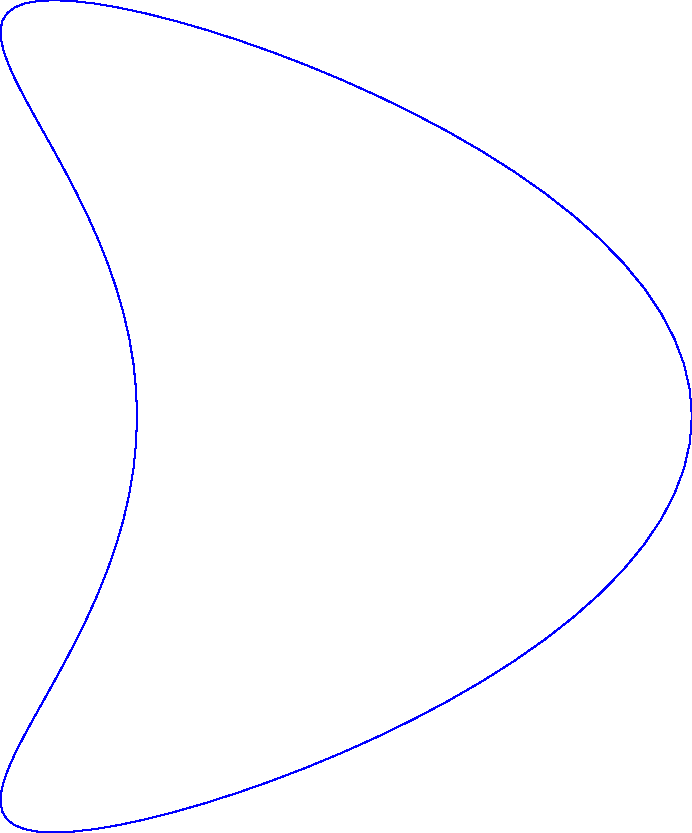
\includegraphics[scale=0.3]{kite.pdf}
  \caption{The ``kite'' domain with boundary $\Gamma = (\cos t + 0.65\cos(2 t) - 0.65, 1.5\sin t)$, $t\in[0, 2\pi]$.}  
\label{fig:kite}
\end{figure}

\section{Direct Problems}
\subsection{Discretization of Integral Equations}

The boundary $\Gamma$ is assumed to be of the $2\pi$ periodic parametric form
\begin{align}\label{eq:boundary}
  z(t) = (z_1(t), z_2(t)),\quad 0\leqslant t\leqslant 2\pi
\end{align}
with
\begin{align}
  (z'_1(t))^2 + (z'_2(t))^2 > 0.
\end{align}
Note that
\begin{subequations}
\begin{align}
  \frac{d\sigma(z(\tau))}{d\tau} &= |z'(\tau)|, \\
  \nu(z(\tau)) &= \frac{1}{|z'(\tau)|}(z'_2(\tau), -z'_1(\tau)).
\end{align}
\end{subequations}
By means of the periodic boundary representation \eqref{eq:boundary}, boundary integral operators on $\Gamma$ of the form
\begin{align*}
  \int_\Gamma f(x, y)g(y)\,\text{d}\sigma(y), \quad x\in\Gamma
\end{align*}
with kernel $f$ and operand $g$ will be transformed into
\begin{align*}
  \int_0^{2\pi} f(z(t), z(\tau))g(z(\tau))|z'(\tau)|\,\text{d}\tau, \quad 0\leqslant t\leqslant 2\pi.
\end{align*}
\begin{align}
  H_n^1(z) = J_n(z) + i\,Y_n(z)
\end{align}

\begin{equation}
\begin{split}
  Y_0(z) &= \frac{2}{\pi}\left(\gamma + \ln\left(\frac{z}{2}\right)\right)J_0(z)-\frac{4}{\pi}\sum_{j=0}^\infty\frac{(-1)^j}{j}J_{2j}(z) \\
  Y_1(z) &= -\frac{2}{\pi z}J_0(z) + \frac{2}{\pi}\left(\ln\left(\frac{z}{2}\right) + \gamma-1\right)J_1(z)-\frac{2}{\pi}\sum_{j=1}^\infty\frac{(-1)^j(2j+1)}{j(j+1)}J_{2j+1}(z)
\end{split}
\end{equation}

\begin{equation}
\begin{split}
  \left(\widetilde{T}_k\varphi\right)(x) &= (T_k\varphi)(x)-(T_0\varphi)(x) \\
  &= \frac{\partial}{\partial\nu(x)}\ints{\frac{\partial}{\partial\nu(y)}\left\{\frac{i}{2}H_0^1(k|x-y|) + \frac{1}{\pi}\ln|x-y|\right\}\varphi(y)}(y)
\end{split}
\end{equation}

\begin{subequations}
\begin{align}
  S_k\varphi(t) &= \int_0^{2\pi}{\sf M}_k(t,\tau)\varphi(\tau)\,d\tau \\
  K_k\varphi(t) &= \int_0^{2\pi}{\sf L}_k(t,\tau)\varphi(\tau)\,d\tau \\
  K^*_k\varphi(t) &= \int_0^{2\pi}{\sf L}_k^*(t,\tau)\varphi(\tau)\,d\tau \\
  \widetilde{T}_k\varphi(t) &= \int_0^{2\pi}{\sf N}_k(t,\tau)\varphi(\tau)\,d\tau 
\end{align}
\end{subequations}

With
\begin{align}
  r(t,\tau)=\left\{\left(z_1(t)-z_1(\tau)\right)^2 + \left(z_2(t)-z_2(\tau)\right)^2 \right\}^{\frac{1}{2}},
\end{align}
we have
\begin{subequations}
\begin{align}
  {\sf M}_k(t,\tau) &= \frac{i}{2}H_0^1(kr(t,\tau))|z'(\tau)|\\
  {\sf L}_k(t,\tau) &= \frac{ik}{2}\left\{z'_2(\tau)[z_1(t)-z_1(\tau)]-z'_1(\tau)[z_2(t)-z_2(\tau)]\right\}\frac{H_1^1(kr(t,\tau))}{r(t,\tau)} \\
  {\sf L}_k^*(t,\tau) &= -\frac{ik}{2}\left\{z'_2(t)[z_1(t)-z_1(\tau)]-z'_1(t)[z_2(t)-z_2(\tau)]\right\}\frac{|z'(\tau)|}{|z'(t)|}\frac{H_1^1(kr(t,\tau))}{r(t,\tau)} \\
  &= \frac{|z'(\tau)|}{|z'(t)|} {\sf L}_k(\tau, t) \\
  {\sf N}_k(t, \tau) &= \left\{z'_2(t)[z_1(t)-z_1(\tau)]-z'_1(t)[z_2(t)-z_2(\tau)]\right\}\\
  &\times\left\{z'_2(\tau)[z_1(t)-z_1(\tau)]-z'_1(\tau)[z_2(t)-z_2(\tau)]\right\}\notag \\
  &\times\frac{1}{|z'(t)|r(t, \tau)^4}\left\{\frac{ik^2}{2}H_0^1(kr(t,\tau))r(t,\tau)^2-ikH_1^1(kr(t,\tau))r(t,\tau)+\frac{2}{\pi}\right\}\notag \\
  &+\frac{z'_1(t)z'_1(\tau)+z'_2(t)z'_2(\tau)}{|z'(t)|r(t,\tau)^2}\left\{\frac{ik}{2}H_1^1(kr(t,\tau))r(t,\tau)-\frac{1}{\pi}\right\}\notag
\end{align}
\end{subequations}

\begin{subequations}
\begin{align}
  H_0^1(z) &= \frac{2i}{\pi}\ln\left(\frac{z}{2}\right)\,J_0(z) + \cdots \\
  H_1^1(z) &= \frac{2i}{\pi}\ln\left(\frac{z}{2}\right)\,J_1(z) + \cdots \\
  \ln\frac{z}{2} &= \ln\left(\frac{kr(t,\tau)}{4|\sin\frac{(t-\tau)}{2}|}\right) + \frac{1}{2}\ln\left(4\sin^2\frac{t-\tau}{2}\right) + \cdots
\end{align}
\end{subequations}

\begin{subequations}
\begin{align}
  {\sf M}_k(t, \tau) &= {\sf M}_k^1(t, \tau)\ln\left(4\sin^2\frac{t-\tau}{2}\right) + {\sf M}_k^2(t, \tau) \\
  {\sf L}_k(t, \tau) &= {\sf L}_k^1(t, \tau)\ln\left(4\sin^2\frac{t-\tau}{2}\right) + {\sf L}_k^2(t, \tau) \\
  {\sf L}_k^*(t, \tau) &= {\sf L}_k^{*1}(t, \tau)\ln\left(4\sin^2\frac{t-\tau}{2}\right) + {\sf L}_k^{*2}(t, \tau) \\
  {\sf N}_k(t, \tau) &= {\sf N}_k^1(t, \tau)\ln\left(4\sin^2\frac{t-\tau}{2}\right) + {\sf N}_k^2(t, \tau) 
\end{align}
\end{subequations}

\begin{subequations}
\begin{align}
  {\sf M}_k^1(t,\tau) &= -\frac{1}{2\pi}J_0(kr(t,\tau))|z'(\tau)| \\
  {\sf M}_k^2(t,\tau) &= {\sf M}_k(t,\tau) - {\sf M}_k^1(t,\tau)\ln\left(4\sin^2\frac{t-\tau}{2}\right) \\
  {\sf L}_k^1(t,\tau) &= -\frac{k}{2\pi}\left\{z'_2(\tau)[z_1(t)-z_1(\tau)]-z'_1(\tau)[z_2(t)-z_2(\tau)]\right\}\frac{J_1(kr(t,\tau))}{r(t,\tau)} \\
  {\sf L}_k^2(t,\tau) &= {\sf L}_k(t,\tau) - {\sf L}_k^1(t,\tau)\ln\left(4\sin^2\frac{t-\tau}{2}\right) \\
  {\sf L}_k^{*1}(t,\tau) &= \frac{|z'(\tau)|}{|z'(t)|}L_k^1(t,\tau) \\
  {\sf L}_k^{*2}(t,\tau) &= {\sf L}_k^*(t,\tau) - {\sf L}_k^{*1}(t,\tau)\ln\left(4\sin^2\frac{t-\tau}{2}\right) \\
  &= \frac{|z'(\tau)|}{|z'(t)|}{\sf L}_k^2(t,\tau)\notag\\
  {\sf N}_k^1(t,\tau) =& \left\{z'_2(t)[z_1(t)-z_1(\tau)]-z'_1(t)[z_2(t)-z_2(\tau)]\right\}\notag \\
  &\times\left\{z'_2(\tau)[z_1(t)-z_1(\tau)]-z'_1(\tau)[z_2(t)-z_2(\tau)]\right\}\notag\\
  &\times\frac{1}{|z'(t)|r(t, \tau)^4}\left\{-\frac{k^2}{2\pi}J_0(kr(t,\tau))r(t,\tau)^2+\frac{k}{\pi}J_1(kr(t,\tau))r(t,\tau)\right\}\notag \\
  &-\frac{k}{2\pi}\frac{z'_1(t)z'_1(\tau)+z'_2(t)z'_2(\tau)}{|z'(t)|r(t,\tau)^2}J_1(kr(t,\tau))\notag \\
  {\sf N}_k^2(t,\tau) =& {\sf N}_k(t,\tau) - {\sf N}_k^1(t,\tau)\ln\left(4\sin^2\frac{t-\tau}{2}\right) 
\end{align}
\end{subequations}

\begin{subequations}
\begin{align}
  {\sf M}_k^1(t,t) &= -\frac{1}{2\pi}|z'(\tau)| \\
  {\sf M}_k^2(t,t) &= |z'(t)|\left\{\frac{i}{2}-\frac{\gamma}{\pi}-\frac{1}{2\pi}\ln\frac{k^2|z'(t)|^2}{4}\right\} \\
  {\sf L}_k^1(t,t) &= 0 \\
  {\sf L}_k^2(t,t) &= -\frac{1}{2\pi}\frac{z'_1(t)z''_2(t)-z'_2(t)z''_1(t)}{|z'(t)^2|} \\
  {\sf L}_k^{*1}(t,t) &= 0 \\
  {\sf L}_k^{*2}(t,t) &= {\sf L}_k^2(t,t) \\
  {\sf N}_k^1(t,t) &= -\frac{k^2}{4\pi}|z'(t)|\\ 
  {\sf N}_k^2(t,t) &= \frac{k^2}{2}\left\{\frac{i}{2}-\frac{\gamma}{\pi}-\frac{1}{2\pi}\ln\frac{k^2|z'(t)|^2}{4}+\frac{1}{2\pi}\right\}|z'(t)| 
\end{align}
\end{subequations}

\begin{align}
  \int_0^{2\pi}\ln\left(4\sin^2\frac{t-\tau}{2}\right)f(\tau)\,d\tau\approx\sum_{j=0}^{2n-1}R^{(n)}_j(t)f(t_j),\quad 0\leqslant t\leqslant 2\pi
\end{align}

$$t_j=\frac{\pi j}{n},\quad j=0,\cdots,2n-1$$

\begin{align}
  R^{(n)}_j(t) = -\frac{2\pi}{n}\sum_{l=1}^{n-1}\frac{1}{l}\cos\left(l(t-t_j)\right)-\frac{\pi}{n^2}\cos\left(n(t-t_j)\right), \quad j=0,\cdots,2n-1
\end{align}

\begin{align}
  \int_0^{2\pi}f(\tau)\,d\tau\approx\frac{\pi}{n}\sum_{j=0}^{2n-1}f(t_j)
\end{align}

\begin{align}
  E\psi^{(n)}(t) + \sum_{j=0}^{2n-1}\left\{R^{(n)}_j(t)A^1(t, t_j) + \frac{\pi}{n}A^2(t, t_j)\right\}\psi^{(n)}(t_j) = u(t), \quad 0\leqslant t\leqslant 2\pi
\end{align}

\begin{align}
  \psi_i^{(n)} &:= \psi^{(n)}(t_i),\quad i=0,\cdots,2n-1 \\
  R^{(n)}_{|i-j|} &:= R^{(n)}_j(t_i) 
\end{align}

\begin{align}
  E\psi_i^{(n)} + \sum_{j=0}^{2n-1}\left\{R^{(n)}_{|i-j|}A^1(t_i, t_j) + \frac{\pi}{n}A^2(t_i, t_j)\right\}\psi_j^{(n)} = u(t_i),\quad i=0,\cdots,2n-1 
\end{align}

\begin{align}
  R^{(n)}_l = R^{(n)}_l(0) = -\frac{2\pi}{n}\sum_{m=1}^{n-1}\frac{1}{m}\cos\frac{ml\pi}{n}-\frac{(-1)^l\pi}{n^2},\quad j=0,\cdots,2n-1
\end{align}

\begin{align}
  &Q_\text{er}^\infty(\hat x)\notag \\
  &= \frac{e^{-\frac{i\pi}{4}}}{\sqrt{8\pi\gamma_\text{er}}}\int_0^{2\pi}\left\{\gamma_\text{er}[\hat{x_1}z'_2(\tau)-\hat{x_2}z'_1(\tau)]\psi_3(\tau)+ic_1|z'(\tau)|\psi_1(\tau)\right\}e^{-i\gamma_\text{er}(\hat{x_1}z_1(\tau)+\hat{x_2}z_2(\tau))}\,d\tau\notag \\
  &= \frac{e^{-\frac{i\pi}{4}}}{\sqrt{8\pi\gamma_\text{er}}}\frac{\pi}{n}\sum_{j=0}^{2n-1}\left\{\gamma_\text{er}[\hat{x_1}z'_2(t_j)-\hat{x_2}z'_1(t_j)]\psi^{(n)}_{j;3}+ic_1|z'(t_j)|\psi^{(n)}_{j;1}(t_j)\right\}e^{-i\gamma_\text{er}(\hat{x_1}z_1(t_j)+\hat{x_2}z_2(t_j))}
\end{align}

\begin{align}
  &Q_\text{el}^\infty(\hat x)\notag \\
  &= \frac{e^{-\frac{i\pi}{4}}}{\sqrt{8\pi\gamma_\text{el}}}\int_0^{2\pi}\left\{\gamma_\text{el}[\hat{x_1}z'_2(\tau)-\hat{x_2}z'_1(\tau)]\psi_4(\tau)+ic_1|z'(\tau)|\psi_2(\tau)\right\}e^{-i\gamma_\text{el}(\hat{x_1}z_1(\tau)+\hat{x_2}z_2(\tau))}\,d\tau\notag \\
  &= \frac{e^{-\frac{i\pi}{4}}}{\sqrt{8\pi\gamma_\text{el}}}\frac{\pi}{n}\sum_{j=0}^{2n-1}\left\{\gamma_\text{el}[\hat{x_1}z'_2(t_j)-\hat{x_2}z'_1(t_j)]\psi^{(n)}_{j;4}+ic_1|z'(t_j)|\psi^{(n)}_{j;2}(t_j)\right\}e^{-i\gamma_\text{el}(\hat{x_1}z_1(t_j)+\hat{x_2}z_2(t_j))}
\end{align}

\subsection{Calibration}

Note that if
\begin{align*}
  Q_1 &= c_1 J_0(k_1 |x|) \\
  Q_2 &= c_2 H_0^1(k_2 |x|) \\
\end{align*}
then
\begin{align*}
  \frac{\partial Q_1}{\partial\nu} &= -k_1 c_1 J_1(k_1|x|)\,\nu(x)\cdot\frac{x}{|x|}\\
  \frac{\partial Q_2}{\partial\nu} &= -k_2 c_2 H_1^1(k_2|x|)\,\nu(x)\cdot\frac{x}{|x|}\\
\end{align*}

\subsubsection{Chiral-Chiral}

The boundary terms according to ``master equations'' are
\begin{align*}
  u_1 &= \delta(Q_\text{ir} + Q_\text{il}) - (Q_\text{er} + Q_\text{el})\\
  u_2 &= i\rho(Q_\text{ir} - Q_\text{il}) -i(Q_\text{er} - Q_\text{el}) \\
  u_3 &=\delta\left(\frac{1}{\gamma_\text{ir}}\frac{\partial Q_\text{ir}}{\partial\nu} - \frac{1}{\gamma_\text{il}}\frac{\partial Q_\text{il}}{\partial\nu}\right) -\left(\frac{1}{\gamma_\text{er}}\frac{\partial Q_\text{er}}{\partial\nu} - \frac{1}{\gamma_\text{el}}\frac{\partial Q_\text{el}}{\partial\nu}\right) \\
  u_4 &=i\rho\left(\frac{1}{\gamma_\text{ir}}\frac{\partial Q_\text{ir}}{\partial\nu} + \frac{1}{\gamma_\text{il}}\frac{\partial Q_\text{il}}{\partial\nu}\right) -i\left(\frac{1}{\gamma_\text{er}}\frac{\partial Q_\text{er}}{\partial\nu} + \frac{1}{\gamma_\text{el}}\frac{\partial Q_\text{el}}{\partial\nu}\right) \\
\end{align*}
Given the fields
\begin{align*}
  Q_\text{er} &= c_\text{er}H_0^1(\gamma_\text{er}\,|x|) \\
  Q_\text{el} &= c_\text{el}H_0^1(\gamma_\text{el}\,|x|) \\
  Q_\text{ir} &= c_\text{ir}J_0(\gamma_\text{ir}\,|x|) \\
  Q_\text{il} &= c_\text{il}J_0(\gamma_\text{il}\,|x|)
\end{align*}
where $c_i$'s are constants, we have
\begin{align*}
  u_1 &= c_\text{ir} \delta J_0(\gamma_\text{ir}|x|)+c_\text{il} \delta J_0(\gamma_\text{il}|x|)-c_\text{er} H_0^1(\gamma_\text{er}|x|)-c_\text{el} H_0^1(\gamma_\text{el}|x|) \\
  u_2 &= i \bigl(c_\text{ir} J_0(\gamma_\text{ir}|x|) \rho-c_\text{il} J_0(\gamma_\text{il}|x|) \rho-c_\text{er} H_0^1(\gamma_\text{er}|x|)+c_\text{el} H_0^1(\gamma_\text{el}|x|)\bigr) \\
  u_3 &= -\nu(x)\cdot\frac{x}{|x|} \bigl(c_\text{ir} \delta J_1(\gamma_\text{ir}|x|)-c_\text{il} \delta J_1(\gamma_\text{il}|x|)-c_\text{er} H_1^1(\gamma_\text{er}|x|)+c_\text{el} H_1^1(\gamma_\text{el}|x|)\bigr) \\
  u_4 &= -i \nu(x)\cdot\frac{x}{|x|} \bigl(c_\text{ir} J_1(\gamma_\text{ir}|x|) \rho+c_\text{il} J_1(\gamma_\text{il}|x|) \rho-c_\text{er} H_1^1(\gamma_\text{er}|x|)-c_\text{el} H_1^1(\gamma_\text{el}|x|)\bigr) \\
\end{align*}

\subsubsection{Achiral-Chiral}

The boundary terms according to ``master equations'' are
\begin{align*}
  u_1 &= \delta(Q_\text{ir} + Q_\text{il}) - (Q_\text{er} + Q_\text{el})\\
  u_2 &= i\rho(Q_\text{ir} - Q_\text{il}) -i(Q_\text{er} - Q_\text{el}) \\
  u_3 &=\delta\left(\frac{1}{\gamma_\text{ir}}\frac{\partial Q_\text{ir}}{\partial\nu} - \frac{1}{\gamma_\text{il}}\frac{\partial Q_\text{il}}{\partial\nu}\right) -\left(\frac{1}{k_\text{e}}\frac{\partial Q_\text{er}}{\partial\nu} - \frac{1}{k_\text{e}}\frac{\partial Q_\text{el}}{\partial\nu}\right) \\
  u_4 &=i\rho\left(\frac{1}{\gamma_\text{ir}}\frac{\partial Q_\text{ir}}{\partial\nu} + \frac{1}{\gamma_\text{il}}\frac{\partial Q_\text{il}}{\partial\nu}\right) -i\left(\frac{1}{k_\text{e}}\frac{\partial Q_\text{er}}{\partial\nu} + \frac{1}{k_\text{e}}\frac{\partial Q_\text{el}}{\partial\nu}\right) \\
\end{align*}
Given the fields
\begin{align*}
  Q_\text{er} &= c_\text{er}H_0^1(k_\text{e}|x|) \\
  Q_\text{el} &= c_\text{el}H_0^1(k_\text{e}|x|) \\
  Q_\text{ir} &= c_\text{ir}J_0(\gamma_\text{ir}|x|) \\
  Q_\text{il} &= c_\text{il}J_0(\gamma_\text{il}|x|)
\end{align*}
where $c_i$'s are constants, we have
\begin{align*}
  u_1 &= c_\text{ir} \delta J_0(\gamma_\text{ir}|x|)+c_\text{il} \delta J_0(\gamma_\text{il}|x|)-c_\text{er} H_0^1(k_\text{e}|x|)-c_\text{el} H_0^1(k_\text{e}|x|)\\
  u_2 &= i \bigl(c_\text{ir} J_0(\gamma_\text{ir}|x|) \rho-c_\text{il} J_0(\gamma_\text{il}|x|) \rho-c_\text{er} H_0^1(k_\text{e}|x|)+c_\text{el} H_0^1(k_\text{e}|x|)\bigr)\\
  u_3 &=-\nu(x)\cdot\frac{x}{|x|} \bigl(c_\text{ir} \delta J_1(\gamma_\text{ir}|x|)-c_\text{il} \delta J_1(\gamma_\text{il}|x|)-c_\text{er} H_1^1(k_\text{e}|x|)+c_\text{el} H_1^1(k_\text{e}|x|)\bigr) \\
  u_4 &=-i \nu(x)\cdot\frac{x}{|x|} \bigl(c_\text{ir} J_1(\gamma_\text{ir}|x|) \rho+c_\text{il} J_1(\gamma_\text{il}|x|) \rho-c_\text{er} H_1^1(k_\text{e}|x|)-c_\text{el} H_1^1(k_\text{e}|x|)\bigr)\\
\end{align*}

\subsubsection{Chiral-Achiral}

The boundary terms according to ``master equations'' are
\begin{align*}
  u_1 &= \delta(Q_\text{ir} + Q_\text{il}) - (Q_\text{er} + Q_\text{el})\\
  u_2 &= i\rho(Q_\text{ir} - Q_\text{il}) -i(Q_\text{er} - Q_\text{el}) \\
  u_3 &=\delta\left(\frac{1}{k_\text{i}}\frac{\partial Q_\text{ir}}{\partial\nu} - \frac{1}{k_\text{i}}\frac{\partial Q_\text{il}}{\partial\nu}\right) -\left(\frac{1}{\gamma_\text{er}}\frac{\partial Q_\text{er}}{\partial\nu} - \frac{1}{\gamma_\text{el}}\frac{\partial Q_\text{el}}{\partial\nu}\right) \\
  u_4 &=i\rho\left(\frac{1}{k_\text{i}}\frac{\partial Q_\text{ir}}{\partial\nu} + \frac{1}{k_\text{i}}\frac{\partial Q_\text{il}}{\partial\nu}\right) -i\left(\frac{1}{\gamma_\text{er}}\frac{\partial Q_\text{er}}{\partial\nu} + \frac{1}{\gamma_\text{el}}\frac{\partial Q_\text{el}}{\partial\nu}\right) \\
\end{align*}
Given the fields
\begin{align*}
  Q_\text{er} &= c_\text{er}H_0^1(\gamma_\text{er}|x|) \\
  Q_\text{el} &= c_\text{el}H_0^1(\gamma_\text{el}|x|) \\
  Q_\text{ir} &= c_\text{ir}J_0(k_\text{i}|x|) \\
  Q_\text{il} &= c_\text{il}J_0(k_\text{i}|x|)
\end{align*}
where $c_i$'s are constants, we have
\begin{align*}
  u_1 &= c_\text{ir} \delta J_0(k_\text{i}|x|)+c_\text{il} \delta J_0(k_\text{i}|x|)-c_\text{er} H_0^1(\gamma_\text{er}|x|)-c_\text{el} H_0^1(\gamma_\text{el}|x|) \\
  u_2 &= i \bigl(c_\text{ir} J_0(k_\text{i}|x|) \rho-c_\text{il} J_0(k_\text{i}|x|) \rho-c_\text{er} H_0^1(\gamma_\text{er}|x|)+c_\text{el} H_0^1(\gamma_\text{el}|x|)\bigr)\\
  u_3 &= -\nu(x)\cdot\frac{x}{|x|} \bigl(c_\text{ir} \delta J_1(k_\text{i}|x|)-c_\text{il} \delta J_1(k_\text{i}|x|)-c_\text{er} H_1^1(\gamma_\text{er}|x|)+c_\text{el} H_1^1(\gamma_\text{el}|x|)\bigr)\\
  u_4 &= -i \nu(x)\cdot\frac{x}{|x|} \bigl(c_\text{ir} J_1(k_\text{i}|x|) \rho+c_\text{il} J_1(k_\text{i}|x|) \rho-c_\text{er} H_1^1(\gamma_\text{er}|x|)-c_\text{el} H_1^1(\gamma_\text{el}|x|)\bigr) \\
\end{align*}

\subsubsection{Chiral-Perfect Conductor}

The boundary terms according to ``master equations'' are
\begin{align*}
  u_1 &= -i(Q_\text{er} - Q_\text{el}) \\
  u_2 &= -i\left(\frac{1}{\gamma_\text{er}}\frac{\partial Q_\text{er}}{\partial\nu} + \frac{1}{\gamma_\text{el}}\frac{\partial Q_\text{el}}{\partial\nu}\right) \\
\end{align*}
Given the fields
\begin{align*}
  Q_\text{er} &= c_\text{er}H_0^1(\gamma_\text{er}|x|) \\
  Q_\text{el} &= c_\text{el}H_0^1(\gamma_\text{el}|x|)
\end{align*}
where $c_i$'s are constants, we have
\begin{align*}
  u_1 &= -i \bigl(c_\text{er} H_0^1(\gamma_\text{er}|x|)-c_\text{el} H_0^1(\gamma_\text{el}|x|)\bigr) \\
  u_2 &= i \nu(x)\cdot\frac{x}{|x|} \bigl(c_\text{er} H_1^1(\gamma_\text{er}|x|)+c_\text{el} H_1^1(\gamma_\text{el}|x|)\bigr)
\end{align*}

\subsection{Calibration Results}

\begin{table*}
  \centering
  \renewcommand{\arraystretch}{1.1}
  \caption{Parameters Used in Calibration}
  \begin{tabular}{@{}ccccc@{}}
    \toprule
    parameter  & chiral-chiral & chiral-achiral & achiral-chiral & chiral-perfect conductor \\ 
    \midrule
    $c_\text{il}$ & $1+i$ & $1+i$ & $1+i$ & ---\\
    $c_\text{ir}$ & $2i$ & 3 & 3 & ---\\
    $c_\text{el}$ & $1-0.5i$ & 1 & 1 & 1\\
    $c_\text{er}$ & $2$ & 2 & 2 & 2\\
    $\varepsilon_\text{i}$ & 1.4 & 1.4 & 1.4 & ---\\
    $\mu_\text{i}$ & 1.2 & 1.2 & 1.2 & ---\\
    $\beta_\text{i}$ & 0.1 & 0 & 0.1 & ---\\
    $\varepsilon_\text{e}$ & 1.3 & 1.1 & 1 & 1.4\\
    $\mu_\text{e}$ & 1.25 & 1.15 & 1 & 1.2\\
    $\beta_\text{e}$ & 0.05 & 0.05 & 0 & 0.1\\
    \bottomrule
  \end{tabular}
\end{table*}

\begin{table*}
  \centering
  \renewcommand{\arraystretch}{1.1}
  \caption{$Q_\text{el}^\infty$, Chiral-Chiral, $\omega=1$}
  \begin{tabular}{@{}llll@{}}
    \toprule
    n & $\Re{Q_\text{el}^\infty}$ & $\Im{Q_\text{el}^\infty}$ & error \\
    \midrule
8 & 0.243508249431 & -0.724463645911 & 0.00252276843633\\ 
16 & 0.241757267708 & -0.725273624079 & 7.57632109346e-07\\ 
32 & 0.241757794244 & -0.725273382729 & 1.30143110535e-12\\ 
64 & 0.241757794243 & -0.72527338273 & 7.48452457873e-16\\ 
128 & 0.241757794243 & -0.72527338273 & ---\\%8.66015942639e-16\\ 
    \bottomrule
  \end{tabular}
  \\ 
  $$\text{exact }\Re{Q_\text{el}^\infty}=0.241757794243,\,\Im{Q_\text{el}^\infty}=-0.72527338273$$  
\end{table*}

\begin{table*}
  \centering
  \renewcommand{\arraystretch}{1.1}
  \caption{$Q_\text{er}^\infty$, Chiral-Chiral, $\omega=1$}
  \begin{tabular}{@{}llll@{}}
    \toprule
    n & $\Re{Q_\text{er}^\infty}$ & $\Im{Q_\text{er}^\infty}$ & error \\
    \midrule
8 & 1.03242377734 & -1.0282192268 & 0.00208410886337\\ 
16 & 1.03076319169 & -1.03076453615 & 7.75447408805e-07\\ 
32 & 1.0307634315 & -1.0307634315 & 1.74692244341e-12\\ 
64 & 1.0307634315 & -1.0307634315 & 5.49209323305e-16\\ 
128 & 1.0307634315 & -1.0307634315 & ---\\%5.49209323305e-16\\ 
    \bottomrule
  \end{tabular}
  \\ 
  $$\text{exact }\Re{Q_\text{er}^\infty}=1.0307634315,\,\Im{Q_\text{er}^\infty}=-1.0307634315$$  
\end{table*}

\begin{table*}
  \centering
  \renewcommand{\arraystretch}{1.1}
  \caption{$Q_\text{el}^\infty$, Chiral-Chiral, $\omega=5$}
  \begin{tabular}{@{}llll@{}}
    \toprule
    n & $\Re{Q_\text{el}^\infty}$ & $\Im{Q_\text{el}^\infty}$ & error \\
    \midrule
8 & -1.54250039 & -0.590088131481 & 5.70708508424\\ 
16 & -1.32334465864 & -0.341629394985 & 4.85869482999\\ 
32 & 0.157231611887 & -0.334208562175 & 0.29760446524\\ 
64 & 0.0922336179119 & -0.27668319242 & 2.26074544743e-05\\ 
128 & 0.0922294278071 & -0.276688283421 & 6.01956349633e-15\\ 
    \bottomrule
  \end{tabular}
  \\ 
  $$\text{exact }\Re{Q_\text{el}^\infty}=0.0922294278071,\,\Im{Q_\text{el}^\infty}=-0.276688283421$$  
\end{table*}

\begin{table*}
  \centering
  \renewcommand{\arraystretch}{1.1}
  \caption{$Q_\text{er}^\infty$, Chiral-Chiral, $\omega=5$}
  \begin{tabular}{@{}llll@{}}
    \toprule
    n & $\Re{Q_\text{er}^\infty}$ & $\Im{Q_\text{er}^\infty}$ & error \\
    \midrule
8 & -0.914018631255 & -1.10274229685 & 2.12747483551\\ 
16 & 0.485271823154 & -0.531252645336 & 0.0458354064657\\ 
32 & 0.514160036173 & -0.514124508444 & 0.00174134854985\\ 
64 & 0.513248314271 & -0.513249251167 & 9.25516228666e-07\\ 
128 & 0.513248703975 & -0.513248703975 & 1.86706958735e-15\\ 
    \bottomrule
  \end{tabular}
  \\ 
  $$\text{exact }\Re{Q_\text{er}^\infty}=0.513248703975,\,\Im{Q_\text{er}^\infty}=-0.513248703975$$  
\end{table*}

\begin{table*}
  \centering
  \renewcommand{\arraystretch}{1.1}
  \caption{$Q_\text{el}^\infty$, Chiral-Achiral, $\omega=1$}
  \begin{tabular}{@{}llll@{}}
    \toprule
    n & $\Re{Q_\text{el}^\infty}$ & $\Im{Q_\text{el}^\infty}$ & error \\
    \midrule
8 & 0.517553169413 & -0.515454523971 & 0.00211709931463\\ 
16 & 0.516813776585 & -0.51681440272 & 8.11410019314e-07\\ 
32 & 0.516813810653 & -0.516813810653 & 1.89097093567e-12\\ 
64 & 0.516813810652 & -0.516813810652 & 3.03802341641e-16\\ 
128 & 0.516813810652 & -0.516813810652 & ---\\ 
    \bottomrule
  \end{tabular}
  \\ 
  $$\text{exact }\Re{Q_\text{el}^\infty}=0.516813810652,\,\Im{Q_\text{el}^\infty}=-0.516813810652$$  
\end{table*}

\begin{table*}
  \centering
  \renewcommand{\arraystretch}{1.1}
  \caption{$Q_\text{er}^\infty$, Chiral-Achiral, $\omega=1$}
  \begin{tabular}{@{}llll@{}}
    \toprule
    n & $\Re{Q_\text{er}^\infty}$ & $\Im{Q_\text{er}^\infty}$ & error \\
    \midrule
8 & 1.09460136497 & -1.09072789032 & 0.00192359535948\\ 
16 & 1.09348494462 & -1.09348581917 & 4.1512146724e-07\\ 
32 & 1.09348526007 & -1.09348526007 & 2.27060990893e-12\\ 
64 & 1.09348526007 & -1.09348526007 & 5.92020513263e-16\\ 
128 & 1.09348526007 & -1.09348526007 & ---\\ 
    \bottomrule
  \end{tabular}
  \\ 
  $$\text{exact }\Re{Q_\text{er}^\infty}=1.09348526007,\,\Im{Q_\text{er}^\infty}=-1.09348526007$$  
\end{table*}

\begin{table*}
  \centering
  \renewcommand{\arraystretch}{1.1}
  \caption{$Q_\text{el}^\infty$, Chiral-Achiral, $\omega=5$}
  \begin{tabular}{@{}llll@{}}
    \toprule
    n & $\Re{Q_\text{el}^\infty}$ & $\Im{Q_\text{el}^\infty}$ & error \\
    \midrule
8 & 0.30026870953 & -0.712558815495 & 1.82383712303\\ 
16 & 0.200579979636 & -0.410772136414 & 0.732891144812\\ 
32 & 0.20170499083 & -0.20171835406 & 3.41968012876e-05\\ 
64 & 0.201709958923 & -0.201709958923 & 3.21233736018e-15\\ 
128 & 0.201709958923 & -0.201709958923 & ---\\%6.61918584537e-15\\ 
    \bottomrule
  \end{tabular}
  \\ 
  $$\text{exact }\Re{Q_\text{el}^\infty}=0.201709958923,\,\Im{Q_\text{el}^\infty}=-0.201709958923$$  
\end{table*}

\begin{table*}
  \centering
  \renewcommand{\arraystretch}{1.1}
  \caption{$Q_\text{er}^\infty$, Chiral-Achiral, $\omega=5$}
  \begin{tabular}{@{}llll@{}}
    \toprule
    n & $\Re{Q_\text{er}^\infty}$ & $\Im{Q_\text{er}^\infty}$ & error \\
    \midrule
8 & -0.20701351838 & -0.109212287124 & 1.12960975313\\ 
16 & 0.547735625223 & -0.536176317021 & 0.0124250415665\\ 
32 & 0.538582690729 & -0.53858241491 & 7.65288725345e-07\\ 
64 & 0.538582941234 & -0.538582941234 & 1.56989871106e-15\\ 
128 & 0.538582941234 & -0.538582941234 & ---\\%1.0306889985e-15\\ 
    \bottomrule
  \end{tabular}
  \\ 
  $$\text{exact }\Re{Q_\text{er}^\infty}=0.538582941234,\,\Im{Q_\text{er}^\infty}=-0.538582941234$$  
\end{table*}

\begin{table*}
  \centering
  \renewcommand{\arraystretch}{1.1}
  \caption{$Q_\text{el}^\infty$, Achiral-Chiral, $\omega=1$}
  \begin{tabular}{@{}llll@{}}
    \toprule
    n & $\Re{Q_\text{el}^\infty}$ & $\Im{Q_\text{el}^\infty}$ & error \\
    \midrule
8 & 0.564621897758 & -0.562665174455 & 0.00198590726036\\ 
16 & 0.564189380256 & -0.564189852447 & 4.22488162925e-07\\ 
32 & 0.564189583547 & -0.564189583545 & 3.02452614006e-12\\ 
64 & 0.564189583548 & -0.564189583548 & 1.12182947538e-15\\ 
128 & 0.564189583548 & -0.564189583548 & ---\\ 
    \bottomrule
  \end{tabular}
  \\ 
  $$\text{exact }\Re{Q_\text{el}^\infty}=0.564189583548,\,\Im{Q_\text{el}^\infty}=-0.564189583548$$  
\end{table*}

\begin{table*}
  \centering
  \renewcommand{\arraystretch}{1.1}
  \caption{$Q_\text{er}^\infty$, Achiral-Chiral, $\omega=1$}
  \begin{tabular}{@{}llll@{}}
    \toprule
    n & $\Re{Q_\text{er}^\infty}$ & $\Im{Q_\text{er}^\infty}$ & error \\
    \midrule
8 & 1.12939682663 & -1.12573323433 & 0.00177650273147\\ 
16 & 1.12837893453 & -1.12837995564 & 5.15193216419e-07\\ 
32 & 1.12837916709 & -1.12837916709 & 2.01395207188e-12\\ 
64 & 1.1283791671 & -1.1283791671 & 4.40017721993e-16\\ 
128 & 1.1283791671 & -1.1283791671 & ---\\ 
    \bottomrule
  \end{tabular}
  \\ 
  $$\text{exact }\Re{Q_\text{er}^\infty}=1.1283791671,\,\Im{Q_\text{er}^\infty}=-1.1283791671$$  
\end{table*}

\begin{table*}
  \centering
  \renewcommand{\arraystretch}{1.1}
  \caption{$Q_\text{el}^\infty$, Achiral-Chiral, $\omega=5$}
  \begin{tabular}{@{}llll@{}}
    \toprule
    n & $\Re{Q_\text{el}^\infty}$ & $\Im{Q_\text{el}^\infty}$ & error \\
    \midrule
8 & -1.38080129148 & -1.2059316398 & 5.29994165852\\ 
16 & -0.176692628905 & -0.350908885116 & 1.23363025131\\ 
32 & 0.2768771934 & -0.182011193168 & 0.208701580971\\ 
64 & 0.252325246554 & -0.252321699817 & 4.11143070506e-05\\ 
128 & 0.252313252202 & -0.252313252202 & 3.45420918345e-15\\ 
    \bottomrule
  \end{tabular}
  \\ 
  $$\text{exact }\Re{Q_\text{el}^\infty}=0.252313252202,\,\Im{Q_\text{el}^\infty}=-0.252313252202$$  
\end{table*}

\begin{table*}
  \centering
  \renewcommand{\arraystretch}{1.1}
  \caption{$Q_\text{er}^\infty$, Achiral-Chiral, $\omega=5$}
  \begin{tabular}{@{}llll@{}}
    \toprule
    n & $\Re{Q_\text{er}^\infty}$ & $\Im{Q_\text{er}^\infty}$ & error \\
    \midrule
8 & -0.283950058348 & -0.305333620019 & 1.13973283355\\ 
16 & 0.495725962103 & -0.501971233041 & 0.0130150291233\\ 
32 & 0.503544847795 & -0.505898206999 & 0.00233937408589\\ 
64 & 0.504625161441 & -0.504626766172 & 1.91723918982e-06\\ 
128 & 0.504626504404 & -0.504626504404 & 2.11597746912e-15\\ 
    \bottomrule
  \end{tabular}
  \\ 
  $$\text{exact }\Re{Q_\text{er}^\infty}=0.504626504404,\,\Im{Q_\text{er}^\infty}=-0.504626504404$$  
\end{table*}

\begin{table*}
  \centering
  \renewcommand{\arraystretch}{1.1}
  \caption{$Q_\text{el}^\infty$, Chiral-Perfect Conductor, $\omega=1$}
  \begin{tabular}{@{}llll@{}}
    \toprule
    n & $\Re{Q_\text{el}^\infty}$ & $\Im{Q_\text{el}^\infty}$ & error \\
    \midrule
8 & 0.463559211052 & -0.460881978899 & 0.00290528086333\\ 
16 & 0.462330209434 & -0.462330386333 & 2.61720255786e-06\\ 
32 & 0.462331504632 & -0.462331504679 & 5.35048489119e-11\\ 
64 & 0.462331504662 & -0.462331504662 & 6.1222832642e-16\\ 
128 & 0.462331504662 & -0.462331504662 & ---\\%4.24503966e-16\\ 
    \bottomrule
  \end{tabular}
  \\ 
  $$\text{exact }\Re{Q_\text{el}^\infty}=0.462331504662,\,\Im{Q_\text{el}^\infty}=-0.462331504662$$  
\end{table*}

\begin{table*}
  \centering
  \renewcommand{\arraystretch}{1.1}
  \caption{$Q_\text{er}^\infty$, Chiral-Perfect Conductor, $\omega=1$}
  \begin{tabular}{@{}llll@{}}
    \toprule
    n & $\Re{Q_\text{er}^\infty}$ & $\Im{Q_\text{er}^\infty}$ & error \\
    \midrule
8 & 1.05517487942 & -1.05108924213 & 0.00195575830377\\ 
16 & 1.05339681853 & -1.05340126998 & 2.11298904147e-06\\ 
32 & 1.05339906484 & -1.05339906484 & 2.14225596584e-11\\ 
64 & 1.05339906482 & -1.05339906482 & 4.71337831248e-16\\ 
128 & 1.05339906482 & -1.05339906482 & ---\\%6.6657235341e-16\\ 
    \bottomrule
  \end{tabular}
  \\ 
  $$\text{exact }\Re{Q_\text{er}^\infty}=1.05339906482,\,\Im{Q_\text{er}^\infty}=-1.05339906482$$  
\end{table*}

\begin{table*}
  \centering
  \renewcommand{\arraystretch}{1.1}
  \caption{$Q_\text{el}^\infty$, Chiral-Perfect Conductor, $\omega=5$}
  \begin{tabular}{@{}llll@{}}
    \toprule
    n & $\Re{Q_\text{el}^\infty}$ & $\Im{Q_\text{el}^\infty}$ & error \\
    \midrule
8 & -1.3859292999 & -2.36655602671 & 14.529533948\\ 
16 & 1.18976771222 & -1.24398483508 & 8.25824844059\\ 
32 & 0.151186067614 & 0.157450832994 & 1.55754026122\\ 
64 & 0.132779683355 & -0.132115233073 & 0.00782681251132\\ 
128 & 0.131473545422 & -0.131473545422 & 9.09496118187e-15\\ 
    \bottomrule
  \end{tabular}
  \\ 
  $$\text{exact }\Re{Q_\text{el}^\infty}=0.131473545422,\,\Im{Q_\text{el}^\infty}=-0.131473545422$$  
\end{table*}

\begin{table*}
  \centering
  \renewcommand{\arraystretch}{1.1}
  \caption{$Q_\text{er}^\infty$, Chiral-Perfect Conductor, $\omega=5$}
  \begin{tabular}{@{}llll@{}}
    \toprule
    n & $\Re{Q_\text{er}^\infty}$ & $\Im{Q_\text{er}^\infty}$ & error \\
    \midrule
8 & -0.0113788027834 & 1.58425059547 & 2.77129864916\\ 
16 & 0.509670739085 & -0.617842449859 & 0.0954999201488\\ 
32 & 0.572425660343 & -0.579442075825 & 0.0136177506068\\ 
64 & 0.5690246566 & -0.569024880861 & 2.56074083006e-07\\ 
128 & 0.569024675678 & -0.569024675678 & 1.00438927556e-15\\ 
    \bottomrule
  \end{tabular}
  \\ 
  $$\text{exact }\Re{Q_\text{er}^\infty}=0.569024675678,\,\Im{Q_\text{er}^\infty}=-0.569024675678$$  
\end{table*}

\section{Inverse Problem}

\begin{figure}
\centering
  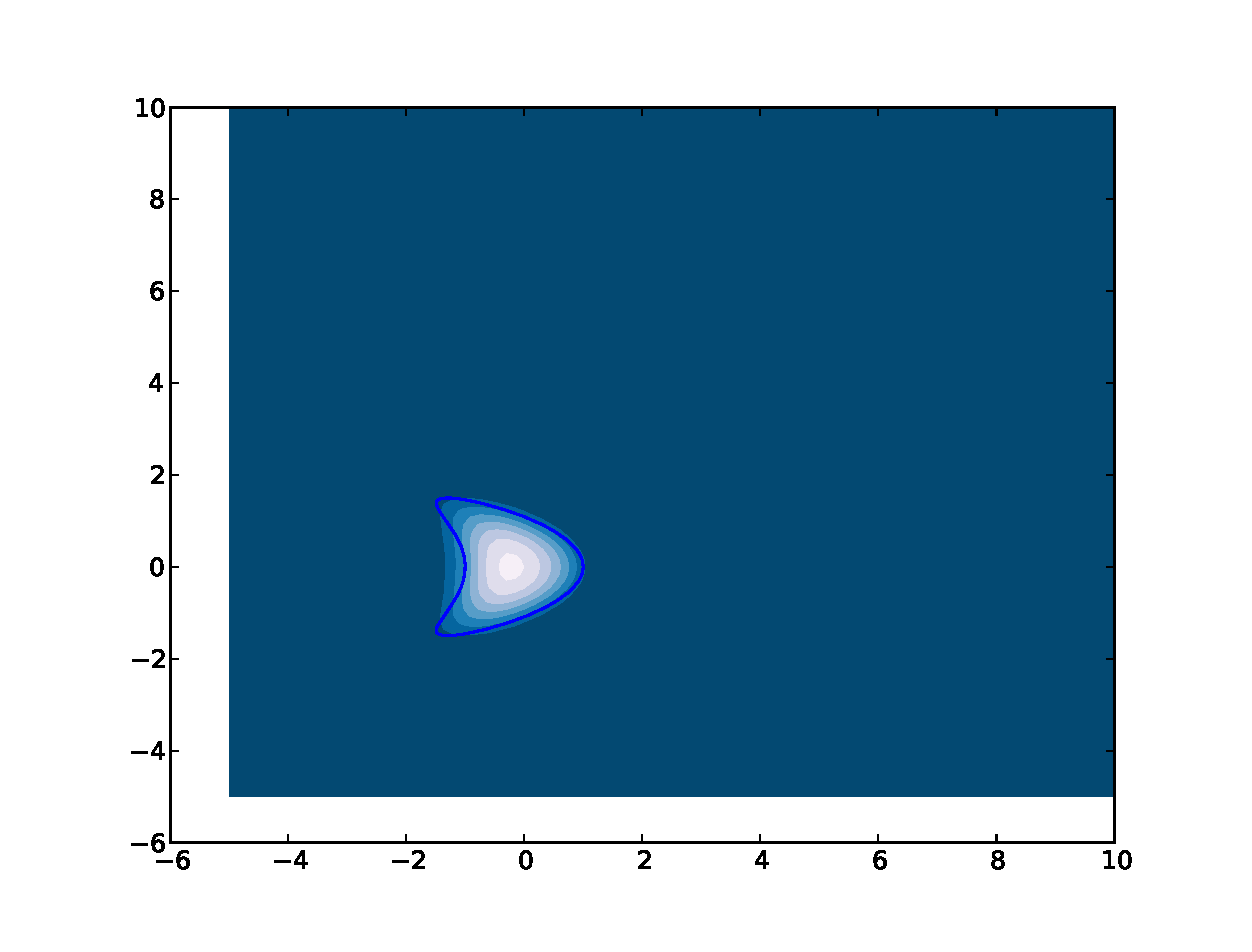
\includegraphics[scale=0.6]{src/data/achiral_chiral_TM.eps}
  \caption{Achiral-Chiral Reconstruction}  
\label{fig:a-c-tm}
\end{figure}

\appendix

\chapter{Symbolic Manipulation Procedures}

In order to automate the equation derivation processes and to eliminate the inaccuracies in the numerical codes and the final \TeX\,output, a few programs have been written. 

The main program is written in the open-source computer algebra system \href{http://maxima.sourceforge.net/}{\textbf{maxima}}. 

%\lstinputlisting[lastline=113,caption=The main symbolic program. For brevity the 2d chiral-chiral case is shown.]{src_new/ansatz_2d.mac}\label{lst:mac}
%\lstinputlisting[caption=Numerical python and \TeX\,code generator.]{src_new/code_generator.py}
%\lstinputlisting[caption=Domain and kernel definitions used in computation.]{src_new/op.py}
%\lstinputlisting[caption=Generated numerical python program for chiral-chiral case.]{src_new/em_chiral_chiral_test.py}

\nocite{*}
\bibliographystyle{plainnat}
\bibliography{thesis}
\end{document}

%A simple lemma. The operators can be written as a linear combinations of operator differences if and only if the coefficients sum to zero.
